\documentclass[10pt]{article}
\usepackage{mathtools}
\usepackage{amsthm}
\usepackage{amssymb}
\usepackage{tikz,lipsum,lmodern}
\usepackage[most]{tcolorbox}
\usepackage{cancel}
\usepackage{hyperref}
\hypersetup{
    colorlinks,
    citecolor=black,
    filecolor=black,
    linkcolor=black,
    urlcolor=black
}
\newcommand{\bottom}[1]{\begin{tcolorbox}[enhanced,colback=white,colframe=black]
    #1
\end{tcolorbox}}

\newcommand{\bottomp}[1]{\begin{tcolorbox}[enhanced,colback=white,colframe=black]
    \begin{proof}
        #1
    \end{proof}
\end{tcolorbox}}

\title{Algebra}
\author{Manuel Mignogna}

\begin{document}

\maketitle
\tableofcontents
\section{Assiomi}
\subsection{Assioma del Vuoto}
\bottom{
    Esiste un insieme, detto l'insieme vuoto $\emptyset$,
    che non contiene nulla.
    $$\exists\emptyset\ (\forall x\ (x\not\in\emptyset))$$
}

\subsection{Assioma di Estensionalità}
\bottom{
    Due insiemi coincidono se e solo se
    ogni elemento del primo insieme appartiene al secondo e viceversa.
    $$\forall x,y\ ( x=y \iff \forall z\ (z\in x \iff z\in y))$$
}

\subsection{Assioma di Separazione}
\bottom{
    Esiste sempre l'insieme degli elementi di un insieme $s$ che verificano un predicato $\rho$.
    $$\{x\ |\ x\in s \land \rho(x)\}$$
}

\subsection{Assioma di Esistenza dell'insieme delle Parti}
\bottom{
    Per ogni insieme $s$ esiste l'insieme delle parti $\mathcal P(s)$, ovvero l'insieme di tutti i sottoinsiemi di $s$.
    $$\forall s \ \exists\mathcal P(s)\ (\forall x\ (x\in \mathcal P(s) \iff x\subseteq s))$$
}

\subsection{Assioma della Coppia}
\bottom{
    Per ogni coppia si insiemi $x,y$ esiste l'insieme coppia $\{x,y\}$.
    $$\forall x,y\ \exists c\ (\forall z\ (z\in c \iff (z=x \lor z=y)))$$
}

\subsection{Assioma di Unione}
\bottom{
    Per ogni insieme di insiemi $a$ esiste l’insieme
    unione unaria di $a$, cioè l’insieme unione di tutti gli insiemi che sono elementi
    di $a$.
    $$\forall a\ \exists u\ (\forall x\ (\exists y\ (x\in u \iff (x\in y \land y \in a))))$$
}

\subsection{Assioma della Scelta}
\bottom{
   Data una famiglia non vuota di insiemi non
    vuoti esiste una funzione che ad ogni insieme della famiglia fa corrispondere un
    suo elemento.
}

\subsection{Assioma dell'infinito}
\bottom{
    Esiste un insieme infinito, e tale insieme è $\mathbb N$.
}

\section{Teoremi derivanti dagli assiomi}
\subsection{Unicità dell'insieme vuoto}
\bottomp{
    Siano $a$ e $b$ due insiemi vuoti. Dalla definizione di insieme vuoto segue che, per ogni elemento generico $x$:
    $$\forall x\ (x\not\in a \land x\not\in b)$$
    Le implicazioni
    $$x\in a \implies x\in b$$
    $$x\in b \implies x\in a$$
    sono entrambe vere perchè l'antecedente è sempre falso.\\
    Pertanto per l'assioma di estensionalità
    $$(x\in a \iff x\in b) \implies a=b$$
    Quindi esiste un unico insieme vuoto.
}

\subsection{Ogni insieme contiene l'insieme vuoto}
\bottomp{
    La formula
    $$\forall z\ (z\in \emptyset \implies z\in \emptyset)$$ 
    è una tautologia perchè $z\in \emptyset$ è sempre falso e dunque l'implicazione è vera. Pertanto $\emptyset \subseteq \emptyset$.
    Similarmente, la formula
    $$\forall x\ \forall z\ (z\in\emptyset \implies z\in x)$$
    è una tautologia, pertanto $\forall x\ (\emptyset\subseteq x)$
}

\subsection{Unicità dell'insieme delle parti}
\bottomp{
    Sia $x$ un insieme e siano $u$ e $w$ insiemi delle sue parti. Dall’assioma
    di esistenza dell’insieme delle parti abbiamo che 
    $$\forall z\ (z\in u \iff z\subseteq x)$$
    $$\forall z\ (z\in w \iff z\subseteq x)$$
    Da questo segue che 
    $$\forall z\ (z \in u \iff z \subseteq x \iff z \in w)$$
    e quindi
    $$\forall z\ (z \in u  \iff z \in w)$$
    Dall’assioma di estensionalità si ha dunque
    che $u = w$.
}

\subsection{Paradosso di Russel}
\bottom{
    Non esiste l’insieme degli insiemi che
    non appartengono a se stessi.
}
\bottomp{
    Ipotizziamo per assurdo che tale insieme esita
    $$r :=\{ x\ |\ x\not\in x\}$$
    Esistono solo due possibilità: $r\in r$ oppure $r\not\in r$.
    Se $r\in r$, allora per definizione non appartiene a sé stesso
    $$r\in r \implies r\not\in r$$
    il che è chiaramente assurdo.
    Se $r\not\in r$, allora è un insieme che non appartiene a se stesso, e deve per definizione appartenere a se stesso
    $$r\not\in r \implies r \in r$$
    il che è chiaramente assurdo.
}

\subsection{L'insieme di tutti gli insiemi non esiste}
\bottomp{
    Sia \(f(x) = \neg (x \in x)\) ed assumiamo per assurdo che esista $I$ l'insieme di tutti gli insiemi. Allora, definiamo \(r = \{x \in I \mid f(x)\}\), che dovrebbe esistere per l'assioma di separazione ma che non può esistere per il paradosso di Russell. Si ha quindi l'assurdo.
}

\subsection{Parti del Vuoto}
\bottom{$\emptyset$ è un insieme, quindi dall’assioma di esistenza dell’insieme delle parti segue che deve esistere $P(\emptyset)$. A cosa è uguale?
$$\mathcal P(\emptyset)=\{x\subseteq\emptyset \iff \forall z\ (z\in x \implies z\in \emptyset) \}$$
C’è un solo insieme tale che ogni suo elemento z appartiene anche all’insieme
vuoto... l’insieme vuoto stesso!

Pertanto $\mathcal P(\emptyset)=\{\emptyset\}$ cioé il singleton dell'insieme vuoto. Proviamo adesso a chiederci, chi è $\mathcal P(\mathcal P(\emptyset))$, cioè $\mathcal P(\{\emptyset\})$.

Un insieme è sottoinsieme di $\{\emptyset\}$ soltanto se è l’insieme vuoto (abbiamo dimostrato tramite un teorema che l'insieme vuoto è sottoinsieme di ogni insieme) oppure se è $\{\emptyset\}$ stesso (dato che
ogni insieme è proprio sottoinsieme). Da questo segue che:
$$\mathcal P(\mathcal P(\emptyset)) = \mathcal P(\{\emptyset\})= \{\emptyset,\{\emptyset\}\}$$}
\section{Operazioni tra Insiemi}
\subsection{Leggi di De Morgan}
\bottom{
    $\forall a, b, c$
    $$c - (a \cup b) = (c - a) \cap (c - b)$$
    $$c - (a \cap b) = (c - a) \cup (c - b)$$
}
\bottomp{
    \begin{align*}
        c - (a \cup b) &= \{z \in c \mid \neg(z \in (a \cup b))\} \text{ (def. di diff. di insiemi)} \\
        &= \{z \in c \mid \neg (z \in a \lor z \in b)\} \text{ (def. di unione)} \\
        &= \{z \in c \mid \neg(z \in a) \land \neg(z \in b)\} \text{ (De Morgan)} \\
        &= \{z \mid (z \in c) \land (\neg(z \in a) \land \neg(z \in b))\} \text{ (ass. di separazione)} \\
        &= \{z \mid ((z \in c) \land \neg(z \in a)) \land ((z \in c) \land \neg(z \in b))\}\\ &\text{ (distrib. di and su and)} \\
        &= \{z \mid (z \in (c - a)) \land (z \in (c - b)\} \text{ (def. di diff. di insiemi)} \\
        &= (c - a) \cap (c - b) \text{ (def. di intersezione)}
        \end{align*}
}

\subsection{Unione di Insiemi}
\bottom{
    Dati due insiemi $A$ e $B$, definiamo:

    $$A \cup B = \bigcup\{A, B\}$$
    
    Questo insieme esistente sicuramente grazie agli assiomi d'unione e della coppia.
}

\subsection{Intersezione di Insiemi}
\bottom{
    Dati due insiemi $A$ e $B$, definiamo:

    $$A \cap B = \{x \mid x \in A \land x \in B\}$$

    Che è un insieme sicuramente esistente per l'assioma di separazione.
}

\subsection{Insiemi Disgiunti}
\bottom{
    Due insiemi \(a\) e \(b\) si dicono disgiunti se e solo se \(a \cap b = \emptyset\)
}

\subsection{Differenza di Insiemi}
\bottom{
    Dati due insiemi $A$ e $B$, definiamo la differenza di insiemi come:

    $$B - A = \{ Z \in B \mid Z \notin A\}$$

    Che è sicuramente un insieme grazie all'assioma di separazione.
}

\subsection{Differenza Simmetrica di Insiemi}
\bottom{
    Definiamo la differenza simmetrica di $a$ e $b$ come:

    $$a \triangle b = \{x \in a \cup b \mid x \in a \oplus x \in b\}$$
    
    Che è un insieme sicuramente esistente per l'assioma di separazione.
}

\subsection{Coppia Ordinata}
\bottom{
    Dati $x$, $y$ due insiemi. Allora definiamo la coppia ordinata $(x, y)$ come:

    $$(x, y) := \{\{x\}, \{x, y\}\}$$
}

\subsection{Caratterizzazione di Coppie Ordinate}
\bottom{
    $$x = y \iff (x, y) = (y, x)$$
}
\bottomp{
    Dimostriamo $$x = y \implies (x, y) = (y, x)$$ Si ha che:

    $$x = y \implies (\{x\} = \{y\}) \land (\{x, y\} = \{y, x\} = \{x, x\} = \{x\})$$
    E dunque:

    $$(x, y) = \{\{x\}, \{x, y\}\} = \{\{x\}, \{x\}\} = \{\{x\}\}$$ 
    $$(y, x) = \{\{y\}, \{y, x\}\} = \{\{x\}, \{x\}\} = \{\{x\}\}$$
    Dunque $(x, y) = (y, x)$\\
    Dimostriamo $$(x, y) = (y, x) \implies x = y$$

    Allora $$\{\{x\}, \{x, y\}\} = \{\{y\}, \{y, x\}\}$$ e dunque \(\{x\}\) è membro sia del primo insieme che del secondo per estensionalità e allora $$\{x\} = \{y\} \lor \{x\} = \{x, y\}$$ In entrambi i casi, ciò implica la tesi.
}

\subsection{Ennupla Ordinata}
\bottom{
    Iniziamo col definire la terna ordinata come:

    $$(x, y, z) = ((x, y), z)$$

    Dunque, dati n+1 elementi \(i_1, i_2, i_3, ..., i_n, i_{n+1}\) allora definiamo la ennupla ordinata di n+1 elementi come:

    $$(i_1, i_2, i_3, ..., i_n, i_{n+1}) = ((i_1, i_2, i_3, ..., i_n), i_{n+1})$$
}
\subsection{Prodotto Cartesiano}
\bottom{
    $$a\times b := \{z\in \mathcal P(\mathcal P(a \cup b))\ |\ \exists x,y\ (x\in a \land y\in b \land z=(x,y))\}$$
}
\subsection{Corrispondenza fra Insiemi}
\bottom{
    Dati due insiemi $a$ e $b$ e \(g \subseteq a \times b\), la coppia ordinata \((a \times b, g)\) si definisce corrispondenza fra $a$ e $b$ di grafico $g$.
}
\bottom{
    Data una corrispondenza fra due insiemi $a$ e $b$ \(\rho = (a \times b, g)\). Dati \(x \in a\) e \(y \in b\) scriveremo:

    $$x \rho y \iff (x, y) \in g$$

    e diremo che $x$ ed $y$ sono in corrispondenza o relazione fra loro.
}
\bottom{
    \(\rho = (a \times b, g)\)
    $$\forall x \in a$$
    $$\forall y \in b$$
    $$(x, y) \in g \iff \varphi(x, y)$$

    Cioè stiamo definendo g in base ad una proprietà definita dalla formula binaria \(\varphi(x_1, x_2)\).
}


\subsection{Definizione di Relazione Binaria}
\bottom{
    Dato un insieme $a$, una corrispondenza fra $a$ ed $a$ stesso si definisce relazione binaria.
}

\subsection{Insieme delle Corrispondenze}
\bottom{
    Dati due insiemi $a$ e $b$, notiamo con \(CORR(a, b)\) l'insieme delle corrispondenze definibili fra $a$ e $b$.
}

\subsection{Insieme delle Relazioni}
\bottom{
    Dato un insieme $a$, notiamo con \(REL(a)\) l'insieme delle relazioni binarie definibili su $a$. Si nota chiaramente che \(REL(a) = CORR(a, a)\).
}

\subsection{Definizione di Applicazione/Funzione}
\bottom{
    Sia $f$ una corrispondenza fra due insiemi $a$ e $b$. La definiremo:

    $$f = (a \times b, g) \text{ applicazione} :\iff \forall x \in a\ \exists! y \in b\ (x f y)$$

    Che equivale a dire:

    $$f = (a \times b, g) \text{ applicazione} :\iff \forall x \in a\ \exists! y \in b\ ((x, y) \in g)$$
    Descrizione esplicita di una funzione
    $$f: x \in a \mapsto f(x) \in b$$

    Esempio: \(f: x \in \mathbb{N} \mapsto (n+1) \in \mathbb{N}\)
}

\subsection{Dominio e Codominio di un'Applicazione}
\bottom{
    Data un'applicazione \(f = (a \times b, g)\), chiameremo $a$ il dominio di $f$ e $b$ il codominio di $f$.
}

\subsection{Immagine di un'Applicazione}
\bottom{
    Data una funzione \(f = (a \times b, g)\), definiremo l'insieme immagine di $f$ 
    $$Im(f) = \{ y \in b \mid \exists x \in a\ (f(x) = y)\}$$
}
\bottom{
    Definizione Alternativa Semplificata della Notazione di $Im(f)$
$$Im(f) = \{ f(x) \mid x \in a\}$$

Chiaramente questa non è, da sola una formula ben formata, ed è per questo che utilizziamo la definizione originale di $Im(f)$.

}

\subsection{Funzione Ben Posta}
\bottom{
    Definiremo come ben posta ogni corrispondenza che sia un'applicazione. Ovviamente, ciò è equivalente a dire che la funzione è, difatti, una funzione. E' un modo colloquiale per assicurare che una data corrispondenza che chiamiamo funzione è una funzione per davvero, dato che non è sempre ovvio se una corrispondenza sia una funzione o meno.
}

\subsection{Definizione di Prodotto Relazionale (o tra Corrispondenze)}
\bottom{
    Siano $a$, $b$, $c$, $d$ insiemi  e siano \(\rho = (a \times b, g_1)\) e \(\sigma = (c \times d, g_2)\) due corrispondenze.
    Definiamo quindi il prodotto relazionale come la corrispondenza \(\rho\sigma = (a \times d, g_3)\) tale che:

    $$\forall x \in a$$
    $$\forall y \in d$$
    $$(x, y) \in g_3 \iff \exists z\ ((x, z) \in g_1 \land (z, y) \in g_2)$$
}

\subsection{Associatività del Prodotto Relazionale}
\bottom{
    Date tre corrispondenze $\sigma,\rho,\varphi$, volgiamo dimostrare che:
    $$\sigma(\rho\varphi)=(\sigma\rho)\varphi$$
}
\bottomp{
    $$(x,y)\in g_{\sigma(\rho\varphi)} \implies \exists z:\ (x,z)\in g_\sigma \land (z,y)\in g_{\rho\varphi}$$
    $$\implies \exists w:\ (z,w)\in g_\rho \land (w,y)\in g_{\varphi}$$
    $$\implies (x,w)\in g_{\sigma\rho} \land (w,y)\in g_{\varphi}$$
    $$\implies (x,y)\in g_{(\sigma\rho)\varphi}$$
    La dimostrazione inversa è analoga.
}

\subsection{Composizione di Applicazioni}
\bottom{
    Date due funzioni $$f: a \to b$$ $$g: b \to c$$ definiamo la funzione $$g \circ f = fg$$ (cioè prodotto relazionale di $f$ e $g$), e la chiamiamo "$g$ composta $f$" o "composta di $g$ e $f$".\\
    Forma esplicita della composizione di funzioni
    $$g \circ f: x \in a \to g(f(x)) \in c$$
}

\subsection{Funzione Immersione}
\bottom{
    Siano due insiemi \(a, b: a \subseteq b\). Allora la funzione $$f: x \in a \to x \in b$$ si dice immersione di $a$ in $b$.
}

\subsection{Funzione Identità}
\bottom{
    La funzione $$Id_a : x \in a \to x \in a$$ si dice identità di a.
}

\subsection{Restrizione di una Funzione}
\bottom{
    Data una funzione \(f: a \to b\), definito \(s \subseteq a\), allora definiamo la restrizione di $f$ in $s$ la funzione:

    $$f_{\mid s}: x \in s \mapsto f(x) \in b$$
}

\subsection{Prolungamento di una Funzione}
\bottom{
    Data una funzione \(f: a \to c\), una funzione \(g: b \to c\) si dice prolungamento di f se \(\exists s \subseteq b: g_{\mid s} = f\), cioè se esiste un sottoinsieme di $b$ uguale ad $a$.
}

\subsection{Funzione Ridotta / Riduzione di una Funzione}
\bottom{
    Dati $f: a \to b$, $s \subseteq b: Im_f \subseteq s$, la funzione $$g: x \in a \mapsto f(x) \in s$$  si chiama ridotta di $f$ ad $s$.
}

\subsection{Applicazione Costante}
\bottom{
    Dati due insiemi \(a, b\) e \(\overline{y} \in b\). La funzione $$f: x \in a \to \overline{y} \in b$$ si dice funzione costante di valore \(\overline{y}\)
}

\subsection{Funzione Immagine}
\bottom{
    $$\overrightarrow{f}:\ \overline{a}\in\mathcal P(a) \to  \{ f(z)\ | \ z\in \overline{a}\}\in \mathcal P(b)$$
}
\subsection{Funzione Antimmagine}
\bottom{
    $$\overleftarrow{f}:\ \overline{b}\in\mathcal P(b) \to  \{ z\in a\ | \ f(z)\in \overline{b}\}\in \mathcal P(a)$$
}

\subsection{Immagine di un Insieme}
\bottom{
    Dato un insieme $a$ e una funzione $f: a \to b$, definiamo l'immagine di $a$ come:
    $$Im(a)=\{f(x)\ |\ x\in a\}$$
}

\subsection{Antimmagine di un Insieme}
\bottom{
    Data una funzione \(f: a \to b\) ed un insieme \(s \subseteq b\), definiamo l'antimmagine (o controimmagine, preimmagine, immagine inversa) dell'insieme $s$ per la funzione $f$ come l'insieme:

    $$\overleftarrow{f}(s)=\{z \in a \mid f(z) \in s\}$$

}
\subsection{Immagine del Dominio ed Antimmagine del Codominio}
\bottom{
    Per ogni funzione \(f: a \to b\) si osserva che:

    $$\overrightarrow{f}(a) = Im(f)$$
    $$\overleftarrow{f}(b) = a$$
}
\subsection{Immagine ed Antimmagine dell'Insieme Vuoto}
\bottom{
    Per ogni \(f: a \to b\), si ha:

    $$\overrightarrow{f}(\emptyset) = \overleftarrow{f}(\emptyset) = \emptyset$$
}

\subsection{Funzione Suriettiva}
\bottom{
    Una funzione $f: a \to b$ si dice \textit{suriettiva} se e soltanto se:
    $$Im(f)=b$$
    oppure in modo più esplicito
    $$\forall y\in b\ (\exists x\in a\ (f(x)=y))$$
    Negazione della suriettiva
    $$\exists y \in b\ (\forall x \in a\ (f(x) \neq y))$$
}

\subsection{Funzione Iniettiva}
\bottom{
    Una funzione $f: a \to b$ si dice \textit{iniettiva} se e soltanto se:
    $$\forall x,y\in a\ (f(x)=f(y) \iff x=y)$$
    oppure analogamente
    $$\forall x,y\in a\ (x\not=y \implies f(x)\not=f(y))$$
    Negazione dell'iniettiva
    $$\exists x, y \in a\ (f(x) = f(y) \land x \neq y)$$
}

\subsection{Funzione Biettiva}
\bottom{
    Una funzione $f: a \to b$ si dice \textit{biettiva} se e soltanto se:
    $$\forall y\in b\ (\exists! x\in a\ (f(x)=y))$$
    ovvero se è iniettiva e suriettiva\\
    Negazione della biettività
    $$(\exists y \in b)(\forall x \in a)(f(x) \neq y) \lor (\exists x, y \in a)(f(x) = f(y) \land x \neq y)$$
}

\subsection{Definizione di Iniettivà tramite Antimmagine}
\bottom{
    Una funzione è iniettiva se e soltanto se per ogni singleton sottoinsieme del suo codominio, la sua antimmagine è vuota o ha un solo elemento.
    $$\forall y \in \mathcal P_1(b)$$
    $$ \overleftarrow{f}(y)=\emptyset \lor \exists!x\in a\ (\overleftarrow{f}(y)=\{x\})$$
}
\bottomp{
    DIM \(\Rightarrow\):
    Sia \(y \in \mathcal{P}_1(b)\) e supponiamo che \(\overleftarrow{f}(y) \neq \emptyset\). Allora, dalla definizione di antimmagine \(\exists x(f(x) \in y)\). Ma, essendo f iniettiva, si ha che $$\forall z \in a\ (f(z) = y \iff z = x)$$ e dunque \(\overleftarrow{f}(y) = \{x\}\)

    DIM \(\Leftarrow\):
    Siano \(x, y \in a\) tali che \(f(x) = f(y)\). Allora $$\overleftarrow{f}(\{f(x)\}) = \overleftarrow{f}(\{f(y)\}) = \{x\} = \{y\} \implies x = y$$ e dunque la funzione è iniettiva. 
}

\subsection{Definizione di Suriettività tramite Antimmagine}
\bottom{
    Una funzione è suriettiva se e soltanto se per ogni singleton sottoinsieme del suo codominio,
    la sua antimmagine è non vuota
    $$\forall y \in \mathcal P_1(b)\smallsetminus\{\emptyset\}\ \overleftarrow{f}(y)\not=\emptyset$$
}
\bottomp{
    DIM \(\Rightarrow\):
$$\text{f suriettiva } \implies (\forall y \in b)(\exists x \in a)(f(x) = y) \implies$$
$$\implies (\forall \{y\} \in \mathcal{P}_1(b))(\exists x)(x \in \overleftarrow{f}(\{y\})$$

DIM \(\Leftarrow\):
$$(\forall y \in \mathcal{P}_1(b) - \{\emptyset\})(\overleftarrow{f}(y) \neq \emptyset)\implies$$ $$\implies (\forall y \in b)(\exists x \in \overleftarrow f(y))(f(x)= y) \implies \text{f suriettiva}$$
}

\subsection{Definizione di Biettività tramite Antimmagine}
\bottom{
    Una funzione è biettiva se e soltanto se per ogni singleton sottoinsieme del suo codominio,
    la sua antimmagine è un singleton
    $$\forall y \in \mathcal P_1(b)\ \overleftarrow{f}(y)=\{x\}$$
}

\subsection{Sezione di una funzione}
\bottom{
    Date due funzioni $f: a \to b$ e $g: b\to  a$, se
    $$f\circ g = id_b$$
    $g$ si dice sezione di $f$
}

\subsection{Retazione di una funzione}
\bottom{
    Date due funzioni $f: a \to b$ e $g: b\to  a$, se
    $$g\circ f = id_a$$
    $g$ si dice retrazione di $f$
}
\subsection{Caratterizzazione di Iniettività tramite Retrazione}
\bottom{
    Una funzione è iniettiva se e soltanto se il suo dominio è vuoto o esiste una sua retrazione.
    $$a=\emptyset \lor \exists g:b\to  a\ (g\circ f = id_a)$$
}
\bottomp{
    Dimostrazione \(\Leftarrow\):
    Se $a$ è l'insieme vuoto, si verifica banalmente l'iniettività. Se $$(\exists g: b \to a)(g \circ f = id_a)$$ allora essendo \(id_a\) iniettiva, f è iniettiva.\\
    Questo perchè se $f$ non fosse iniettiva allora esisterebbero $x_1, x_2 \in a$ tali che $x_1 \neq x_2$ e $f(x_1) = f(x_2)$. Ma allora $$(g \circ f)(x_1) = g(f(x_1)) = g(f(x_2)) = (g \circ f)(x_2)$$ e dunque $g \circ f$ non sarebbe iniettiva, il che è assurdo perchè $id_a$ è iniettiva.\\
    Dimostrazione \(\Rightarrow\):
    Definisco la funzione $$g: y \in b \mapsto \begin{cases}
    x_y \text{ se } y \in Imf \\
    \overline{x} \text{ se } y \notin Imf
    \end{cases}$$

    Dove \(x_y\) è definito come l'unico elemento di \(\overleftarrow{f}(\{y\})\) (vedi "Caratterizzazione dell'Iniettività tramite Antimmagine"). Si verifica semplicemente che g è una retrazione:
    $$g \circ f(x) = g(f(x)) = g(y) = x_y$$ tale che $$f(x_y) = f(x) \implies x_y = x$$ per iniettività di f, e quindi la funzione g è una retrazione.
}

\subsection{Caratterizzazione di Suriettività tramite Sezione}
\bottom{
    Una funzione è suriettiva se e soltanto se esiste una sua sezione.
    $$\exists g:b\to  a\ (f\circ g = id_b)$$
}
\bottomp{
    Dimostrazione \(\Leftarrow:\)
    $$(\exists g: b \to a)(f \circ g = id_b)$$ implica che f sia suriettiva dato che \(id_b\) è suriettiva.\\
    Questo perchè se $f$ non fosse suriettiva allora esisterebbe $y \in b$ tale che \(\overleftarrow{f}(\{y\}) = \emptyset\). Ma allora $$(f \circ g)(y) = f(g(y)) = f(x)$$ per qualche \(x \in a\), ma allora \(x \notin \overleftarrow{f}(\{y\})\) e quindi \(f(x) \neq y\), il che è assurdo perchè \(id_b\) è suriettiva.\\
    Dimostrazione \(\Rightarrow\):
    Dalla caratterizzazione di suriettività tramite antimmagine si ha che $$\text{f è suriettiva } \iff \forall y \in b\ (\overleftarrow{f}(\{y\}) \neq \emptyset)$$ Per l'assioma della scelta esiste la funzione $$\varphi: \overleftarrow{f}(\{y\}) \in \mathcal{P}(a) \mapsto (x \in a)(x \in \overleftarrow{f}(\{y\}))$$

    Definiamo quindi $$g: y \in b \mapsto \varphi(\overleftarrow{f}(\{y\})) \in a$$ che è una sezione in quanto:
    $$f \circ g(y) = f(g(y)) = f(\varphi(\overleftarrow{f}(\{y\}))) = y$$
}

\subsection{Inversa di una Funzione}
\bottom{
    Date due funzioni \(f: a \to b\) e \(g: b \to a\), se g è sia retrazione che sezione di f, allora g si dice inversa di f.
}

\subsection{Caratterizzazione della Biettività tramite Inversa}
\bottom{
    Una funzione è biettiva se e soltanto se esiste una sua inversa.
    $$\exists g:b\to  a\ (f\circ g = id_b) \land (g\circ f = id_a)$$
}

\subsection{Unicità dell'Inversa}
\bottom{
    Se una funzione $f$ che ha una sezione $s$
    ed una retrazione $r$, allora si ha che $r = s$ ed essa è la sua unica inversa.
}
\bottomp{
    $$r\circ f=id_a \land f\circ s=id_b$$
    allora
    $$(r\circ f)\circ s=id_a\circ s=s$$
    $$r\circ(f\circ s)= r\circ id_b=r$$
    Ma per l'associatività del prodotto relazionale
    $$(r\circ f)\circ s=r\circ(f\circ s)$$
    e dunque $r=s$.
}

\subsection{Una funzione con una sola sezione è biettiva}
\bottom{Se una funzione
$f$ ha una ed una sola sezione $s$, allora essa è una funzione biettiva ed $s$ è la sua
inversa.}
\bottomp{
    $$(\exists! g: b \to a)(f \circ g = id_b) \implies (\forall y \in b)(\exists! x \in a)(f(x) = y)$$

    Supponiamo per assurdo che \(\exists x_1, x_2 \in a: x_1 \neq x_2 \land f(x_1) = f(x_2) = y\), cioè che f non sia iniettiva. Ciò implica che possono esistere \(g_1, g_2\) sezioni distinte (definite in basso) tali che \(g_1(y) = x_1\) e \(g_2(y) = x_2\), il che va contro l'ipotesi. Quindi $f$ dev'essere iniettiva, il che implica che essa abbia una retrazione. Avendo entrambe una sezione ed una retrazione, esse coincidono e sono anche l'inversa, e dunque la funzione è biettiva.

    $$g_1: g(f(x_1)) = x_1$$
    $$g_2: y \in b \mapsto \begin{cases}
    g(y) \text{ se } y \neq f(x_1) \\
    x_2 \text{ se } y = f(x_2)\end{cases}$$
}

\subsection{Affermazioni equivalenti alla Biettività}
\bottom{
    \begin{enumerate}
        \item $f$ è biettiva
        \item $f$ ha inversa
        \item $f$ ha sezioni e retrazioni
        \item $f$ ha una sola sezione
        \item $\forall y\in b\ (\exists!x\in a\ (f(x)=y))$
    \end{enumerate}
}




\section{Strutture Algebriche}

\subsection{Struttura algebrica}
\bottom{
    Una ennupla ordinata del tipo:
    $$(s,*_1,*_2,\dots,*_n)$$
    dove $s\not=\emptyset$ si dice insieme di sostegno, e $*_k$ sono le operazioni, si dice struttura algebrica.}

\subsection{Operazione Interna}
\bottom{
    Dato un insieme $s\not=\emptyset$, una funzione
    del tipo $$*:s\times s\to s$$ si dice operazione interna (binaria dato che
    ha n-arietà uguale a due).
}
\bottom
{
    Se l’applicazione che stiamo usando è un’operazione, non usiamo la normale notazione di funzione, ma piuttosto poniamo il simbolo dell’operazione fra i due
    operandi. Scriviamo cioè 
    $$x*y \text{ invece di } *(x,y)$$
}

\subsection{Commutatività}
\bottom{
    Un’operazione $*$ si dice commutativa se
    $$\forall x,y\in s$$
    $$(x*y=y*x)$$
}

\subsection{Associatività}
\bottom{
    Un’operazione $*$ si dice associativa se
    $$\forall x,y,z\in s$$
    $$x*(y*z)=(x*y)*z$$
    In tal caso possiamo evitare le parentesi e scrivere
    semplicemente $$x*y*z$$
}
\subsection{Operazione Duale o Opposta}
\bottom{
    Data un'operazione \(*: s \times s \to s\), definiamo la sua operazione duale o opposta come \(\overline{*}: s \times s \to s\) tale che: $$\forall x, y \in s\ (x \overline{*} y \iff y * x)$$
}


\subsection{Semigruppo}
\bottom{
    Una struttura algebrica $(s,*)$ si dice semigruppo se $*$ è un’operazione binaria interna associativa su $s$.
}

\subsection{Elemento Neutro}
\bottom{
    Dato un semigruppo $(s,*)$, un elemento $e\in s$ si dice elemento neutro se
    $$\forall x\in s$$
    $$(e*x=x=x*e)$$
}

\subsection{Unicità dell'elemento neutro}
\bottom{
    Dato un semigruppo $(s,*)$, se esiste un elemento neutro, questo è unico.
}
\bottomp{
    Per definizione di elementi neutri a sinistra e a destra:
$$l=l*d=d$$
}

\subsection{Monoide}
\bottom{
    Una struttura algebrica $(s,*)$ si dice monoide se $*$ è un’operazione binaria interna associativa su $s$ e se $s$ ha un elemento neutro rispetto a $*$.

    È possibile notare l’elemento neutro esplicitamente, in tale modo:
    $$(s,*,u)$$
}
\bottom{
    \textbf{Esempio.} $(\mathbb N, +, 0)$ è un monoide, in quanto la somma è associativa e lo zero è elemento neutro.
}

\subsection{Elemento invertibile}
\bottom{
    Dato un monoide $(s,*,u)$, un elemento $x\in s$ si dice invertibile se
    $$\exists y\in s$$
    $$(x*y=u=y*x)$$
    In tal caso $y$ si dice inverso di $x$.
}
\bottom{
    Un elemento invertibile si dice anche simmetrizzabile.

    Un elemento inverso si dice anche elemento simmetrico o elemento opposto.

    Usiamo la dicitura $\mathcal U(s)$ per indicare l’insieme di tutti gli elementi simmetrizzabili di $s$.
}
\subsection{Unicità dell'inverso}
\bottom{
    Dato un monoide $(s,*,u)$, se un elemento $x\in s$ è invertibile, il suo inverso è unico.
}
\bottomp{
    Siano $l$ e $d$ due inversi di $x$:
$$l=l*u=l*(x*d)=(l*x)*d=u*d=d$$
}

\subsection{Gruppo}
\bottom{
    Una struttura algebrica $(s,*)$ si dice gruppo se $*$ è un’operazione binaria interna associativa su $s$, se $s$ ha elemento neutro rispetto a $*$ e se ogni elemento di $s$ è invertibile rispetto a $*$.
}
\bottom{
    Un gruppo $(s,*)$ si dice abeliano se $*$ è commutativa.
}
\bottom{
    \textbf{Esempio.} $(\mathbb Z, +, 0)$ è un gruppo, in quanto la somma è associativa, lo zero è elemento neutro ed ogni intero è invertibile rispetto alla somma.
}


\subsection{Parte Stabile}
\bottom{
    Sia $(s, *)$ una struttura algebrica e sia $t\subseteq s$
    non vuoto. Allora $t$ si dice parte stabile o chiusa di $s$ rispetto a $*$ se e soltanto
    se:
    $$\forall x,y\in t$$
    $$ (x*y\in t)$$
    Cioè se, effettuando un’operazione a partire da elementi di $t$, il risultato è
    ancora in $t$.
}
\bottom{
    \textbf{Esempio.} Sia $(\mathbb R, +)$ una struttura algebrica. Allora $\mathbb N$ è una parte stabile di $\mathbb R$ rispetto alla somma.
    Non è parte chiusa rispetto alla differenza, dato che ad esempio sia 5 che 7 appartengono ad $\mathbb N$ ma
    $(5 - 7) = -2 \not\in \mathbb N$
}
\bottom{
    In generale, per ogni monoide $(s, *, u)$, $\{u\}$ è parte stabile in
    quanto $u*u=u$. Inoltre, $s$ è sempre parte stabile di se stesso.
}

\subsection{Operazine Indotta}
\bottom{
    Sia $(s, *)$ una struttura algebrica e
    $t \subseteq s$ parte stabile, allora si nota che:
    $$*_{|t\times t}=((t\times t)\times t,g)$$
    $$g=\{(x,y,z)\in t\times t\times t\ |\ x*y=z\}$$
    Cioè la ridotta è un’operazione binaria interna del tipo
    $$*_{|t\times t}:t\times t \to t$$

    Definiamo quindi $*_{|t\times t}$ operazione indotta da $*$ su $t$.
}
\bottom{
    Un’operazione indotta conserva sempre le proprietà di commutatività, associatività dell’operazione originale, ma può ”perdere” l’elemento neutro o gli
    inversi se questi non fanno parte della parte chiusa.
}

\subsection{L’intersezione di Parti Stabili è una Parte Stabile}
\bottom{
    Sia $(s, *)$ una struttura algebrica e sia $t \subseteq \mathcal P(s)$ tale che $$\forall x\in t\ (t\text{ parte stabile di }s)$$
    Allora $$\bigcap t\text{ è parte stabile di }s$$
}
\bottomp{
    Siano $x,y\in \bigcap t$. Allora, per la definizione di intersezione unaria
    $$\forall z\in t\ (x,y\in z)$$
    (questo perché $x$ e $y$ appartengono a tutti gli insiemi di $t$)\\

    Essendo ogni $z$ parte stabile di $s$, ciò implica che
    $$\forall z\in t\ (x*y\in z)\iff x*y\in \bigcap t$$
    E dunque $\bigcap t$ è parte stabile di $s$.
}

\subsection{Sottostruttura}
\bottom{
    Sia $(s, *)$ una struttura algebrica e sia $t\subseteq s$ parte stabile. Allora $(t, *_{|t\times t})$ è una struttura algebrica, detta sottostruttura di $(s, *)$.
}
\bottom{
    Se la struttura $(s, *)$ e la sottostruttura $(t, *_{|t\times t})$ hanno le stesse proprietà allora scriveremo $t \leq s$.
}

\subsection{Elemento Neutro di un Sottogruppo}
\bottom{
    Sia $(s, *)$ un gruppo e sia $t\le s$. Allora l’elemento neutro di $t$ è lo stesso di $s$.
}
\bottomp{
   $$1_t\in t\implies 1_t\in s\implies 1_t\cdot 1_t = 1_t = 1_t \cdot 1_s$$
    Il che implica che sia $1_s$ e $1_t$ siano inversi di $1_t$, ma essendo l'inverso unico si ha che $$1_t = 1_s$$
}

\subsection{Sottostruttura Generata}
\bottom{
    Sia $(s, *)$ una struttura algebrica e sia $t\subseteq s$ parte stabile. Allora
    $$\langle t\rangle=\bigcap\{u\le s\ |\ t\subseteq u\}$$
    si dice sottostruttura generata da $t$.
}
\bottom{
    La ragione per cui la chiamiamo ”generata” è che si può dimostrare che
    essa è in realtà l’insieme delle combinazioni lineari dell’insieme $t$.

    Per esempio,
    il sottomonoide generata da 2 di $(\mathbb N, +)$ è l’insieme di tutti i valori che si
    possono ottenere sommando 2
    $$\langle 2\rangle= \{2, 4, 6, 8, 10, 12, 14, 16, 18, 20, \dots \}$$
}

\subsection{Caratterizzazione dei Sottomonoidi Generati}
\bottom{
    Sia $(s, *)$ un monoide e sia $\emptyset\ne t\subseteq s$ parte stabile. Allora:
    $$\langle t\rangle=\{ x\ \in s \mid (\exists n \in \mathbb{N})(\exists x_1, x_2, ..., x_n \in t)(x = x_1 * x_2 * ... * x_n)\} \cup \{ 1_s \}$$
}
\bottomp{
    Caso \(\subseteq\)) chiamiamo l'insieme a destra dell'ipotesi \(b\) per brevità. Consideriamo che:
\begin{itemize}
    \item \(t \subseteq b\), perché se \(x \in t\) scelgo \(n = 1, x_1 = x\implies x \in b\)
    \item  Ogni elemento di \(b\) è esprimibile come composizione di elementi di \(t\) e dunque di \(s\), ed essendo \(*\) un'operazione interna allora \(b \subseteq s\).
    \item L'elemento neutro appartiene a \(b\) per costruzione.
    \item Siano $x, y\in b$, allora per definizione di $b$
    $$(\exists n, m \in \mathbb{N})(\exists x_1, ..., x_n, y_1, ..., y_m)(x = x_1*...*x_n \land y = y_1 * ...* y_n)$$
Questo implica che \(x*y = x_1 * ... * x_n * y_1 * ... * y_n \implies x * y \in b\) e dunque l'operazione indotta è interna.
\end{itemize}
Essendo \(b \leq s \land t \subseteq b\)allora \(<t> \subseteq b\) per la definizione di sottoinsieme generato come l'intersezione di tutte le sottostrutture di tale tipo.

Caso \(\supseteq\)) Vogliamo dimostrare che $$(\forall x \leq s)(t \subseteq x \implies b \subseteq x)$$ poiché da questo segue che \(b \subseteq <t>\), che è la tesi.
Allora, siano \(x \leq s \land t \subseteq x\). Essendo \(x\) parte chiusa, allora $$(\forall n \in \mathbb{N})(\forall y_1, ... y_n \in t \subseteq x)(y_1 * ... * y_n \in x) \implies (\forall y \in b)(y \in x) \implies b \subseteq x$$
Quindi \(b\) è parte di ogni sottostruttura contente \(t\), e dunque parte della loro intersezione, e quindi \(b \subseteq <t>\).
}

\subsection{Caratterizzazione dei Gruppi Generati}
\bottom{
    Sia \((g, *, 1_s)\) un gruppo e sia \(\emptyset \neq t \subseteq g\) parte stabile. Allora:

$$<t> = \{x \in g \mid (\exists n \in \mathbb{N})(\exists \varepsilon_1, \varepsilon_2, ..., \varepsilon_n \in \{-1, 1\})$$
$$(\exists x_1, x_2, ..., x_n \in t)(x = x_1^{\varepsilon_2} * x_2^{\varepsilon_2} * ... * x_n^{\varepsilon_n})\}$$
}
\bottomp{
    Caso \(\subseteq\)) chiamiamo l'insieme a destra dell'ipotesi \(b\) per brevità. Consideriamo che:
\begin{itemize}
    \item \(t \subseteq b\), perché se \(x \in t\) scelgo \(n = 1, \varepsilon_1 = 1, x_1 = x\implies x \in b\)
    \item Ogni elemento di \(b\) è esprimibile come composizione di elementi di \(t \subseteq s\) o dei loro inversi in \(s\), ed essendo \(*\) un'operazione interna allora \(b \subseteq s\).
    \item Se scegliamo $n = 2, \varepsilon_1 = 1, \varepsilon_2 = -1, x_1 = x_2 = x \in t \implies $
    $$(\exists y \in b)(y = x_1^{\varepsilon_1} * x_2^{\varepsilon_2} = x * x^{-1} = 1_s)$$
    \item  Dalle due precedenti segue che ogni elemento di \(b\) è dotato di inverso.
    \item Siano \(x, y \in b\), allora per definizione sono entrambi esprimibili come composizione di \(n, m \in \mathbb{N}\) elementi di \(t\) o loro inversi. Dunque la loro composizione è esprimibile come \(n + m\) elementi di \(t\) o loro inversi, quindi essa appartiene a \(b\) e l'operazione indotta è binaria interna.
\end{itemize}

Essendo \(b \leq s \land t \subseteq b\) allora \(<t> \subseteq b\) per la definizione di sottoinsieme generato come l'intersezione di tutte le sottostrutture di tale tipo.

Caso \(\supseteq\)) Vogliamo dimostrare che $$(\forall x \leq s)(t \subseteq x \implies b \subseteq x)$$ poiché da questo segue che \(b \subseteq <t>\), che è la tesi.
Allora, siano \(x \leq s \land t \subseteq x\). Essendo \(x\) parte chiusa dotata di inversi per ogni elemento, allora $$(\forall n \in \mathbb{N})(\forall \varepsilon_1, ... \varepsilon_n \in \{1, -1\})(\forall y_1, ... y_n \in t \subseteq x)(y_1^{\varepsilon_1} * ... * y_n^{\varepsilon_n} \in x) \implies$$
$$\implies (\forall y \in b)(y \in x) \implies b \subseteq x$$
Quindi \(b\) è parte di ogni sottostruttura contente \(t\), e dunque parte della loro intersezione, e quindi \(b \subseteq <t>\).
}

\subsection{Struttura Ciclica}
\bottom{
    $(s,*)$ è una struttura ciclica $\iff \exists x\in s$ tale che $<x>=s$
}

\subsection{Elemento Cancellabile}
\bottom{
    Sia $(s, *)$ una struttura algebrica e sia $k\in s$. Allora $k$ si dice cancellabile se
    $$\forall x,y\in s$$
    $$k*x=k*y\implies x=y$$
    $$x*k=y*k\implies x=y$$
}
\bottom{Un elemento non è cancellabile quando
$$k\text{ non cancellabile a sx}\iff \exists x,y\in g\ (kx=ky \land x\not=y)$$
$$k\text{ non cancellabile a dx}\iff \exists x,y\in g\ (xk=yk \land x\not=y)$$}

\subsection{Invertibilità implica Cancellabilità}
\bottom{
    Dato un gruppo $(g,\cdot)$
    $$\forall x\ (x\in\mathcal U(g)\implies x\text{ cancellabile})$$
}
\bottomp{$$x\in\mathcal U(g)\implies \exists\Bar{x}\in g\ (x\cdot\Bar{x}=1_g=\Bar{x}\cdot x)$$
    Siano allora $y,z\in g$ tali che 
    $$xy=xz \implies \Bar{x} \cdot x \cdot y = \Bar{x} \cdot x \cdot z \implies 1_g \cdot y = 1_g \cdot z \implies y=z$$
    Analogamente
    $$yx=zx \implies y \cdot x \cdot \Bar{x} = z \cdot x \cdot \Bar{x} \implies y \cdot 1_g = z \cdot 1_g \implies y=z$$
}
\bottom{
    \textbf{Attenzione.} L’opposto non è necessariamente vero: cancellabilità non implica invertibilità. Per esempio, in $(\mathbb Z, \cdot)$ nessun elemento a parte 1 è invertibile, ma tutti sono cancellabili.
}

\subsection{Funzione Traslazione}
\bottom{
    Sia $(s,\cdot)$ un semigruppo e sia $x\in s$.
    $$\sigma_x: z \in s \mapsto x \cdot z \in s \text{ funzione traslazione a sinistra}$$
    $$\delta_x: z \in s \mapsto z \cdot x \in s \text{ funzione traslazione a destra}$$
}
\bottom{
    $x$ è cancellabile a sinistra $\iff$ la funzione traslazione a sx è iniettiva.
    
    $x$ è cancellabile a destra $\iff$ la funzione traslazione a dx è iniettiva.
}

\subsection{Tavola di Cayley}
\bottom
{$$\text{neutro a sx}\iff\text{riga = riga elementi}$$
$$\text{neutro a dx}\iff\text{colonna = colonna elementi}$$
$$\text{invertibile a sx}\iff\text{riga contiene elemento neutro}$$
$$\text{invertibile a dx}\iff\text{colonna contiene elemento neutro}$$
$$\text{operazione commutativa}\iff\text{tavola simmetrica}$$
$$\text{cancellabile a sx}\iff\text{riga con elementi tutti diversi}$$
$$\text{cancellabile a dx}\iff\text{colonna con elementi tutti diversi}$$}

\subsection{Omomorfismi fra Strutture Algebriche}
\bottom{
    Siano $(s, *_s)$ e $(t, *_t)$ due strutture algebriche. Una funzione $f: s \to t$ si dice omomorfismo se
    $$\forall x,y\in s$$
    $$f(x *_s y) = f(x) *_t f(y)$$
}
\bottom{Un’omomorfismo è dunque una funzione che ci permette di ”passare” da una
struttura ad un’altra conservando però le proprietà delle operazioni.
\textbf{Esempio.}
$$EXP: x \in \mathbb{R} \mapsto e^x \in \mathbb{R} - \{0\}$$
Questa funzione è un'omomorfismo fra le strutture $(\mathbb{R}, +)$ e $(\mathbb{R} - \{0\}, \cdot)$ in quanto
$$(\forall x, y \in \mathbb{R})(EXP(x + y) = e^{x + y} = e^x \cdot e^y = EXP(x) \cdot EXP(y))$$}

\subsection{Monomorfismo}
\bottom{
    Un omomorfismo iniettivo si dice monomorfismo.
}

\subsection{Epimorfismo}
\bottom{
    Un omomorfismo suriettivo si dice epimorfismo.
}
\bottom{
    Epimorfismi conservano l’associatività, la commutatività, i neutri, e gli inversi.
}

\subsection{Epimorfismi conservano i Neutri}
\bottomp{
    Siano $(s,*)$ e $(\Bar{s},\Bar{*})$ strutture algebriche,
$\varphi: s \to\Bar{s}$
un'epimorfismo, $1_s\in s$ elemento neutro, e sia $y\in\Bar{s}$.

Essendo la funzione suriettiva
$$\exists x\in s\ (\varphi(x)=y)$$
Allora
$$y\ \Bar{*}\ \varphi(1_s) = \varphi(x)\ \Bar{*}\ \varphi(1_s) = \varphi(x * 1_s) = \varphi(x) = y$$
quindi $\varphi(1_s)$ è elemento neutro di $(\Bar{s},\Bar{*})$
}

\subsection{Epimorfismi conservano la Commutatività}
\bottom{
    Siano \((s, *)\) e \((\Bar{s}, \Bar{*})\) strutt. algebriche tale che \(*\) è un'operazione commutativa e sia \(\varphi: s \to \Bar{s}\) un'epimorfismo. Vogliamo dimostrare che anche l'operazione \(\Bar{*}\) è commutativa.
}
\bottomp{
Siano \(y_1, y_2 \in \Bar{s}\). Essendo la funzione suriettiva $$\exists x_1, x_2 \in s\ (\varphi(x_1) = y_1 \land \varphi(x_2) = y_2)$$ Allora:
$$y_1 \Bar{*} y_2 = \varphi(x_1) \Bar{*} \varphi(x_2) =$$
$$= \varphi(x_1 * x_2) = \varphi(x_2 * x_1) = \varphi(x_2) \Bar{*} \varphi(x_1) = y_2 \Bar{*} y_1$$

E dunque l'operazione \(\Bar{*}\) è commutativa.
}

\subsection{Isomorfismo}
\bottom{
    Un omomorfismo biettivo si dice isomorfismo.
}

\subsection{L'inversa di un isomorfismo è a sua volta un isomorfismo}
\bottom{Siano \((s, *)\) e \((\Bar{s}, \Bar{*})\) due strutture algebriche. Se \(\varphi: s \to \Bar{s}\) è un isomorfismo, allora \(\varphi^{-1}: \Bar{s} \to s\) è a sua volta un isomorfismo.
Se \(\varphi\) è biettiva, allora esiste \(\varphi^{-1}\) anch'essa biettiva. Pertanto, per dimostrare che essa è un isomorfismo, basta dimostrare che è un omomorfismo.

 $$(\forall x, y \in \Bar{s})(\varphi^{-1}(x \Bar{*} y) = \varphi^{-1}(x) * \varphi^{-1}(y))$$
 }
\bottomp{
    Siano \(x, y \in \Bar{s}\). Essendo $$\varphi \circ \varphi^{-1} = id_{\Bar{s}}$$ allora abbiamo che:

    $$\varphi^{-1}(x \Bar{*} y) = \varphi^{-1}(\varphi(\varphi^{-1}(x))\ \Bar{*}\ \varphi(\varphi^{-1}(y)))=$$
    $$ = \varphi^{-1}(\varphi(\varphi^{-1}(x) * \varphi^{-1}(y))) = \varphi^{-1}(x) * \varphi^{-1}(y)$$
}
\bottomp{
    DIMOSTRAZIONE ALTERNATIVA
    $$\varphi(\varphi^{-1}(x) * \varphi^{-1}(y)) = \varphi(\varphi^{-1}(x)) \Bar{*} \varphi(\varphi^{-1}(y)) = x \Bar{*} y$$
Poiché \(\varphi\) è un isomorfismo. Se applichiamo \(\varphi^{-1}\) ad entrambi gli estremi dell'equazione qui sopra, allora otteniamo:

$$\varphi^{-1}(\varphi(\varphi^{-1}(x) * \varphi^{-1}(y))) = \varphi^{-1}(x \Bar{*} y)$$
 
E semplificando le funzioni inverse:

$$\varphi^{-1}(x) * \varphi^{-1}(y) = \varphi^{-1}(x \Bar{*} y)$$

Che è la tesi.
}

\subsection{Automorfismo}
\bottom{
    Un isomorfismo di una struttura algebrica in se stessa ovvero un isomorfismo \(f: a \to a\) si dice automorfismo.
}

\subsection{Anello}
\bottom{Sia \(a \neq \emptyset\) e siano \(+, \cdot\) due operazioni binarie interne di \(a\). La struttura algebrica \((a, +, \cdot)\) si dice anello se \((a, +)\) è un gruppo abeliano, \((a, \cdot)\) è un semigruppo, e vale la proprietà distributiva di $\cdot$ su $+$:

$$\forall x, y, z \in a$$
$$x \cdot (y + z) = x \cdot y + x \cdot z$$}
\bottom{
    Dato un anello \((a, +, \cdot)\), indichiamo con
    \begin{itemize}
        \item \(0_a\) o \(0^N\) l'elemento neutro rispetto all'operazione \(+\)
        \item \(1_a\) o \(1^N\) l'elemento neutro dell'operazione \(\cdot\) (se esiste)
    \end{itemize}
}
\bottom{Dato un anello \((a, +, \cdot)\), allora definiamo:
\begin{itemize}
    \item \(\forall x, y \in a\ (x - y = x + (-y))\)
    \item \(\forall x \in a\\\forall n \in \mathbb{N} - \{0\}\\ nx = x + x + ... + x \text{ (} n \text{ volte)})\)
    \item \(\forall x \in a\\ \forall n \in \mathbb{Z} - \mathbb{N}\\ nx = -x - x - ... - x \text{ (} n \text{ volte)})\)
    \item \(\forall x \in a\ (0x = 0_a)\)
\end{itemize}
 
Stiamo dunque definendo la differenza, e i multipli.}
\bottom{
    Dato un anello \((a, +, \cdot)\), allora definiamo le proprietà del prodotto:
    \begin{enumerate}
        \item $\forall x \in a\\ \forall n \in \mathbb{N} - \{0\}$
        $$ x^n = x \cdot x \cdot ... \cdot x \text{ (} n \text{ volte)}$$
        \item $\forall x \in a\\ \forall n \in \mathbb{N}- \{0\}$
        $$ x^{-n} = x^{-1} \cdot x^{-1} \cdot ... \cdot x^{-1} \text{ (} n \text{ volte)}$$
        \item $\forall x \in a$
        $$ x^0 = 1_a \text{ (se esiste)}$$
        Con queste prime tre proprietà stiamo dunque definendo la potenza per l'anello.
        \item
        $\forall x,y,z \in a$
        $$ x \cdot (y - z) = x \cdot (y + (-z)) = xy + x(-z) = xy - xz$$
        \item Per la (4), è dunque distributivo rispetto alla differenza:\\ 
        $$\forall x, y \in a\ (x \cdot (-y) = -xy = (-x)y)$$
        \item Se l'anello è unitario:\\
        $\forall x \in a\\
        \forall n \in \mathbb{N}$
        $$(n \cdot 1_a)x = nx$$
    \end{enumerate}
}
\subsection{Anello Commutativo}
\bottom{
    Un anello \((a, +, \cdot)\) si dice commutativo se \((a, \cdot)\) è un semigruppo commutativo.
}

\subsection{Anello Unitario}
\bottom{
    Un anello \((a, +, \cdot)\) si dice unitario se \((a, \cdot)\) è un monoide.
}

\subsection{Il prodotto per lo zero dell'anello è sempre zero}
\bottom{
Dato un anello \((a, +, \cdot)\) vogliamo dimostrare che $$\forall x \in a$$
$$ 0_a \cdot x = 0_a= x \cdot 0_a $$
}
\bottomp{$$\forall x \in a$$
$$0_a \cdot x = (x - x)x = xx - xx = 0_a$$
$$x \cdot 0_a = x(x - x) = xx - xx = 0_a$$}
\subsection{Legge di Annullamento del Prodotto}
\bottom{
    Dato un anello \((a, +, \cdot)\), diremo che nell'anello vale la legge di annullamento del prodotto se e solo se:

$$\forall x, y \in a$$
$$ x \cdot y = 0_a \implies (x = 0_a \lor y = 0_a)$$
}

\subsection{Anello Integro}
\bottom{
    Un anello \((a, +, \cdot)\) si dice integro se vale la legge di annullamento del prodotto.
}

\subsection{Dominio di Integrità}
\bottom{
    Un anello \((a, +, \cdot)\) si dice dominio di integrità se è un anello integro commutativo unitario.
}

\subsection{Divisore dello Zero}
\bottom{
    Sia \((a, +, \cdot)\) un anello. Allora:
    \begin{align*}
        &x \in a - \{0_a\} \text{ divisore sx dello zero } :\iff \exists y \in a - \{0_a\}\ (xy = 0_a)\\
        &x \in a - \{0_a\} \text{ divisore dx dello zero } :\iff \exists y \in a - \{0_a\}\ (yx = 0_a)\\
        &x \in a - \{0_a\} \text{ divisore dello zero } :\iff x \text{ è divisore sx e dx dello zero}
    \end{align*}
}
\subsection{Divisore dello zero $\iff$ non Cancellabile}
\bottom{
    Sia \((a, +, \cdot)\) un anello. Allora:
    \begin{align*}
        &x \in a - \{0_a\} \text{ divisore a sx dello zero } \iff &&x \text{ non cancellabile a sx}\\
        &x \in a - \{0_a\} \text{ divisore a dx dello zero } \iff &&x \text{ non cancellabile a dx}
    \end{align*}

}
\bottomp{
    Dimostriamo a sinistra, dato che a destra la dimostrazione è analoga.
    \(\Rightarrow)\) Sia \(x \in a\) divisore sinistro dello zero, allora $$\exists y \in a - \{0_a\}\ (xy = 0_a)$$ Per assurdo, se \(x\) fosse cancellabile a sinistra, allora $$x \cdot y = 0_a \implies x \cdot y = x \cdot0_a \implies y = 0_a$$ che è assurdo, in quanto \(y \in a - \{0_a\}\).

    \(\Leftarrow)\) Per ipotesi $$\exists y, z \in a\ (y \neq z \land xy = xz)$$ Quindi $$x(y - z) = xy - xz = 0$$ nonostante \(y - z \neq 0\), dunque \(x\) è divisore a sinistra dello zero in quanto esiste un valore \(y - z \neq 0: x(y - z)  = 0\)
}

\subsection{Dominio di Integrità \(\iff\) è privo di Divisori dello Zero}
\bottomp{
    \(\Rightarrow)\) Se l'anello è dominio di integrità, vale la legge di annullamento del prodotto. Per assurdo, sia \(x \in a\) un divisore dello zero. Allora $$\exists y \in a - \{0\}\ (xy = 0)$$ e dunque per la legge di annullamento del prodotto \(x = 0 \lor y = 0\) che va contro l'ipotesi che siano entrambi non zero.

    \(\Leftarrow)\) Se nessun elemento è divisore dello zero, allora tutti gli elementi sono cancellabili. Dunque, se consideriamo $$\forall x, y \in a\ (x \neq 0 \land xy = 0 \implies y = 0)$$ che è la tesi.
}

\subsection{Corpo}
\bottom{
    Un anello si dice corpo se \((a - \{0_a\}, \cdot)\) è un gruppo.
}

\subsection{Campo}
\bottom{
    Un corpo commutativo si dice campo.
}

\subsection{Ogni Campo è un Dominio di Integrità}
\bottomp{
    Un campo è un corpo commutativo, ed un corpo è un anello unitario. Un anello commutativo unitario è dominio di integrità se e soltanto se è privo di divisori dello zero. Ogni elemento di un campo, eccetto lo zero, è invertibile, e dunque cancellabile. Un elemento cancellabile non può essere divisore dello zero, e quindi non esistono divisori dello zero. Dunque il campo è dominio di integrità.
}




\section{Relazioni binarie}
\bottom{
    Una relazione binaria è uno specifico tipo di corrispondenza che
    mette in relazione elementi di uno stesso insieme.
    Esistono molte proprietà di cui possono godere le relazioni binarie. Andiamo
    ora a definire le più fondamentali.
    Data una relazione binaria $\rho = (a \times a, g)$, diremo che:
}


\subsection{Riflessività}
\bottom{
    $$\rho \text{ è riflessiva } \iff \forall x \in a\ (x \rho x)$$
}

\subsection{Antiriflessività}
\bottom{
    $$\rho \text{ è antiriflessiva } \iff \forall x \in a\ (\neg(x \rho x))$$
}

\subsection{Simmetrica}
\bottom{
    $$\rho \text{ è simmetrica } \iff \forall x, y \in a\ (x \rho y \implies y \rho x)$$
}

\subsection{Asimmetrica}
\bottom{
    $$\rho \text{ è asimmetrica } \iff \forall x, y \in a\ (x \rho y \land y \rho x \implies x = y)$$
}

\subsection{Transitiva}
\bottom{
    $$\rho \text{ è transitiva } \iff \forall x, y, z \in a\ (x \rho y \land y \rho z \implies x \rho z)$$
    Si osserva che ogni relazione definita su un insieme di due o meno elementi è transitiva.
}

\bottom{
    Dividiamo poi le relazioni binarie in diverse categorie in base a quali di queste
    proprietà esse verificano.
}


\subsection{Relazione d'Equivalenza}
\bottom{
    Una relazione riflessiva, simmetrica e transitiva si dice relazione di equivalenza.
}

\subsection{Relazione d'ordine}
\bottom{
    Una relazione asimmetrica e transitiva si dice relazione d'ordine.
}

\subsection{Relazione di Ordine Largo}
\bottom{
    Se una relazione d'ordine è riflessiva, si dice relazione di ordine largo.
}

\subsection{Relazione di Ordine Stretto}
\bottom{
    Se una relazione d'ordine è antiriflessiva, si dice relazione di ordine stretto.
}

\subsection{Ordine Stretto e Asimmetria}
\bottom{
    Si osserva che in una relazione d'ordine stretto l'asimmetria è ininfluente in quanto non si può avere $$x \rho y \land y \rho x$$ in tal caso per transitività si avrebbe $$x\rho x$$ che va contro la proprietà di antiriflessività della relazione d'ordine stretto.
}

\subsection{Relazione Duale}
\bottom{
    Data una relazione binaria $\rho$ su un insieme $a$, definiamo la relazione duale:
    $$\overline{\rho}: \forall x, y \in a\ (x \overline{\rho} y \iff y \rho x)$$
}

\subsection{Diagonale di un Insieme}
\bottom{
    Dato un insieme $s$ definiamo
    $$diag(s) := \{(x,y) \in s \times s \mid x = y\}$$
}

\subsection{Caratterizzazioni delle Proprietà delle Relazioni}
\bottom{
    Data una relazione $\rho = (s \times s, g_{\rho})$ e duale $\overline{}\rho$ allora:
    \begin{align*}
        &\rho \text{ riflessiva } \iff diag(s) \subseteq g_{\rho}\\
        &\rho \text{ simmetrica } \iff \rho = \overline{\rho}\\
        &\rho \text{ antiriflessiva } \iff diag(s) \cap g_{\rho} = \emptyset\\
        &\rho \text{ asimmetrica } \iff g_{\rho} \cap g_{\Bar{\rho}}\subseteq diag(s)
    \end{align*}
}

\subsection{Relazione di Equivalenza Universale}
\bottom{
    Data una relazione di equivalenza $$\rho = (s \times s, g),\ g = s \times s$$ essa si dice relazione di equivalenza universale (o totale).
}

\subsection{Congruenza di modulo m}
\bottom{
    Sia $m\in \mathbb Z$, allora definiamo:
    $$\equiv_m := (\mathbb{Z} \times \mathbb{Z}, g)$$
    $$\forall a, b \in \mathbb{Z}\ ((a, b) \in g \iff \exists k \in \mathbb{Z}\ (a - b = km))$$
}

\subsection{La congruenza è una relazione di equivalenza}
\bottomp{
    Siano $x,y,z\in \mathbb Z$
    \begin{align*}
        &\text{\textbf{Riflessività:}}\\
        & x-x=0=0m \text{ quindi } x\equiv_m x\\
        &\text{\textbf{Simmetria}}\\
        & x\equiv_m y \implies \exists k\in \mathbb Z\ (x-y=km)\\
        &\implies y-x=(-k)m\implies y\equiv_m x\\
        &\text{\textbf{Transitività}}\\
        & x\equiv_m y \land y\equiv_m z\\
        &\implies \exists k_1,k_2 \in \mathbb Z\ (x-y=k_1m\land y-z=k_2m\\
        &\implies (x-y)+(y-z)=x-z=(k_1+k_2)m)
    \end{align*}
    Abbiamo dimostrato che la congruenza è riflessiva, simmetrica e transitiva, quindi è una relazione di equivalenza.
}

\subsection{Congruenze notevoli}
\bottom{
    Relazione di uguaglianza
    $$a\equiv_0b \iff a-b=0\iff a=b$$
    Relazione universale
    $$a\equiv_1b \text{ dato che } (a-b)=1\cdot(a-b)$$
}

\subsection{Nucleo di Equivalenza di una Funzione}
\bottom{
    Data una funzione $f: a \to b$, definiamo la relazione nucleo di equivalenza:
    $$KER_f := (a \times a, g)$$
    $$\forall x, y \in a\ ((x, y) \in g \iff f(x) = f(y))$$
    Che notiamo anche come $\sim_f$
}

\subsection{Classe di Equivalenza}
\bottom{
    Sia $s$ un insieme su cui è definita una relazione di equivalenza $\rho$. Sia $x\in s$. Allora definiamo:
    $$[x]_{\rho} = \{y \in s \mid x \rho y\}$$
    Che chiamiamo classe di equivalenza di $x$ di modulo $\rho$
}

\subsection{Rappresentante di una classe di equivalenza}
\bottom{
    Data una classe di equivalenza notata nella forma $[x]_\rho$, chiamiamo $x$ il rappresentante della classe di equivalenza.
}

\subsection{Calsse di Resto}
\bottom{
    Le classi di equivalenza di una congruenza
    si dicono classi di resto e si notano per brevità usando solamente il modulo:
    $$[x]_m = [x]_{\equiv_m}$$
}

\subsection{Insieme Quoziente}
\bottom{
    Dato un insieme $s$ su cui è definita una relazione $\rho$, allora definiamo:
    $$s/\rho = \{y \in P(s) \mid \exists x \in s\ (y = [x]_{\rho})\} = \{[x]_{\rho} \mid x \in s\}$$
    E lo chiamiamo insieme quoziente di $s$ rispetto a $\rho$
}

\subsection{Prima Proprietà Fondamentale: Nessuna Classe di Equivalenza è Vuota}
\bottom{
    Dato un insieme $s$ su cui è definita una relazione di equivalenza $\rho$, allora: $$(\forall y \in s/\rho)(y \neq \emptyset)$$}
\bottomp{
    Per la riflessività
    $$\forall x \in s\ (x \rho x \implies x \in [x]_\rho)$$
}    

\subsection{Seconda Proprietà Fondamentale: Le Classi di Equivalenza sono Disgiunte}
\bottom{
    Dato un insieme $s$ su cui è definita una relazione di equivalenza $\rho$, allora:
    $$\forall x, y \in s\ ([x]_\rho \neq [y]_\rho \iff [x]_\rho \cap [y]_\rho = \emptyset)$$
}
\bottomp{
    Supponiamo per assurdo l'intersezione fra le due classi sia non vuota. Allora:
    $$[x]_\rho \cap [y]_\rho \neq \emptyset \implies \exists z\ (z \in [x]_\rho \land z \in [y]_\rho) \implies x \rho z \land z \rho y \implies x \rho y$$
}

\subsection{Terza Proprietà Fondamentale: l'Unione Unaria dell'Insieme Quoziente è l'Insieme}
\bottom{
    Dato un insieme $s$ su cui è definita una relazione di equivalenza $\rho$, allora:
    $$\bigcup s/\rho = s$$
}
\bottomp{
\begin{align*}
    &\mathbf{\subseteq)}\\
    &y \in \bigcup s/\rho \implies \exists[x]_\rho \in s/\rho\ (y \in [x]_\rho) \implies y \in s\\
    &\mathbf{\supseteq)}\\
    &y \in s \implies [y]_\rho \in s/\rho \land y \in [y]_\rho \implies y \in \bigcup s/\rho
    \end{align*}
    E dunque $\bigcup s/\rho = s$.
}

\subsection{Proiezione Canonica}
\bottom{
    Dato un insieme $a$ su cui è definita una relazione di equivalenza $\sim$, definiamo:
    $$\pi: x \in a \mapsto [x]_\sim \in a/\sim $$
}

\subsection{Suriettività della Proiezione Canonica}
\bottomp{
    Per le proprietà fondamentali delle classi di equivalenza, per ogni classe di equivalenza appartenente ad un insieme quoziente $a/\sim $ esiste un elemento di $a$ contenuto in esso, in quanto nessuna classe di equivalenza è vuota. Questo implica che la proiezione canonica sia un'applicazione suriettiva.
}

\subsection{Partizione}
\bottom{
    Dato un insieme $a$, un insieme $f$ si dice partizione di $a$ se e solo se:
    \begin{enumerate}
        \item $\forall x \in f\ (x \neq \emptyset)$
        \item $\forall x, y \in f\ (x \neq y \implies x \cap y = \emptyset)$
        \item $\bigcup f = a$
        \end{enumerate}
}

\subsection{Partizioni Banali}
\bottom{
    Dato un insieme $a$, esso è dotato delle seguenti partizioni banali:
    \begin{align*}
        &\text{Se stesso}
        &&f=a\\
        &\text{L'insieme di tutti i singleton}
        &&f = \{\{x\} \in P(a) \mid x \in a\}
    \end{align*}
}

\subsection{Insieme delle Relazioni di Equivalenza}
\bottom{
    $EQ(a)$ = insieme delle relazioni di equivalenza su $a$
}

\subsection{Insieme delle Partizioni}
\bottom{
    $PART(a)$ = insieme delle partizioni di $a$
}

\subsection{Insiemi Quoziente e Partizioni}
\bottom{
    Si osserva che, per le proprietà delle classi di equivalenza, ogni insieme quoziente risulta essere una partizione.
}

\subsection{Teorema Fondamentale su Relazioni di Equivalenza e Partizioni}
\bottom{
    Per ogni insieme $a$, esiste una funzione biettiva
    $$f: \sim \in EQ(a) \mapsto a/\sim \in PART(a)$$
    Esiste dunque una corrispondenza biunivoca tra relazioni di equivalenza e partizioni: da ogni relazione di equivalenza si può definire una partizione e da ogni partizione di può definire una relazione di equivalenza.
}
\bottomp{
    Dimostriamo che $f$ è iniettiva.
$$\text{Prendiamo } \sim_1, \sim_2 \in EQ(a) \text{ tale che } f(\sim_1) = f(\sim_2)\text{ ovvero } a/\sim_1 = a/\sim_2 $$
$$\forall x, y \in a\ (x \sim_1 y \iff [x]_{\sim_1} = [y]_{\sim_1} \iff$$
$$\exists z, w \in a\ ([x]_{\sim_1} = [z]_{\sim_2}\ \land\ [y]_{\sim_1} = [w]_{\sim_2} \iff w \sim_2 z) \iff x \sim_2 y)$$
Quindi $\sim_1=\sim_2$ e dunque $f$ è iniettiva.

Dimostriamo che $f$ è suriettiva.
$$\text{Siano }p \in PART(a)$$
$$\sim: \forall x, y \in a\ (x \sim y \iff \exists z \in p\ (x \in z \land y \in z))$$
Per dimostrare la suriettività dimostriamo che che $\sim$ è una relazione di equivalenza, e cioè che gode della proprietà riflessiva, simmetrica, e transitiva.
$$\forall x \in a\ \exists z \in p\ (x \in z \land x \in z)$$
 quindi la relazione è riflessiva
 $$\forall x, y \in a\ \exists z \in p\ ((x \in z \land y \in z) \iff (y \in z \land x \in z))$$
 per la commutatività di $\land$ e dunque la relazione è simmetrica.
 $$\text{Presi }x,y,z\in a \text{ tali che } x\sim y\sim z\text{ allora}$$
 $$\exists w_1, w_2 \in p\ ((x \in w_1 \land y \in w_1) \land (y \in w_2 \land z \in w_2) \implies$$
 $$\implies w_1 \cap w_2 \neq \emptyset \implies w_1 = w_2)$$
  in quanto $p$ è una partizione. Pertanto $x$ e $y$ fanno parte dello stesso insieme e sono equivalenti, quindi la relazione è transitiva.
  Per ogni partizione esiste un'associata relazione di equivalenza quindi $f$ è suriettiva e dunque biettiva.

}


\section{Teorema Fondamentale di Omomorfismi per Insiemi}
\subsection{Premessa del Teorema Fondamentale di Omomorfismo per Insiemi}
\bottom{
    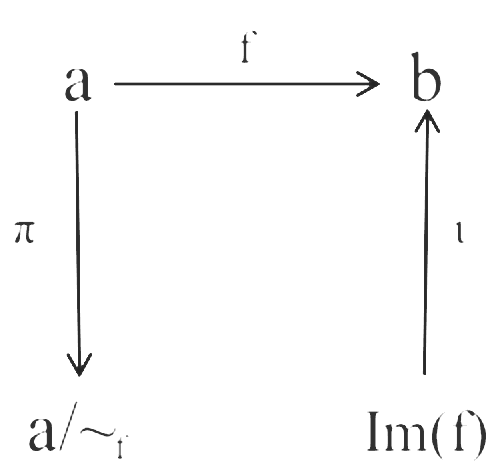
\includegraphics[scale=.2]{img/tfo1.png}

    Dati due insiemi $a$ e $b$ ed un'applicazione $f: a \to b$, possiamo costruire il seguente diagramma, dove $\pi$ è la proiezione canonica rispetto al nucleo di equivalenza di $f$ e $\iota$ (iota) è l'immersione dell'immagine nel codominio. 

    Vogliamo chiudere il diagramma, dunque definiamo:
    $$\tilde f: [x]_{\sim_f} \in a / \sim_{f}\ \mapsto\ f(x) \in Im(f)$$
    $\tilde f$ è una funzione ben posta o solo una corrispondenza? Per essere un'applicazione, per ogni classe di equivalenza deve esistere una sola immagine. Se quindi il valore $\tilde f([x]_{\sim_f})$ variasse in base a quale $z \in [x]_{\sim_f}$ scegliessimo, non sarebbe un'applicazione. Ma per definizione di nucleo di equivalenza:
    $$\forall [x]_{\sim_f} \in a / \sim_f\ \forall z, w \in [x]_{\sim_f}\ (f(z) = f(w))$$
    Allora si ha che tutti gli elementi della classe di equivalenza hanno la stessa immagine per $f$ e dunque $\tilde f$ è un'applicazione ben posta. Possiamo quindi chiudere il diagramma:

    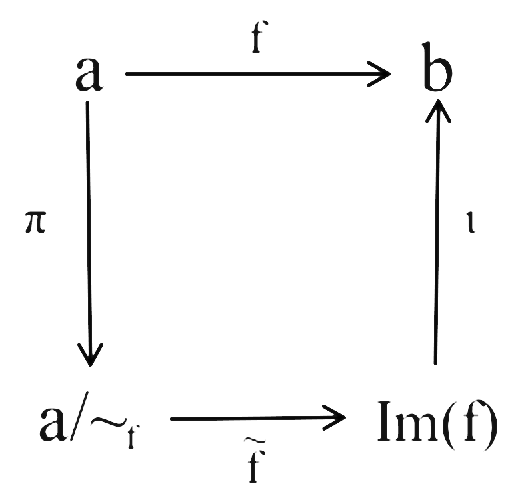
\includegraphics[scale=.2]{img/tfo2.png}
}

\subsection{Prima tesi del Teorema Fondamentale di Omomorfismi per Insiemi}
\bottom{
    $$\tilde f: [x]_{\sim_f} \in a / \sim_{f}\ \mapsto\ f(x) \in Im(f) \text{ è biettiva} $$
}
\bottomp{
    Definiamo $$\alpha: f(x) \in Im(f) \mapsto [x]_{\sim_f} \in a/\sim_f$$
    Questa è una funzione ben posta per la definizione di nucleo di equivalenza, in quanto tutte le $x$ con la stessa $f(x)$ fanno parte della stessa classe di equivalenza.
    Sia $y \in a/\sim_f$. Per le proprietà fondamentali delle classi di equivalenza $$\exists x \in a\ (y = [x]_{\sim_f})$$
    Per tanto $\alpha$ è suriettiva.

    Dalla definizione di nucleo di equivalenza $\tilde f$
    $$\forall x, y \in a\ (f(x) = f(y) \iff [x]_{\sim_f} = [y]_{\sim_f})$$
    Pertanto $\alpha$ è iniettiva.

    $\alpha$ è biettiva, $\tilde f$ è la sua inversa, quindi è anch'essa biettiva.
}

\subsection{Seconda tesi del Teorema Fondamentale di Omomorfismi per Insiemi}
\bottom{
    $$f = \iota \circ \tilde f \circ \pi$$
}
\bottomp{
    Due funzioni coincidono se hanno stesso dominio, stesso codominio, e stesso grafico.
    $$f: a \to b$$
    $$\iota \circ \tilde f \circ \pi: a\ \to\ a/\sim_f \to Im(f)\ \to\ b$$
    Hanno stesso dominio e codominio.
    $$\forall x \in a\ (\iota \circ \tilde f \circ \pi(x) = \iota(\tilde f(\pi(x))) = \iota(\tilde f([x]_{\sim_f})) = \iota(f(x)) = f(x))$$
    Anche i grafici sono identici e dunque le due funzioni sono coincidenti.
}

\subsection{Ogni Funzione è Composizione di una Funzione Iniettiva e di una Funzione Suriettiva}
\bottomp{
    Dalla $2^a$ Tesi del Teorema Fondamentale di Omomorfismo per Insiemi:
    $$\forall f\ (f = \iota \circ \tilde f \circ \pi)$$

    \(\iota\) è iniettiva, \(\tilde f\) è biettiva, e \(\pi\) è suriettiva. Pertanto possiamo esprimere \(f = (\iota \circ \tilde f) \circ \pi\) oppure \(f = \iota \circ (\tilde f \circ \pi)\). In entrambi i casi abbiamo la tesi.
}

\section{Teorema Fondamentale dell'Aritmetica}
\subsection{Lemma sui Divisori dei Primi}
\bottom{
    Se $p\in \mathbb Z$ è primo, allora $$\{n\in \mathbb Z\ |\ n|p\}=\{-1,1,p,-p\}$$
Cioè un numero primo è divisibile solo dalle unità, se stesso ed il proprio opposto.
}
\bottomp{
    Sia $n\in \mathbb Z$ tale che $$n|p\iff(\exists k\in \mathbb Z\ (nk=p\implies p|n\lor p|k))$$ (questo per la definizione di primo dato che $p|nk$ perchè $p=nk$).

Nel caso $$p|n\iff \exists h\in \mathbb Z\ (ph=n) \implies phk=nk\implies phk=p\implies hk=1$$
Allora $$(h=k=1)\lor (h=k=-1)\implies n=\pm p$$
Nel caso $$p|k\iff \exists h\in \mathbb Z\ (ph=k) \implies nph=nk\implies nph=p\implies nh=1$$
Allora $$(n=h=1)\lor (n=h=-1)\implies n=\pm 1$$
}

\subsection{Secondo Lemma per il Teorema Fondamentale dell'Aritmetica}
\bottom{
    Siano $a,b\in \mathbb N\smallsetminus \{0\}$ e sia $$x=\{n\in\mathbb N\smallsetminus \{0\}\ |\  a|nb\}$$
    Allora $\forall n \in x\ (min(x) | n)$
}
\bottomp{
    Per assurdo, sia non vuoto l'insieme degli elementi di $x$ non divisibili per il minimo e sia $z$ il minimo di tale insieme.

    Poniamo $m=min(x)$. Essendo $$z, m \in x \implies a | zb \land a | mb \implies \exists h, k \in \mathbb N\ (ah = zb \land ak = mb)$$
    Dunque
    $$a(h - k) = ah - ak = zb - mb = (z - m)b \implies a |(z - m)b$$
    Quindi $z-m\in x$, ma $z-m<z$, e $z$ era stato ipotizzato il minimo degli elementi non divisibili da $m$, il che implica che $$m|(z-m)\iff\exists l\ (ml=z-m)\implies m(l+1)=z\implies m|z$$ che è assurdo.
}

\subsection{Lemma sui divisori dei non primi}
\bottom{
    $\forall m\in\mathbb Z$ non primo ha divisori oltre $\pm 1,\pm m$.
}
\bottomp{
    $$m\in \mathbb N \text{ non primo } \iff \exists h,k\ (m|hk\land\ m\not|h\land m\not| k)$$
    Per assurdo, ipotizziamo che $$\{n\in\mathbb N\ |\ n|m\}=\{1,m\}$$
    cioè che $m$ sia divisibile solo dall'1 e sé stesso. Sia 
    $$x=\{n\in\mathbb N\smallsetminus\{0\}\ |\ m|nk\}$$ e sia $s=min(x)$.
    Dato che $h,m\in x$, per il Secondo Lemma $$s|h\land s|m$$
    ma per ipotesi solo 1 ed m sono divisori di m, quindi $$s=1\lor s=m$$
    Se $$s=1\implies m|1k \implies m|k$$che va contro l'ipotesi. Se $$s=m\implies m|h$$ (perchè per il secondo Lemma $s|h\land s|m$) che va contro l'ipotesi. In entrambi i casi abbiamo l'assurdo e quindi $m\in\mathbb Z$ ha divisori oltre $\pm1,\pm m$.
}

\subsection{2 è Primo}
\bottomp{
    $$\text{2 è primo } \iff \forall a,b\in\mathbb N\ (2|ab\implies 2|a\lor 2|b)$$
    Supponiamo che $2\not|a$ dimostriamo che necessariamente $2|b$.
    $$2|ab\ \land\ 2\not|a \implies\exists k\in\mathbb N\ (2k=ab)\ \land\ \exists h\in\mathbb N\ (a=2h+1)^*\implies2k=2hb+b$$
    E dunque $$2k-2hb=b\implies 2(k-hb)=b\implies 2|b$$ che è la tesi.\\
    (* perchè $a$ non è pari, dato che $2\not|a$).
}

\subsection{Prima Tesi del Teorema fondamentale dell'Aritmetica}
\bottom{
    Sia $m\in \mathbb Z\smallsetminus\{-1,0,1\}$, allora $\exists p_1,p_2,\dots,p_n\in\mathbb Z$ primi tali che $m=p_1\cdot p_2\cdot\dots\cdot p_n$
}
\bottomp{
    Dimostriamo tramite principio di seconda forma.

    \textbf{Caso base:} abbiamo dimostrato che 2 è primo, quindi vale per esso la tesi induttiva. Ipotizzo quindi che la tesi valga $\forall n\in\mathbb N\ (2\leq n<m)$.

    Se $m$ è primo, la tesi è provata banalmente.

    Se $m$ non è primo, allora, per il Lemma sui Divisori dei non Primi 
    $$\exists a,b\in\mathbb N\smallsetminus\{0,1,m\}\ (m=ab)$$
    e quindi si ha che $1<a,b<m$.
    Quindi per ipotesi induttiva: $$(\exists t, u \in \mathbb N)\ (\exists p_1, \dots , p_t, p_{t+1}, \dots, p_{t+u} \in \mathbb N)$$ $$(a = p_1 \cdot\ \dots\ \cdot p_t\ \land\ b = p_{t+1} \cdot \dots \cdot p_{t+u})$$
    e dunque $$m = a \cdot b = p_1 \cdot\ \dots\ \cdot p_t \cdot p_{t+1} \cdot\ \dots\ \cdot p_{t+u}$$
    e la tesi induttiva è dimostrata, e dunque essa vale $(\forall n \in \mathbb N)(n \geq 2)$.

    Considerando $m\in\mathbb Z\smallsetminus\mathbb N$. Allora $-m\in\mathbb N$ e vale per esso la tesi
    $$\exists p_1,\dots, p_r\ (-m = p_1 \cdot\ \dots\ \cdot p_r) \implies m = -(p_1 \cdot\ \dots\ \cdot p_r) = -p_1 \cdot\ \dots\ \cdot -p_r$$
    Dato che l'opposto di un numero primo è ancora un numero primo, allora la tesi vale in tutto $\mathbb Z$
}

\subsection{Seconda Tesi del Teorema Fondamentale dell'Aritmetica}
\bottom{
    Se $m = q_1 \cdot\ \dots\ \cdot q_n$ allora $r=s$ ed $\exists f: \{1,\ \dots\ , r\} \to \{1,\ \dots\ , r\}$ biettiva tale che $\forall i \in \{1,\ \dots\ , r\}\ (p_i = q_{f(i)})$
}
\bottomp{
    Dimostriamo per Principio di Induzione di Prima Forma.

    \textbf{Caso base:} $r=1$. Sia 
    $$p_1=m=q_1\cdot\ \dots\ \cdot q_s$$
    Quindi m è primo, e quindi
    $$\forall q \in \{q_1,\ \dots\ , q_s\}\ (q|m \implies q \in \{-1, 1, -m, m\}) \implies$$
    $$\implies (r = s = 1)\ \land\ (q_1 = p_1)$$
    Ora ipotizziamo che la tesi sia vera per $r-1$. Dimostriamo che è vera per r. Abbiamo che $$p_1 \cdot p_2 \cdot\ \dots\ \cdot p_r = m = q_1 \cdot q_2 \cdot\ \dots\ \cdot q_r$$
    Allora $$p_1 | q_1 \cdot q_2 \cdot\ \dots\ \cdot q_r$$
    e per la definizione di primo allora
    $$p_1 | q_1\ \lor\ p_1 | q_2\ \cdot\ \dots\ \cdot q_r$$
    Ancora una volta, per la definizione di primo
    $$p_1 | q_2 \lor p_1 | q_3 \cdot\ \dots\ \cdot q_r$$
    e così via. Dunque sia ha che 
    $$p_1 | q_1\ \lor\ p_1 | q_2 \lor\ \dots\ \lor\ p_1 | q_s$$
    Suppongo senza ledere la generalità che $p_1|q_1$. Essendo $q_1$ primo, allora $q_1=\pm p_1$(in quanto $q_1$ è divisibile solo da $\pm1,\pm q_1$, ed essendo $p_1$ primo a sua volta non può essere $\pm1$).
    Abbiamo dunque che 
    $$p_1 \cdot p_2 \cdot\ \dots\ \cdot p_r = (\pm p_1) \cdot q_2 \cdot\ \dots\ \cdot q_s$$
    E dunque cancellando $p_1$ da entrambi i membri:
    $$p_2 \cdot\ \dots\ \cdot p_r = \pm q_2 \cdot\ \dots\ \cdot q_s$$
    Siamo dunque nel caso $r-1$ e quindi vale in esso la tesi induttiva, cioè
    $$r - 1 = s - 1\ \land\ (\exists \sigma: \{2, ..., r\} \to \{2, ..., r\} \text{ biettiva})$$$$ \forall i \in \{2, ..., r\}\ (p_i = \pm q_{\sigma(i)})$$
    Basta quindi definire:
    $$f: i \in \{2, ..., r\} \mapsto 
    \begin{cases}
    \sigma(i) &i \in \{2, ..., r\}\\
    1 &i = 1\\
    \end{cases}$$
    Per avere la tesi.
}
\section{Insiemi Ordinati}
\subsection{Insieme delle Relaioni d'Ordine}
\bottom{
    Dato $a$, allora definiamo gli insiemi:
    \begin{align*}
        &OL(a) = \{\rho \in P(P(P(a \times a))) \mid \rho \text{ riflessiva, asimmetrica, transitiva}\}\\
        &OS(a) = \{\rho \in P(P(P(a \times a))) \mid \rho \text{ antiriflessiva, asimmetrica, transitiva}\}
    \end{align*}
}

\subsection{Le relazioni appartengono a \texorpdfstring{$P(P(P(a \times a)))$}{PPPaa}}
\bottomp{
    Consideriamo la relazione
    $$\rho = (a \times a, g) = \{\{a \times a\}, \{a\times a, g\}\}$$
    \begin{align*}
        &&&a \times a \subseteq a \times a \implies a \times a\ \in P(a \times a)\\
        &&&g \subseteq a \times a \implies g \in P(a \times a)\\
        &\text{Questo implica che}\\
        &&&\{a \times a\} \in P(P(a \times a))\\
        &&&\{a \times a, g\} \in P(P(a \times a))\\
        &\text{E dunque}\\
        &&&\{\{a \times a\}, \{a \times a, g\}\} \in P(P(P(a \times a)))
    \end{align*}
}

\subsection{DA \texorpdfstring{\textit{OL}}{OL} a \texorpdfstring{\textit{OS}}{OS} e viceversa}
\bottom{
    \begin{align*}
        &\text{Sia } \rho \in OL(a)\text{, definisco}\\
        &&&\rho^\land :\Leftrightarrow (\forall x, y \in a)(x \rho^\land y \iff (x \rho y \land x \neq y))\\
        &\text{Sia } \rho \in OS(a)\text{, definisco}\\
        &&&\rho^\lor :\Leftrightarrow (\forall x, y \in a)(x \rho^\lor y \iff (x \rho y \lor x = y))
    \end{align*}
    Si dimostra che $$f: \rho \in OL(a) \mapsto \rho^\land \in OS(a)$$ è biettiva e la sua inversa è $$f^{-1}: OS(a) \mapsto \rho^\lor \in OL(a)$$
    Pertanto, per ogni relazione d'ordine stretto esiste una corrispondente relazione d'ordine largo e viceversa.
}

\subsection{Insieme Ordinato}
\bottom{
    Sia $s\not=\emptyset$ e sia $\rho$ una relazione d'ordine su $s$. La coppia $(s,\rho)$ si dice insieme ordinato.
}

\subsection{Relazione d'ordine Indotto}
\bottom{
    Sia $(s,\rho)$ un insieme ordinato e sia $t\subseteq s$. Definiamo relazione d'ordine indotto da $(s,\rho)$ su $t$ la relazione d'ordine:
$$\rho_t = (t \times t, g_\rho \cap (t \times t))$$
}

\subsection{Sottoinsieme Ordinato}
\bottom{
    Dato un'insieme ordinato \((s, \rho)\) e dato \(t \subseteq s\) e \(\rho_t\) la relazione d'ordine indotta da \((s, \rho)\) su \(t\), allora definiamo \((t, \rho_t)\) sottoinsieme ordinato di \((s, \rho)\).
}

\subsection{Elementi Confrontabili}
\bottom{
    Dato un insieme ordinato \((s, \rho)\), due elementi \(x, y \in s\) si dicono confrontabili $\iff$ 
    $$x \rho y \lor y \rho x$$
}

\subsection{Relazione d'Ordine Totale}
\bottom{
    Data una relazione d'ordine \((s, \rho)\), se ogni elemento di \(s\) è confrontabile, allora \(\rho\) si dice relazione d'ordine totale e \((s, \rho)\) si dice insieme totalmente ordinato.
}

\subsection{Minimo e Massimo di un Insieme Ordinato}
\bottom{
    Dato un insieme ordinato \((s, \rho)\) allora:

    $$ m \in s \text{ massimo di } s :\iff \forall x \in s\ (x \rho m) $$
    $$ m \in s \text{ minimo di } s :\iff \forall x \in s(m \rho x) $$
}

\subsection{Insieme Ben Ordinato}
\bottom{
    Un insieme ordinato \((s, \rho)\) si dice ben ordinato se ogni suo sottoinsieme non vuoto (incluso sé stesso) è dotato di minimo.
}

\subsection{Unicità di Minimi e Massimi di un Insieme Ordinato}
\bottom{
    Se esiste minimo e/o massimo in un insieme ordinato \((s, \rho)\) allora essi sono unici.
}
\bottomp{
    Dimostriamo per il minimo, il caso del massimo è del tutto analogo. 
    \begin{align*}
        &&&Siano\ m_1, m_2 \in s\ minimi\ di\ s.\\
        &\text{Per definizione di minimo:}\\
        &&&\forall x \in s\ (m_1 \rho x)\ \land\ \forall x \in s\ (m_2 \rho x)\\
        &\text{Per l'asimmetria di } \rho \text{ segue:}\\
        &&& (m_1 \rho m_2\ \land\ m_2 \rho m_1) \implies m_1 = m_2
    \end{align*}
}

\subsection{Notazione di Minimo e Massimo di un Insieme}
\bottom{
    Essendo minimo e massimo di un insieme $t$ unici li noteremo come $max(t)$ e $min(t)$.
}

\subsection{Buon Ordine implica Ordine Totale}
\bottom{Se \((s, \rho)\) è un insieme ben ordinato, allora esso è anche totalmente ordinato.}
\bottomp{
    $$\forall x, y \in s$$
    $$ \exists n \in \{x, y\}$$
    $$ n = min(\{x, y\}) \implies n = x \lor n = y \implies x \rho y \lor y \rho x$$
}

\subsection{Relazione di Copertura}
\bottom{
    Dato un insieme ordinato \((s, \rho)\) ed \(x, y \in s\) diremo che:

    \(y \text{ COPRE } x :\iff x \rho y\ \land\ \nexists z \in s\ (z \neq x\ \land\ z \neq y\ \land\ x \rho z\ \land z \rho y)\)
}

\subsection{Predecessore/Successore Immediato}
\bottom{
    Dato un insieme ordinato \((s, \rho)\) e \(x, y \in s\) tale che \(y\) copre \(x\), allora diremo che \(y\) è l'immediato successore di \(x\) e che \(x\) è l'immediato predecessore di \(y\).
}

\subsection{Diagramma di Hasse}
\bottom{
    Dato un insieme ordinato \((s, \rho)\) definiremo il suo diagramma di Hasse la coppia \((s \times s, g)\) tale che 
    $$\forall x, y \in s\ \ (x, y) \in g \iff y \text{ COPRE } x$$
}

\subsection{Rappresentazione Grafica del Diagramma di Hasse}
\bottom{
    Dato un insieme ordinato \((s, \rho)\) su cui definiamo un diagramma di Hasse, lo rappresenteremo graficamente assegnando ad ogni elemento di \(s\) un vertice, connettendo due vertici con un lato solo se uno copre l'altro, con il vertice che copre piazzato più in alto rispetto a quello coperto.
}

\subsection{Ordine Totale e Diagrammi di Hasse}
\bottom{
    Si osserva che se l'insieme è totalmente ordinato, il suo diagramma di Hasse è una linea.
}

\subsection{Funzione Crescente fra Insiemi Ordinati}
\bottom{
    Dati due insiemi ordinati \((s, \rho)\) e \((\Bar{s}, \Bar{\rho})\), diremo che la funzione \(f: s \to \Bar{s}\) è crescente \(:\iff\)
    $$ \forall x, y \in s\ (x \rho y \implies f(x)\ \Bar{\rho}\ f(y))$$
}

\subsection{Isomorfismo di Insiemi Ordinati}
\bottom{
    Dati due insiemi ordinati \((s, \rho)\) e \((\Bar{s}, \Bar{\rho})\), diremo che la funzione \(f: s \to \Bar{s}\) è isomorfismo \(:\iff\)
    $$ \forall x, y \in s\ (x \rho y \iff f(x)\ \Bar{\rho}\ f(y))$$
}

\subsection{Insiemi Ordinati Finiti sono Isomorfi solo se hanno lo stesso Diagramma di Hasse }
\bottom{
    Siano \((s, \rho)\) e \((\Bar s, \Bar \rho)\) due insiemi ordinati finiti e sia \(f: s \to \Bar s\) un isomorfismo \(\iff\) hanno lo stesso Diagramma di Hasse
}

\subsection{Minimali e Massimali di un Insieme Ordinato}
\bottom{
    Dato un insieme ordinato \((s, \rho)\) e un suo sottoinsieme ordinato \(t \subseteq s\), diremo che:

    \(m \in s \text{ massimale di } t :\iff\)
    $$ \forall x \in t\ (x \rho m \lor m \rho x \implies x \rho m)$$
    \(m \in s \text{ minimale di } t :\iff\)
    $$ \forall x \in t\ (x \rho m \lor m \rho x\implies m \rho x)$$

    Cioè un elemento è massimale (o minimale) solo se è più grande (o più piccolo) di ogni elemento con cui è confrontabile.
}
\subsection{Maggioranti e Minoranti di un Insieme Ordinato}
\bottom{
    Dato un insieme ordinato \((s, \rho)\) e un suo sottoinsieme ordinato \(t \subseteq s\), diremo che:

    \(m \in s \text{ maggiorante di } t :\iff\)
    $$\forall x \in t\ (x \rho m)$$
    \(m \in s \text{ minorante di } t :\iff\)
    $$ \forall x \in t\ (m \rho x)$$

    Cioè un elemento di \(s\) è maggiorante (o minorante) solo se è più grande (o più piccolo) di ogni elemento di \(t\).
}

\subsection{Relazione fra Massimali/Maggioranti/Massimi e Minimali/Minoranti/Minimi}
\bottom{
    \begin{align*}
    &\text{massimo} \implies \text{maggiorante} \implies \text{massimale} \\
    &\text{minimo} \implies \text{minorante} \implies \text{minimale}
    \end{align*}
}

\subsection{Notazione di Insieme dei Maggioranti e di Insieme dei Minoranti}
\bottom{
    Dato un insieme ordinato \((s, \rho)\) e un suo sottoinsieme ordinato \(t \subseteq s\). Allora noteremo:
    \begin{align*}
        &MAGGIOR_{(s, \rho)}(t) := \text{ insieme dei maggioranti di } t \text{ in } s\\
        &MINOR_{(s, \rho)}(t) := \text{ insieme dei minoranti di } t \text{ in } s
    \end{align*}
}

\subsection{Insieme Limitato}
\bottom{
    Sia \((s, \rho)\) un insieme ordinato e \(t \subseteq s\). Allora:
    \begin{align*}
        &t \text{ è limitato inferiormente } :\iff MINOR_{(s, \rho)}(t) \neq \emptyset\\
        &t \text{ è limitato superiormente } :\iff MAGGIOR_{(s, \rho)}(t) \neq \emptyset
    \end{align*}

    Cioè se è dotato di minorante e/o maggiorante.
}

\subsection{Insieme Naturalmente Ordinato}
\bottom{
    \((s, \rho)\) insieme ordinato è naturalmente ordinato \(:\iff\) è ben ordinato e ogni sua parte non vuota superiormente limitata ha massimo.
}

\subsection{Il buon ordine implica l'ordine largo}
\bottomp{
    Sia \((s, \rho)\) un insieme ben ordinato. Allora:

    $$\forall x \in s\ (\{x\} \text{ ha minimo } \implies x \rho x)$$
}

\subsection{Assioma dei Numeri Naturali}
\bottom{
    Esiste un insieme naturalmente ordinato non limitato superiormente e questo insieme è \(\mathbb{N}\). Questo assioma è equivalente all'Assioma dell'Infinito.
}

\subsection{Principio di Dualità per Insiemi Ordinati}
\bottom{
    Dato \((s, \rho)\) e la duale \(\overline\rho\), allora si osserva che:
    \(max(s, \rho) = min(s, \overline\rho)\)
    Cioè, ogni massimo è minimo per la duale, e ogni minimo è massimo per la duale.
    Quindi, se dimostriamo un teorema per il massimo, allora esso varrà anche per il minimo (cioè il massimo della duale), e viceversa.
}

\subsection{Il Minimo (Massimo) è l'unico Minimale (Massimale)}
\bottom{
    Dato un insieme ordinato \((s, \rho)\) con \(m = min(s, \rho)\), allora esso è l'unico minimale interno ad \((s, \rho)\) (per dualità, lo stesso vale per il massimo).}
    \bottomp{Sia \(n \in s\) minimale di \((s, \rho)\). Per definizione di minimo, si ha che \(m \rho n\). Ma questo vuol dire che \(m, n\) sono confrontabili, quindi per definizione di minimale \(n \rho m\). Per asimmetria, allora i due coincidono.
}

\subsection{Ogni Insieme Ordinato Finito Non Vuoto di Ordine Largo ha Minimali e Massimali}
\bottom{
    $$(s, \rho) \land \rho \in OL(s) \implies (s, \rho) \text{ ha minimali} \in s$$
    Per dualità, allora ha anche massimali.}
\bottomp{
    Sia \(x \in s\). Per assurdo, ipotizziamo che \((s, \rho)\) non abbia minimali, e dunque \(x\) non è un minimale. Se \(s = \{x\}\), allora \(x\) sarebbe minimale, il che è assurdo. Quindi \(s \neq \{x\}\). Ipotizziamo che \(s\) sia di due elementi. Allora \(\exists y \in s\ (x \neq y)\). Ma \(y\), per ipotesi di assurdo, non è minimale. Quindi si deve avere che \(x \rho y\), ma ciò implicherebbe che \(x\) è minimale. Pertanto, deve \(\exists z \in s\ (z \neq x \land z \neq y)\). Ma per ipotesi di assurdo, \(z\) non è minimale, quindi si deve avere che \(x\rho z \lor y \rho z\), ma questo implicherebbe che uno di loro è minimale. Allora deve esistere un elemento \(w\)... ma chiaramente questo continua all'infinito, e \(s\) è un insieme finito. Pertanto, c'è l'assurdo e deve esistere un minimale.
}

\subsection{In Insiemi Finiti l'unico Minimale (Massimale) è Minimo (Massimo)}
\bottom{
    Questo non vale per gli insiemi infiniti.
}

\subsection{Relazione d'Ordine Indotta da una Funzione}
\bottom{
    Sia \(f: a \to b\) e sia \(\rho \in OL(b)\). Allora definiamo la relazione \(\rho_f\) tale che:

    $$\forall x, y \in a\ (x \rho_f y \iff f(x) \rho f(y))$$

    la relazione d'ordine indotta da \(f\) su \(a\).
}

\subsection{Estremo Superiore ed Estremo Inferiore}
\bottom{
    Sia \((s, \rho)\) un insieme ordinato e \(t \subseteq s\). Definiamo l'estremo inferiore e l'estremo superiore rispettivamente:

    $$SUP_{(s, \rho)}(t) = min(MAGGIOR_{(s, \rho)}(t)) \text{ (se esiste)}$$
    $$INF_{(s, \rho)}(t) = max(MINOR_{(s, \rho)}(t)) \text{ (se esiste)}$$
}








\section{Reticoli}
\subsection{Reticolo}
\bottom{
    Sia \((s, \rho)\) un insieme ordinato, con \(\rho \in OL(s)\). Allora:
    \((s, \rho)\) è un reticolo \(:\iff\) $$\forall x,y \in s$$
    $$ \exists z, w \in s$$ $$ z = INF_{(s, \rho)}(\{x, y\}) \land w = SUP_{(s, \rho)}(\{x, y\})$$

    Cioè l'insieme di ogni coppia di elementi di \(s\) è dotato di estremo superiore ed inferiore in \(s\).
}

\subsection{Operazioni in un Reticolo}
\bottom{
        Dato un reticolo $(s, \rho)$, possiamo definire, \(\forall x, y \in s\):
    \begin{align*}
        &\text{Intersezione reticolare}\\
        &&&\wedge: (x, y) \in s \times s \mapsto INF_{(s, \rho)}(\{x, y\}) \in s\\
        &\text{Unione Reticolare}\\
        &&&\vee: (x, y) \in s \times s \mapsto SUP_{(s, \rho)}(\{x, y\}) \in s
    \end{align*}
    Cioè due operazioni binarie ed interne.
}

\subsection{Notazione di Reticolo come Struttura}
\bottom{
    Dato un reticolo \((s, \rho)\), dato che possiamo definire in esso due operazioni binarie interne \(\vee\) e \(\wedge\), allora possiamo notarlo come una struttura: \((s, \wedge, \vee)\)
}

\subsection{Reticolo Limitato}
\bottom{
    Un reticolo \((s, \rho)\) si dice limitato se è dotato di minimo e massimo.
}

\subsection{Reticolo Completo}
\bottom{
    Un reticolo \((s, \rho)\) si dice completo se ogni sua parte non vuota è dotata di estremi superiore ed inferiore.
    Ogni reticolo completo è anche un reticolo limitato.
}

\subsection{Estremi di Coppie di Elementi Confrontabili di un Reticolo}
\bottom{
    Dato un reticolo \((s, \rho)\) e due elementi \(x, y \in s\). Siano essi confrontabili, ad esempio \(x \rho y\). Allora:

    $$INF_{(s,\rho)}(\{x, y\}) = (x \wedge y) = x$$
    $$SUP_{(s,\rho)}(\{x, y\}) = (x \vee y) = y$$
}
\bottomp{
    \(x \rho x\) per riflessività di \(\rho\) (che, essendo \(s\) un reticolo, deve necessariamente essere d'ordine largo). Per ipotesi, \(x \rho y\). Dunque \(x\) è minimo di \(\{x, y\}\), e quindi è anche estremo inferiore.
    Analgoamente si dimostra per l'estremo superiore.
}

\subsection{Enunciato Duale sui Reticoli}
\bottom{
    Sia \((s, \rho)\) un reticolo, e \((s, \overline\rho)\) il suo reticolo duale. Se \(e\) è un enunciato sui reticoli, dico enunciato duale \(\overline e\) l'enunciato ottenuto:

    - Rimpiazzando ogni \(\rho\) in \(e\) con \(\overline \rho\) (e viceversa)

    - Rimpiazzando ogni \(\wedge\) in \(e\) con \(\vee\) (e viceversa)
}

\subsection{Principio di Dualità Per i Reticoli}
\bottom{
    Se \(e\) è una formula valida per ogni reticolo, allora anche la sua duale \(\overline e\) lo è.
}
\bottomp{
    \(e\) è valida per ogni reticolo \((s, \rho)\), ma quindi è valida anche per il suo duale \((s, \overline\rho)\). Ma nel reticolo duale, gli estremi inferiori sono estremi superiori e viceversa. Dunque, \(e\) riferito a \((s, \overline\rho)\) è esattamente \(\overline e\) riferito a \((s, \rho)\).
}

\subsection{In un Reticolo ogni Minimale è Minimo e ogni Massimale è Massimo}
\bottomp{
    Dimostriamo per i minimali, per dualità vale anche per i massimali.

    Sia \((s, \rho)\) un reticolo e sia \(m \in s\) minimale. Sia \(x \in s\) un elemento generico del reticolo. Allora si ha che $$(m \wedge x)\ \rho\ m$$ per la definizione di estremo inferiore. Ma quindi \(m \wedge x\) ed \(m\) sono confrontabili, e dunque per la definizione di minimale, $$m\ \rho\ (m \wedge x)$$ Dunque per asimmetria \(m \wedge x = m\), per ogni \(x \in s\), e allora \(m\) è mimimo di \(s\).
}

\subsection{In un Reticolo I Minoranti (Maggioranti) dell'Unione sono l'Intersezione dei Minoranti (Maggioranti) di Parti Finite}
\bottom{
    Sia \((s, \rho)\) un reticolo e siano \(a, b \in P(s)\) finiti. Allora:
$$MINOR_{(s, \rho)}(a \cup b) = MINOR_{(s, \rho)}(a) \cap MINOR_{(s, \rho)}(b)$$
Per dualità vale l'analogo per i maggioranti.
}
\bottomp{
    \begin{align*}
        x \in MINOR_{(s, \rho)}(a \cup b) &\iff \forall y \in a \cup b\ (x \rho y)  \\
        &\iff \forall y\ (y \in a \lor y \in b \implies x \rho y)  \\
        &\iff \forall y\ (y \in a \implies x \rho y) \land \forall y\ (y \in b \implies x \rho y) \\
        &\iff x \in MINOR_{(s, \rho)}(a) \land x \in MINOR_{(s, \rho)}(b) \\
        &\iff x \in MINOR_{(s, \rho)}(a) \cap MINOR_{(s, \rho)}(b) 
    \end{align*}
}

\subsection{I Minoranti (Maggioranti) di un Insieme Ordinato sono i Minoranti (Maggioranti) dell'Estremo Inferiore (Superiore)}
\bottom{
    Sia \((s, \rho)\) un insieme ordinato e sia \(a \subseteq s\). Se esiste \(m = INF_{(s,\rho)}(a)\), allora:

    $$MINOR_{(s,\rho)}(a) = MINOR_{(s,\rho)}(\{m\})$$
}
\bottomp{
    Questo deriva semplicemente dal fatto che l'estremo inferiore è il massimo dei minoranti.
}

\subsection{Ogni Parte Finita di un Reticolo è dotata di Estremi Inferiore e Superiore}
\bottom{
    Sia \((s, \rho)\) un reticolo. Ogni sua parte finita è dotata di estremo inferiore e superiore.
}
\bottomp{
    Siano \(a, b \in P(s)\) due insiemi finiti. Allora:
    1) Per "I Minoranti (Maggioranti) dell'Unione sono l'Intersezione dei Minoranti (Maggioranti) degli Insiemi Finiti" e per "I Minoranti (Maggioranti) di un Insieme sono i Minoranti (Maggioranti) dell'Estremo Inferiore (Superiore)" abbiamo che:

    Siano $$m_1 = INF_{(s, \rho)}(a)$$
    $$ m_2 = INF_{(s, \rho)}(b)$$
    \begin{align*}
        &MINOR_{(s, \rho)}(a \cup b) =\\
        & MINOR_{(s, \rho)}(a) \cap MINOR_{(s, \rho)}(b) =\\
        & MINOR_{(s, \rho)}(\{m_1\}) \cap MINOR_{(s, \rho)}(\{m_2\}) =\\
        &MINOR_{(s, \rho)}(\{m_1, m_2\})
    \end{align*}

    2) Dimostriamo per induzione su \(n = |t|\) dove \(t\) è una parte finita di \(s\).
    Caso base: \(n = 1\). Allora \(t\) è un singleton, ed il suo unico elemento è (per riflessività) sia estremo superiore che estremo inferiore.
    Assumendo adesso che la tesi induttiva sia valida per ogni \(1 \leq k < n\), dimostriamo per \(n\).
    Sia \(x \in t\). Allora $$t = (t - \{x\}) \cup \{x\}$$ cioè l'unione di un insieme di ordine \(n-1\) e di uno di ordine \(1\). Per ipotesi induttiva, allora essi sono dotati di estremi inferiori, con $$m = INF_{(s, \rho)}(t - \{x\})$$
    $$ x = INF_{(s, \rho)}(\{x\})$$
    Allora, per la (1):
    $$
    MINOR(t) = MINOR((t - \{x\}) \cup x) = MINOR(\{m, x\}).
    $$

    Dato che siamo in un reticolo, la coppia \(\{m, x\}\) ha sicuramente estremo inferiore, cioè massimo di $$MINOR(\{m, x\}) = MINOR(t)$$ da cui la tesi.

    Per dualità, lo stesso vale per l'estremo superiore.
}

\subsection{Commutatività di \(\wedge\) e \(\vee\)}
\bottom{
    Sia \((s, \wedge, \vee)\) un reticolo. Allora:
    $$\forall x, y \in s\ ((x \wedge y = y \wedge x) \land (x \vee y = y \vee x))$$
}
\bottomp{
    $$x \wedge y = INF_{(s, \rho)}(\{x, y\}) = INF_{(s, \rho)}(\{y, x\}) = y \wedge x$$
    $$x \vee y = SUP_{(s, \rho)}(\{x, y\}) = SUP_{(s, \rho)}(\{y, x\}) = y \vee x$$
}

\subsection{Associatività di \(\wedge\) (Wedge) e \(\vee\) (Vee)}
\bottom{Sia \((s, \wedge, \vee)\) un reticolo. Allora \(\wedge, \vee\) sono associative.}
\bottomp{
    Dimostriamo per \(\vee\), la dimostrazione per \(\wedge\) è analoga per dualità.

    Siano \(x, y, z \in s\). Per definizione abbiamo che:
    \begin{itemize}
        \item \(x \rho [x \vee (y \vee z)]\)
        \item \((y \vee z) \rho [x \vee (y \vee z)]\)
        \item  \(y \rho (y \vee z)\)
        \item \(z \rho (y \vee z)\)
    \end{itemize}

    Allora per transitività:
    $$y \rho [x \vee (y \vee z)]$$

    $$z \rho [x \vee (y \vee z)]$$

    E dunque:
    $$(x \vee y) \rho [x \vee (y \vee z)]$$

    Ed infine:
    $$[(x \vee y) \vee z] \rho [x \vee (y \vee z)]$$

    Lo stesso procedimento si può fare nel senso opposto per dimostrare che $$[x \vee (y \vee z)] \rho [(x \vee y) \vee z]$$
    Dunque, per asimmetria:
    $$[(x \vee y) \vee z] = [x \vee (z \vee y)]$$
}

\subsection{Proprietà di Assorbimento di un Reticolo}
\bottom{
    $$\forall x, y \in s\ ((x \vee (x \wedge y) = x) \land (x \wedge (x \vee y) = x))$$
}

\subsection{Proprietà di Idempotenza/Iteratività di \(\wedge\) (Wedge) e \(\vee\) (Vee)}
\bottom{
    In un reticolo \((s, \rho)\) $$\forall x  \in s\ (x = x \vee x = x \wedge x )$$
}
\bottomp{
    Dimostriamo per \(\wedge\), analogo per \(\vee\).
    Dalle proprietà di assorbimento, segue che:
    $$\forall y \in s\ (x \wedge (x \vee y) = x)$$
    Dato che \(x \wedge x \in s\), allora, ponendo \(y = x \wedge x\) e applicando ancora una volta l'assorbimento:
    $$x = x \wedge (x \vee (x \wedge x)) = x \wedge x $$
}

\subsection{Corrispondenza Biunivoca fra Reticoli e Strutture}
\bottom{
    Sia \(s\) un insieme non vuoto e sia \(r\) l'insieme delle relazioni d'ordine largo \(\rho\) per cui \(s\) è un reticolo.
    Sia \(b\) l'insieme delle coppie di operazioni binarie interne \((\alpha, \beta)\) tali che entrambe siano commutative, associative, e valga la legge di assorbimento in \((s, \alpha, \beta)\)
    Allora l'applicazione $$f: \rho \in r \mapsto (\wedge_\rho, \vee_\rho) \in b \text{ è biettiva}$$ Cioè, da ogni reticolo si possono definire wedge e vee, e ogni coppia di operazioni associative, commutative, idempotenti, e per cui vale l'assorbimento sono sono wedge e vee di un qualche reticolo.
}
\bottomp{
    Per dimostrare che \(f\) è biettiva, vogliamo trovare la sua inversa. Siano \((\wedge, \vee) \in b\) e definiamo \(\rho\) tale che $$\forall x, y \in s\ (x \rho y \iff x = x \wedge y)$$
    Nota che da questo segue che \(x \vee y = (x \wedge y) \vee y = y\) per assorbimento.

    1) \(\rho\) così definita è di ordine largo? Per idempotenza, $$x \wedge x = x \implies x \rho x$$ quindi vale la riflessività. Se $$(x = x \wedge y) \land (y = y \wedge x)$$ dato che wedge è ipotizzata commutativa, \(x = y\) e quindi vale l'asimmetria.
    Se \(x \rho y \land y \rho z\), allora $$(x = x \wedge y) \land (y = y \wedge z)$$ Quindi, per associatività: $$x = x \wedge (y \wedge z) = (x \wedge y) \wedge z = x \wedge z \implies x \rho z$$ quindi vale la transitività.
    \(\rho\) è effettivamente una relazione d'ordine largo.

    2) Vogliamo far vedere che $$INF_{(s, \rho)}(\{x, y\}) = x \wedge y$$ e che $$SUP_{(s, \rho)}(\{x, y\}) = x \vee y$$ per ogni \(x, y \in s\).
    Per assorbimento $(x \wedge y) \vee x = x$ quindi per definizione abbiamo che $(x \wedge y) \rho x$ Analogamente $(x \wedge y) \rho y$
    Quindi $$x \wedge y \in MINOR_{(s, \rho)}(\{x, y)\}$$ Vogliamo far vedere che \(x \wedge y\) è il massimo dell'insieme. Sia dunque \(z\) un generico minorante. Allora si ha:
    $$z\rho y \land z \rho x \implies (z = z \wedge y) \land (z = z \wedge x)$$
    E quindi:
    \(z = z \wedge x = (z \wedge y) \wedge x = z \wedge (x \wedge y) \implies z \rho (x \wedge y)\) da cui la tesi che \(x \wedge y\) è estremo inferiore.
    Lo stesso procedimento vale, analogamente, per gli estremi superiori.

    Si osserva semplicemente che la funzione \((\wedge, \vee) \in b \mapsto \rho \in r\) è l'inversa di \(f\), da cui la tesi.
}

\subsection{Isomorfismo fra Reticoli}
\bottom{
    Siano \((s, \wedge, \vee), (s', \wedge', \vee')\) due reticoli. Allora \(f: s \to s'\) si dice isomorfismo fra i due reticoli se:

    1) \(f\) è biettiva

    2) $\forall x, y \in s\ ((f(x \wedge y) = f(x) \wedge' f(y)) \land (f(x \vee y) = f(x) \vee' f(y)))$
}

\subsection{Equivalenza fra Isomorfismo di Reticoli e Isomorfismo di Insiemi Ordinati}
\bottom{
    Siano \((s, \wedge, \vee), (s', \wedge', \vee')\) due reticoli e sia \(f: s \to s'\) una funzione biettiva fra i due. Allora:
    \(f\) isomorfismo fra i reticoli \(\iff\) \(f\) è un isomorfismo di insiemi ordinati fra \((s, \rho_{(\wedge, \vee)})\) e \((s', \rho_{(\wedge', \vee')})\)
}
\bottomp{
    Dimostrazione \(\Leftarrow)\):

    Siano \((s, \rho), (s, \rho)\) due reticoli e sia \(f\) un isomorfismo di insiemi ordinati fra essi. I reticoli possono essere espressi come strutture \((s, \wedge_\rho, \vee_\rho), (s', \wedge_{\rho'}, \vee_{\rho'})\)

    Si ha che: $$\forall x, y \in s\ (((x \wedge_\rho y) \rho x) \land ((x \wedge_\rho y) \rho y))$$
    Applicando l'isomorfismo: $$f(x \wedge_\rho y) \rho' f(x)\text{ e } f(x \wedge_\rho' y) \rho' f(y)$$
    Quindi $$f(x \wedge_\rho' y) \in MINOR_{(s', \rho')}(\{f(x), f(y)\})$$
    Sia \(z \in MINOR_{(s', \rho')}(\{f(x), f(y)\})\).

    Si ha che $$z \rho' f(x) \text{ e } z \rho' f(y)$$
    Essendo \(f\) suriettiva, $\exists w \in s\ (f(w) = z)$.
    Allora, applicando l'isomorfismo in senso inverso $w\rho x \land w \rho y$. Quindi \(w\) è minorante di \(\{x, y\}\).
    Allora si ha che:
    $$w \rho (x \wedge_\rho y) \implies f(w) \rho' f(x \wedge_\rho y) \implies z \rho' f(x \wedge_\rho y)$$
    E quindi \(f(x \wedge_\rho y)\) è extremo inferiore di \(\{f(x), f(y)\}\), cioè:
    $$f(x \wedge_\rho y) = f(x) \wedge_{\rho'} f(y)$$ che è la tesi.
    Analogamente si dimostra per \(\vee\).

    Dimostrazione \(\Rightarrow\):
    Sia \(f\) isomorfismo fra \((s, \wedge, \vee), (s', \wedge', \vee')\) e siano \(\rho, \rho'\) le relazioni d'ordine associate.
    Prendiamo \(x, y \in s: x \rho y\). Per definizione \(x = x \wedge y\) e quindi $$f(x) = f(x \wedge y) = f(x) \wedge' f(y) \iff f(x) \rho' f(y)$$
    Questo vale in entrambi i versi (in quanto è una catena di uguaglianze seguita da un'equivalenza materiale) e quindi abbiamo la tesi.
}

\subsection{Sottoreticolo}
\bottom{
    Sia \((s, \wedge, \vee)\) un reticolo e sia \(t \in P(s) - \{\emptyset\}\). Se \(t\) è parte chiusa rispetto a \(\wedge, \vee\), esso si dice sottoreticolo di \((s, \wedge, \vee)\).
}

\subsection{Intervallo e Intervallo Chiuso}
\bottom{
    Sia \((s, \rho)\) un insieme ordinato, con \(\rho \in OL(s)\).

    \(i \subseteq s \text{ intervallo } :\iff\)
    $$ \forall x, y \in i$$
    $$ \forall z \in s$$
    $$(x\rho z \land z \rho y \implies z \in i)$$

    In particolare, se \(i\) è limitato, si dice intervallo chiuso.
}

\subsection{Ogni Intervallo Chiuso di un Reticolo è un Sottoreticolo}
\bottom{
    Se \((s, \rho)\) è un reticolo, ogni suo intervallo chiuso è un sottoreticolo.
}
\bottomp{
    Sia \(i \in s\) un sottointervallo. Allora, dati \(x, y \in i\), esiste estremo inferiore \(x \wedge y \in s\). $$min(i) \rho x \land min(i) \rho y \implies min(i) \rho (x \wedge y) \rho x \implies x \wedge y \in i$$
    Procedimento analogo si effettua per l'estremo superiore.
}

\subsection{Massimo e Minimo sono Elementi Neutri di un Reticolo (e Viceversa)}
\bottom{
    Sia \((s, \rho)\) un reticolo. Siano \(m, M \in s\). Allora:

    \(m \text{ minimo di } s \iff m \text{ neutro di } \vee_\rho\)

    \(M \text{ massimo di } s \iff M \text{ neutro di } \wedge_\rho\)
}
\bottomp{
    \(\Rightarrow)\) Sia \(x \in s\). Allora \(x \rho M \land x \rho x\). Dunque \(x = min(\{x, M\}) = x \wedge_\rho M\). Dunque \(M\) è neutro.

    \(\Leftarrow)\) \(\forall x \in s\ (m\wedge_\rho x =x) \implies \forall x \in s\ (x \rho M)\).

    Analogamente si dimostra per il minimo.
}

\subsection{Reticolo Complementato}
\bottom{
    Un reticolo limitato \((s, \rho)\) si dice complementato se:
    $$\forall x \in s,\ \exists y \in s$$
    $$ (x \wedge y = min(s) \land x \vee y = max(s))$$

    E si dice che \(x\) è complementato e che \(y\) è il suo complemento.
}


\subsection{Elementi Confrontabili e Complementati di un Reticolo sono il Minimo e il Massimo}
\bottom{
    Sia \((s, \rho)\) un reticolo complementato. Allora:
    Due elementi \(x, y \in s\) sono confrontabili e complementati \(\iff\) uno è il minimo e l'altro è il massimo.
}
\bottomp{
    Se i due elementi sono confrontabili, allora essi sono rispettivamente il minimo e massimo della loro coppia, e sono quindi anche estremo inferiore e superiore. Ma essendo i due elementi complementari, per ipotesi, allora si ha che il loro estremo inferiore è il minimo ed il loro estremo superiore è il massimo. Perciò essi coincidono.
}

\subsection{Reticolo Distributivo}
\bottom{
    Un reticolo \((s, \wedge, \vee)\) si dice distributivo se valgono entrambe le Leggi Distributive:
    $$\forall a, b, c \in s\ (a \wedge (b \vee c) = (a \wedge b) \vee (a \wedge c))$$
    $$\forall a, b, c \in s\ (a \vee (b \wedge c) = (a \vee b) \wedge (a \vee c))$$
    Si dimostra che se in un Reticolo vale una legge di distributività, allora vale anche l'altra. Dunque, per essere un reticolo distributivo, basta che valga una delle due leggi dato che l'altra segue.
}

\subsection{Unicità dei Complementi di Reticoli Distributivi}
\bottom{
    Sia \((s, \rho)\) un reticolo distributivo limitato. Allora ogni complemento è unico.
}
\bottomp{
    Sia \(x \in s\) e siano \(y, z \in s\) suoi complementi. Allora:
    $$y = y \wedge max(s) = y \wedge (x \vee z) = (y \wedge x) \vee (y \wedge z) = min(s) \vee (y \wedge z) = y \wedge z$$

    E cioè \(y \rho z\). Effettuando il procedimento analogamente per \(z\), otteniamo \(z \rho y\). Dunque \(y = z\) per asimmetria.
}

\subsection{Criterio di Distributività di Birkhoff}
\bottom{
    Un redicolo è distributivo \(\iff\) non contiene sottoreticoli isomorfi al Reticolo Trirettangolo o al Reticolo Pentagonale.

    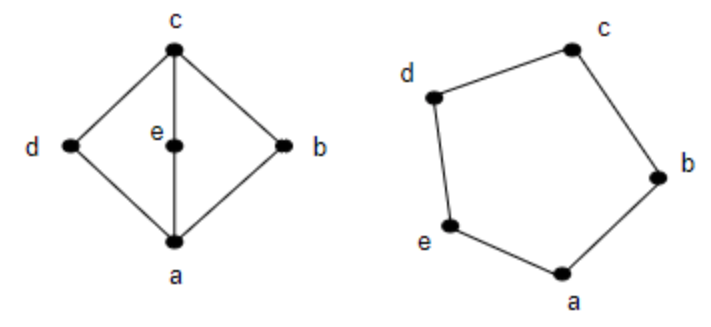
\includegraphics[scale=0.2]{img/Birkhoff.png}

    Osservazioni:

    Un reticolo totalmente ordinato è sempre distributivo.

    Tutti i reticoli di ordine $n<5$ sono distributivi.
}
\section{Principio di Induzione}
\bottom{
    Sia $x\subseteq\mathbb N\smallsetminus\{0\}$ Definiamo:
    $$\mathbb N_{min(x)}=\{n\in\mathbb N\ |\ min(x)\leq n\}$$
    Ovvero l'insieme che contiene tutti i numeri naturali $\geq$ del minimo dell'insieme $x$.
}
\subsection{Prima Forma del Principio di Induzione}
\bottom{
    $$\forall x \in P(\mathbb N) - \{\emptyset\}$$
    $$\forall n \in \mathbb N$$
    $$((n \in x \implies n + 1 \in x) \implies (x = \mathbb N_{min(x)}))$$
}
\bottomp{
    Sia $m=min(x)$. Ipotizziamo per assurdo che $x\not=\mathbb N_m$.
    Questo implica che $$y = \mathbb N_m - x \neq \emptyset$$
    Poniamo $min(y)=n$, che esiste sicuramente perchè $y\subseteq\mathbb N$.
    $$m<n$$
    poiché
    $$x \cap y = \emptyset \land n \in \mathbb N_m$$
    Quindi $$m \leq n-1 < n \implies (n - 1) \in x$$
    Per ipotesi, allora
    $$(n - 1) + 1 \in x \implies n \in x$$
    che è assurdo.
}

\subsection{Seconda Forma del Principio di Induzione}
\bottom{
    $$\forall x \in P(\mathbb N) - \{\emptyset\}$$
    $$\forall n \in \mathbb N$$
    $$\forall k \in \mathbb N$$
    $$((min(x) \leq k < n \implies k \in x) \implies n \in x) \implies (x = \mathbb N_{min(x)})$$
}
\bottomp{
    Sia $m=min(x)$ e supponiamo per assurdo che $x\not=\mathbb N_m$. Questo implica che 
    $$x\subset \mathbb N_m \implies y=\mathbb N_m -x\not=\emptyset$$
    Allora si ha che $$\forall k\in\mathbb N\ (m\le k<min(y) \implies k\in x)$$
    e quindi per ipotesi $min(y)\in x$, che è assurdo.
}
\section{Calcolo Combinatorio}
\subsection{Equipotenza}
\bottom{
    Due insiemi \(x, y\) si dicono equipotenti se esiste una funzione \(f: x \to y\) biettiva.
}

\subsection{Insieme Infinito}
\bottom{
    Un insieme \(x\) si dice infinito se esiste una bisezione \(f: x \to t \subset x\)
    ovvero se esiste una biezione tra se stesso ed una sua parte propria.
}

\subsection{Insieme Finito}
\bottom{
    Si dimostra che \(\forall n \in \mathbb N\ (\{1, ..., n\} \text{ non infinito})\).
    Un insieme \(x\) equipotente ad un insieme \(\{1, ..., n\} \subset \mathbb N\) si dice finito.
}

\subsection{Cardinalità di un Insieme Finito}
\bottom{
    Sia \(x\) finito. Allora \(\exists n \in \mathbb N\ (x \text{ equipotente a } \{1, 2, ..., n\} \subset \mathbb N)\). Diciamo che \(n\) è l'ordine o cardinalità di \(x\) e lo notiamo \(|x|=n\).
}

\subsection{Cardinalità dell'Insieme delle Parti di un Insieme Finito}
\bottom{
    \(s\) insieme finito \(\implies |P(s)| = 2^{|s|}\)
}
\bottomp{
    Dimostriamo per Induzione di Prima Forma su \(n\) cardinalità dell'insieme \(s\).
    Caso base: $$n = |s| = 0 \implies s = \emptyset \implies P(s) = \{\emptyset\} \implies |P(s)| = 1 = 2^0 $$
    Dunque la tesi è valida nel caso base. Ipotizziamo che sia valida per \(n \in \mathbb N\) e dimostriamo che vale per \(n + 1\).

    $$|s| = n + 1 \implies s \neq \emptyset \land \exists f: s \to \{1, 2, ..., n, n + 1\} \text{ biettiva}$$
    Consideriamo un qualunque \(x \in s\) e poniamo \(t = s - \{x\}\). Si ha che $$1 \leq f(x) = m \leq n+1$$ Si osserva che la funzione ristretta e ridotta $$f_{|t}: t \to Im_{f_{|t}} = \{1, 2, ..., m - 1, m + 1, ..., n, n +1\} \text{ è biettiva}$$ Si può definire una biezione fra \(Im_{f_{|t}}\) e \(\{1, ..., n\}\) e quindi \(|t| = n\).

    Per ipotesi induttiva, dunque \(|P(t)| = 2^n\).

    Ogni sottoinsieme di \(s\) può contenere o non contenere \(x\). I sottoinsiemi che non contengono \(x\) sono esattamente i sottoinsiemi di \(s - \{x\}\), che è un insieme con un elemento in meno ad \(s\), cioè \(|s -x| = n\). Per ipotesi induttiva quindi ne esistono \(2^n\). 
    Ogni sottoinsieme di \(s\) che contiene \(x\) può essere espresso come \(p \cup \{x\}, p \in s-\{x\}\). Dato che esistono \(2^n\) insiemi \(p\), allora esisteranno \(2^n\) insiemi che contengono \(x\).
    Dunque:
    $$|P(s)| = 2^n \cdot 2^n = 2^n+1$$

    Che è la tesi induttiva. Pertanto essa vale \(\forall n \in \mathbb N\).
}

\subsection{Fattoriale}
\bottom{
    Defiamo $$0! = 1$$
    Poi, ricorsivamente, definiamo:
    $$n! = n\cdot (n - 1)! $$
}

\subsection{Numero di Applicazioni fra Due Insiemi Finiti}
\bottom{
    Siano \(a, b\) due insiemi. Allora esistono \(|b|^{|a|}\) applicazioni \(f: a \to b\).
}
\bottomp{
    Poniamo \(|a| = m, |b| = n\). Usiamo la Prima Forma del Principio di Induzione su \(m\).

    Consideriamo \(m = 0\) come caso base, cioè \(a = \emptyset\).
    Dato che \(\emptyset \times b = \emptyset\) e il vuoto ha un solo sottonsieme \(\emptyset \subseteq \emptyset \times b\) che può fare da grafico per un'applicazione, esiste una sola possibile applicazione \((\emptyset \times b, \emptyset)\) fra i due insiemi. Dato che \(n^0 = 1\), la tesi è valida nel caso base.

    Ipotizzando dunque che la tesi sia valida per \(m > 0\), dimostriamo che vale per \(m+1\).
    Sia \(x \in a\) e \(t = a - \{x\}\). Per ipotesi induttiva, esistono \(n^m\) applicazioni da \(t \to b\).
    Ognuna di queste funzioni potrebbe essere prolungata, associando \(x\) ad uno qualsiasi degli \(n\) elementi di \(b\). Pertanto per ogni funzione esistono \(m\) possibili prolungamenti, e quindi il numero totale di applicazioni è \(n^m \cdot n = n^{m+1}\) che è la tesi.
}

\subsection{Condizione di Esistenza di Applicazioni Iniettive fra due Insiemi Finiti}
\bottom{
    $$MAP_{IN}(a, b) \neq \emptyset \iff |a| \leq |b|$$
    Esistono applicazioni iniettive fra due insiemi \(a\) e \(b\) se e solo se la cardinalità di \(a\) è minore o uguale di quella di \(b\).
}
\bottomp{
    Poniamo \(m = |a|, n = |b|\).

    \(\Rightarrow\)) Esiste una biezione \(I_m \to a\), almeno una funzione \(f \in MAP_{IN}(a, b)\), e una biezione \(b \to I_n\). Pertanto, la loro composizione è una funzione iniettiva da \(I_m \to I_n\). Pertanto, \(m \leq n\) in quanto per ognuno degli \(m\)-esimi elementi deve esistere almeno un elemento distinto in \(I_n\). 

    \(\Leftarrow)\)Se \(m \leq n\), allora \(\{1, ..., m\} \subseteq \{1, ..., n\}\) ed esiste quindi la funzione immersione fra i due, che è una funzione iniettiva. Esiste dunque una biezione da \(a \to \{1, ..., m\}\), una funzione iniettiva (l'immersione) da \(\{1, ..., m\} \to \{1, ...,n\}\) ed una biezione da \(\{1, ..., n\} \to b\) e dunque esiste una funzione iniettiva \(a \to b\).
}

\subsection{Numero di Applicazioni Iniettive fra due Insiemi Finiti}
\bottom{
    $$MAP_{IN}(a, b) \neq \emptyset \implies |MAP_{IN}(a,b)| = \frac{|b|!}{(|b|-|a|)!}$$
    Cioè, se esistono applicazioni iniettive fra due insiemi finiti, quello è il loro numero.
}
\bottomp{
    Poniamo \(|a| = m, |b| = n\), \(m \leq n\) altrimenti non esisterebbero applicazioni iniettive. Dimostriamo per Induzione di Prima Forma su \(m\).

    Caso base: \(m = 0\). Quindi \(a = \emptyset\). Esiste una sola funzione fra il vuoto e \(b\), ed essa è iniettiva in quanto verifica vacuamente l'implicazione nella definizione di iniettività. Dato che \(\frac{n!}{(n - 0)!} = 1\) la tesi è valida.

    Ipotizziamo dunque che la tesi sia valida anche per \(\forall (m - 1) > 0\), e dimostriamo che è valida in \(m\).
    Siano \(x \in a, t = a - \{x\}\). Dunque \(|t| = m - 1\) ed esistono \(\frac{n!}{(n - (m-1))!}\) applicazioni iniettive \(t \to b\) per ipotesi induttiva. Ognuna di queste può essere prolungata ad \(a\) associando \(x\) ad uno qualsiasi degli \(n - (m - 1)\) elementi rimasti in \(b\) (dato che dobbiamo scegliere, per lasciare la funzione iniettiva, un'immagine distinta).

    Da ciò segue che esistono \(\frac{n!}{(n - (m-1))!} \cdot (n - (m - 1))\) funzioni iniettive, e sviluppando:

    $$\frac{n!}{(n - (m-1))!} \cdot (n - (m - 1)) = \frac{n!}{\cancel{(n - m +1)!}} \cdot \cancel{(n - m + 1)} = \frac{n!}{(n - m)!}$$
}

\subsection{Condizione di Esistenza di Applicazioni Suriettive fra due insiemi Finiti}
\bottom{
    $$MAP_{SUR}(a, b) \neq \emptyset \iff a = b = \emptyset \lor 0 < |b| \leq |a|$$
    Esistono applicazioni suriettive fra due insiemi \(a\) e \(b\) se e solo se sono entrambi vuoti o se sono entrambi non vuoti e la cardinalità di \(a\) è maggiore o uguale di quella di \(b\).
}
\bottomp{
    Sia \(|a| = m, |b| = n\). 

    \(\Rightarrow)\) Sia \(f: a \to b\) suriettiva. Allora esiste una biezione fra \(a \to \{1, ..., m\}\) , una funzione suriettiva \(a \to b\), ed una biezione \(b \to \{1, ..., n\}\). Pertanto esiste una funzione suriettiva \(\{1, ..., m\} \to \{1, ..., n\}\). Allora per ogni elemento del secondo insieme esiste un elemento distinto (dalla definizione di applicazione) del primo insieme, pertanto \(n \leq m\).

    \(\Leftarrow)\) Se sono entrambi non vuoti e \(n \leq m \implies I_n\), allora è banale costruire una funzione suriettiva dato che per ogni possibile elemento di \(b\) si può scegliere un elemento distinto di \(a\).

    Dimostrazione nel caso particolare in cui sono vuoti:
    Se \(b = \emptyset\), allora \(a\) dev'essere anch'esso il vuoto altrimenti non si può avere funzione ben formata fra i due, dato che per ogni elemento di \(a\) dev'esistere un elemento di \(b\) sua immagine. Se \(a = \emptyset\) e \(b\) è non vuoto, allora la funzione non può essere suriettiva. Se \(a = b = \emptyset\) allora la suriettività $$\forall y\ (y \in b \implies \exists x \in a\ (y = f(x))$$ è provata vacuamente dato che \(y \in b\) è sempre falso.
}

\subsection{Condizione di Esistenza di Applicazioni Biettive fra due Insiemi Finiti}
\bottom{
    Dalla condizione di esistenza delle funzioni iniettive e da quella per le funzioni suriettive deriva che, dati insiemi finiti \(a, b\):
    $$MAP_{BI}(a, b) \neq \emptyset \iff |a| = |b|$$
}

\subsection{Cardinalità dell'Insieme Simmetrico di un Insieme Finito}
\bottom{
    $$|SYM(a)| = |a|!$$}{L'insieme simmetrico è l'insieme delle applicazioni biettive \(a \to a\). Quindi, dominio e codominio hanno stessa cardinalità e dunque ogni funzione iniettiva è biettiva. Pertanto, possiamo usare la formula per il calcolo del numero delle funzioni iniettive per calcolare le biettive:

    $$|SYM(a)| = \frac{|a|!}{(|a| - |a|)!} = \frac{|a|!}{0!} = \frac{|a|!}{1} = |a|!$$
}

\subsection{Relazione fra Iniettività e Suriettività di Applicazioni fra Insiemi Finiti di Uguale Cardinalità}
\bottom{
    Siano \(a, b\) insiemi e \(f: a \to b\) una funzione. Allora:

    \(|a| = |b| \implies (f \text{ iniettiva} \iff f \text{ suriettiva} \iff f \text{ biettiva})\)}{Poniamo \(|a| = |b| = m\).
    Se \(f: a \to b\) è una funzione iniettiva, la sua immagine ha \(|m|\) elementi. Ma $$Imf \subseteq b \land |Imf| = |b| = m$$ dunque \(Imf = b\) e la funzione è anche suriettiva.
    Se \(f: a \to b\) è una funzione suriettiva, allora esiste sezione \(g: b \to a\) tale che \(f \circ g = Id_b\). Ma dato che \(Id_b\) è biettiva, e dunque iniettiva, allora \(g\) è iniettiva. Allora, per come mostrato sopra, essa è anche suriettiva, e dunque è biettiva, e quindi \(f\) è la sua inversa ed è biettiva a sua volta.
}

\subsection{Cancellabilità implica Invertibilità in un Monoide Commutativo Finito}
\bottom{
    Sia \((s, \cdot)\) un monoide commutativo finito e sia \(x \in s\). Allora \(x\) è invertibile se e solo se è cancellabile.
}
\bottomp{
    In generale, l'invertibilità implica la cancellabilità, indipendentemente che l'insieme sia finito o no.
    Se \(x\) è cancellabile, allora \(\sigma_x\) e \(\delta_x\) sono iniettive, ma essendo \(s\) finito, allora esse sono anche biettive (per il teorema precedente), e quindi:
    $$\exists y \in s\ (\sigma_x(y) = xy = 1_s)$$ e quindi \(y\) è inverso a destra.
    $$\exists z \in s\ (\delta_x(z) = zx = 1_s)$$ e quindi \(z\) è inverso a sinistra.
    Allora \(y = z\) e \(x\) è invertibile.
}

\subsection{Anelli Unitari Integri Finiti sono Corpi}
\bottom{
    Corollario di "Invertibilità e Cancellabilità in un Monoide Commutativo Finito".

    Tutti gli anelli unitari integri finiti sono corpi.
}
\bottomp{
    Un anello unitario integro è un corpo se e solo se ogni elemento è invertibile rispetto al prodotto. Essendo integro, non esistono divisori dello zero. Pertanto ogni elemento distinto dallo zero è cancellabile. Essendo l'anello per ipotesi finito, allora, per il teorema di cui questo è corollario, ogni elemento distinto dallo zero è inverbile, e dunque l'anello è un corpo.
}

\subsection{Domini di Integrità Finiti sono Campi}
\bottom{
    Corollario di "Invertibilità e Cancellabilità in un Monoide Commutativo Finito"
}
\bottomp{
    Un dominio di integrità finito è un anello unitario integro finito, pertanto, per "Anelli Unitari Integri Finiti sono Corpi", esso è un corpo. Ma un dominio di integrità è commutativo, ed un corpo commutativo è proprio un campo.
}

\subsection{Funzione Caratteristica}
\bottom{
    Sia \(s\) un insieme e \(t \subseteq s\). Allora l'applicazione:

    \(\chi_{t, s}: x \in s \mapsto \begin{cases}0 \text{ se } x \notin t\\ 1 \text{ se } x \in t\end{cases}\)

    Si dice applicazione caratteristica di \(t\) in \(s\).
}

\subsection{Ogni sottoinsieme è dotato di funzione caratteristica}
\bottom{
    \(\varphi: t \in P(s) \mapsto \chi_{t, s} \in \{0, 1\}^s\) è biettiva.
    \(\varphi: t \in P(s) \mapsto \chi_{t, s} \in \{0, 1\}^s\) è biettiva. Cioè, esiste una corrispondenza biunivoca fra le parti di un insieme e le funzioni \(\{0, 1\}^s\). Cioè, ogni parte ha una funzione caratteristica ed ogni funzione a due immagini è funzione caratteristica di un qualche sottoinsieme di \(s\).
}
\bottomp{
    Suriettività) Sia \(f \in \{0, 1\}^s\). Poniamo $$t = \overleftarrow{f}(\{1\}) = \{x \in s \mid f(x) = 1\}$$
    Se \(x \in t \implies \chi_{t, s} = 1 = f(x)\) per costruzione di \(t\).
    Se \(x \notin t \implies \chi_{t, s} = 0 = f(x)\) per costruzione di \(t\).
    Quindi \(f = \chi_{t,s}\) e \(\varphi\) è suriettiva.

    Iniettività) Sia $$t \subseteq s \land v \subseteq s \land t \neq v$$ Senza ledere la generalità prendo \(x \in t - v\). Allora \(\chi_{t,s}(x) = 1\) e \(\chi_{v,s} = 0\) quindi le funzioni sono distinte e \(\varphi\) è iniettiva.
}

\subsection{Coefficiente Binomiale}
\bottom{
    \(\forall n, k \in \mathbb N\) definiamo:

    $${n \choose k} = |P_k(I_n)|$$

    Se \(n < k\), allora \({n \choose k} = 0\)
}

\subsection{Sommatoria di Coefficienti Binomiali}
\bottom
{
    $$\forall n \in \mathbb N\ (\sum_{k = 0}^{n} {n \choose k} = 2^n$$
}    
\bottomp{
    Si osserva che $$P(I_n) = P_0(I_n) \cup P_1(I_n) \cup ... \cup P_n(I_n)$$

    Che sono tutti insiemi disgiunti, pertanto si ha che:

    $$|P(I_n)| = |P_0(I_n)| \cup |P_1(I_n)| \cup ... \cup |P_n(I_n)| = \sum_{k = 0}^{n} {n \choose k} = 2^n $$
}

\subsection{Equivalenza di Coefficienti Binomiali}
\bottom{
    $$\forall n, k \in \mathbb N\ (k \leq n \implies {n \choose k} = {n \choose n - k})$$
}
\bottomp{
    Sia $$f: x \in P(I_n) \mapsto I_n - x \in P(I_n)$$ \(f\) è biettiva perché la funzione differenza di insiemi è biettiva. Inoltre, ovviamente, se $$|I_n| = n, |x| = k \implies |I_n - x| = n - k$$ e dunque:
    $$\overrightarrow f(P_k(I_n)) = P_{n - k}(I_n)$$

    Quindi la funzione:
    $$f_{|P_k(I_n)}: x \in P_k(I_n) \mapsto I_n - x \in P_{n - k}(I_n) = Imf_{|P_k(I_n)}$$
    E' ancora una biezione. I due insiemi sono equipotenti e dunque:

    $${n \choose k} = |P_k(I_n)| = |P_{n - k}(I_n)| = {n \choose n - k}$$

    Che è la tesi.
}

\subsection{Formula Ricorsiva per i Coefficienti Binomiali}
\bottom{
    $$\forall n, k \in \mathbb N\ (k \leq n \implies {n+1 \choose k+1} = {n \choose k} + {n \choose k+1})$$
}
\bottomp{
    Sia \(I_{n+1}\). Allora definisco:
    $$
    a = \{x \in P_{k+1}(I_{n+1}) \mid 1 \in x\}
    $$
    $$
    b = \{y \in P_{k+1}(I_{n+1}) \mid 1 \notin y\}
    $$

    Se rimuovessimo \(1\) da ogni \(x \in a\), questo diminuirebbe la loro cardinalità di uno, rendendola \(k\). Non contenendo \(1\), sarebbero poi anche sottoinsiemi di cardinalità \(k\) dell'insieme \(I_{n+1} - \{1\}\), e sarebbero quindi \({n \choose k}\) in numero.

    Similarmente, gli insiemi di \(b\), non contenendo \(1\), sono gli insiemi di cardinalità \(k+1\) dell'insieme \(I_{n+1} - \{1\}\) e quindi sono \({n \choose k + 1}\) in numero.

    \(\{a, b\}\) è una partizione di \(P_{k+1}(I_{n+1})\), e quindi, per il Principio di Inclusione-Esclusione:
    $${n+1 \choose k+1} = |P_{k+1}(I_{n+1})| = |a| + |b| = {n \choose k}+ {n \choose k+1}$$
}

\subsection{Triangolo di Tartaglia}
\bottom{
    Triangolo dei Coefficienti Binomiali, che permette di calcolare graficamente il valore di un qualsiasi coefficiente binomiale grazie alla Formula Ricorsiva dei Coefficienti Binomiali.
    \\\\
    \includegraphics*[scale=.25]{img/tartaglia.png}
}

\subsection{Formula Matematica per il Calcolo dei Coefficienti Binomiali}
\bottom{
    $$\forall n, k \in \mathbb N\ (k \leq n \implies {n \choose k} = \frac{n!}{(n-k)!k!})$$
}
\bottomp{
    Dimostriamo per induzione di seconda forma. Prima di tutto, dobbiamo organizzare i coefficienti binomiali in "linea", in modo che ad ogni coefficiente binomiale possa essere associato un intero. Utilizziamo quindi un ordine lessicografico e diciamo che:

    $$\forall x, y, z, w \in \{0, ..., n\}\ ((x, y) < (z, w) \iff (x < z) \land (y < w))$$

    Si osserva dunque che le coppie associate ai coefficienti binomiali sono così ordinate:

    \((0, 0) < (1, 0) < (1, 1) < (2, 0) < (2,1) < (2, 2) < (3, 0) < (3, 1) < (3, 2) < (3, 3) < (4, 0) < \dots\)

    Ora che le coppie sono così messe in ordine, possiamo dire quale sia la zeresima, prima, seconda, n-esima coppia, etc.

    Usiamo come caso base l'indice \(m = 0\), cioè la zeresima coppia, \({0 \choose 0}\). Esiste un solo insieme di cardinalità zero sottoinsieme del vuoto, il vuoto stesso, quindi $$1 = \frac{0!}{(0 - 0)!0!}$$ e la tesi vale nel caso base.

    Estendiamo la tesi ad ogni \(0 \leq i < m\) per ipotesi induttiva, e dimostriamo che essa vale in \(m\).
    Ipotizziamo che la coppia di indice \(m\) sia \({n \choose k}\). Per la Formula Ricorsiva per i Coefficienti Binomiali, allora:

    $${n \choose k} = {n - 1 \choose k - 1} + {n-1 \choose k}$$

    Ma per l'ordine lessicografico, questi sono minori di \({n \choose k}\), quindi vale per essi la tesi induttiva, e quindi:

    $${n - 1 \choose k - 1} + {n-1 \choose k} = \frac{(n-1)!}{(n-1-(k-1))!(k-1)!} + \frac{(n-1)!}{(n-1-k)!k!}=$$
    $$ =
    \frac{(n-1)!}{(n-k)!(k-1)!} + \frac{(n-1)!}{(n-k-1)!k!} =
    $$
    $$=\frac{(n-1)!k}{(n-k)!k!} + \frac{(n-1)!(n-k)}{(n-k)!k!}=  \frac{(n-1)!(k + n - k)}{(n-k)!k!}=$$
    $$ = \frac{(n-1)!n}{(n-k)!k!} = \frac{n!}{(n-k)!k!}
    $$
}
\section{Strutture Booleane}
\subsection{Reticolo Booleano}
\bottom{
    Un reticolo si dice booleano se è distributivo e complementato
}

\subsection{Algebra di Boole}
\bottom{
    Una struttura della forma $(s,\land_\rho,\lor_\rho,')$ si dice Algebra di Boole se gode delle seguenti proprietà:
    \begin{enumerate}
        \item $\land_\rho,\lor_\rho$ sono commutative
        \item Esse sono anche associative
        \item Valgono le leggi di assorbimento
        \item Vale la distributività
        \item $\land_\rho,\lor_\rho$ hanno elementi neutri, che notiamo rispettivamente 0 e 1
        \item $'$ è un operazione unaria interna (l'operazione complementazione) tale che:
        $$\forall x \in s\ (x \vee_\rho x' = 1) \land (x \wedge_\rho x' = 0)$$
    \end{enumerate}
}

\subsection{Anello Booleano}
\bottom{
    Un anello unitario $(a,+,\cdot)$ si dice booleano $\iff$
    $$\forall x \in a\ (x^2 = x\cdot x=x)$$
    Ovvero ogni elemento è idempotente.
}

\subsection{In un Anello Booleano ogni elemento è il Proprio Opposto}
\bottom{
    $$(a, +, \cdot) \text{ anello booleano} \implies \forall x \in a\ (x = -x)$$
}
\bottomp{
    \begin{align*}
        x + x &= (x + x)^2 &\text{ per proprietà degli anelli booleani}\\
        &= x^2 + 2x^2 + x^2 &\text{ per distributività dell'anello}\\
        &= x + 2x + x
    \end{align*}
    Quindi $$x + x = x + 2x + x \implies 2x = 0 \implies x + x = 0 \implies x = -x$$
}

\subsection{Anelli Booleani sono Commutativi}
\bottom{
    Sia $(a,+,\cdot)$ un anello booleano. Allora $(\forall x, y \in a)(xy = yx)$
}
\bottomp{
    Siano $x,y\in a$. Allora:
    \begin{align*}
        x + y &= (x + y)^2 &\text{ prop. dell'anello booleano}\\
        &= x^2 + xy + yx + y^2 &\text{ prop. distributiva}\\
        &= x + xy + yx + y &\text{ prop. dell'anello booleano}\\
        &\implies xy + yx = 0 \implies xy = -yx
    \end{align*}
    In quanto ogni elemento dell'anello è il proprio opposto $-yx=yx$ quindi abbiamo la tesi.
}

\subsection{Per ogni Anello Booleano esiste un corrispondente Reticolo Booleano}
\bottom{
    Dato un anello booleano $(a,+,\cdot)$ definiamo 
    $$\rho:\forall x,y\in a\ (x\rho y\iff xy=x)$$
    Allora vogliamo dimostrare che $(s,\rho)$ è un reticolo.
}
\bottomp{
    Iniziamo col dimostrare che $\rho\in OL(a)$
    $$\forall x \in a\ (x \cdot x = x) \implies \forall x\ (x \rho x)$$
    per la proprietà principale dell'anello booleano e quindi la relazione è riflessiva.
    $$\forall x, y \in a\ (x \rho y \land y \rho x \implies xy = x \land yx = y \implies x = y)$$
    per la commutatività dell'anello booleano e quindi la relazione è asimmetrica.
    $$\forall x, y, z \in a$$
    $$x \rho y \land y \rho x \implies xy = x \land yz = y \implies$$
    $$ x = xy = x(yz) = (xy)z = xz \implies x \rho z$$
    la relazione è dunque transitiva.
}
\bottom{
    Dimostrazione $\land$ e $\lor$

    Verifichiamo per ogni coppia che INF e SUP sono così definite:
    $$\forall x, y \in a\ (x \wedge_\rho y = xy)$$
    $$\forall x, y \in a\ (x \vee_\rho y = x+ y + xy)$$
}
\bottomp{
    Dimostriamo che $x\lor_\rho y$ è maggiorante.
    $$x \cdot (x \vee_\rho y) = x(x + y + xy) = x^2 + xy + x^2y$$
    Per le proprietà dell'anello booleano
    $$x^2 = x \text{ e } xy + xy = 0$$
    Pertanto $x \cdot (x \vee_\rho y) = x \implies x \rho (x \vee_\rho y)$ perchè $x\rho y\iff xy=x$.

    Lo stesso procedimento si può effettuare per $y$.

    Pertanto $x\vee_\rho y$ è maggiorante.
}
\bottomp{
    Dimostriamo che $x \vee_\rho y$ è estremo superiore, cioè minimo dei maggioranti.
    Sia $z\in a$ maggiorante di $\{x,y\}$. Allora
    \begin{align*}
        &x\rho z\ \land\ y \rho z\\
        &\implies (xz =x)\ \land\ (yz = y)\\
    &\implies (x + y + xy)z = xz + yz + xyz = x + y + xy\\
    &\implies (x + y + xy)\rho z\\
    &\implies (x \vee_\rho y)\rho z
    \end{align*}
    quindi $(x\vee_\rho y)$ è sup.
}
\bottomp{
    Dimostriamo che il Reticolo è limitato, distributivo e complementato.

    Limitato)
    $$\forall x \in a\ (0x = 0 \implies 0\rho x)$$
    cioè 0 è il minimo
    $$\forall x \in a\ (1x = x \implies x \rho 1)$$
    cioè 1 è il massimo, quindi il reticolo è limitato.

    Distributivo)
    $$x \wedge (y \vee z) = x \wedge (y + z + yz) = x(y + z + yz) = xy + xz + xyz$$
    pertanto il reticolo è distributivo.

    Complementato) Sia $x\in a.$ Allora
    $$x \wedge (1+x) = x(1+x) = x + x^2 = x + x = 0$$
    $$x \vee (1+x) = x + (1+x) + x(1+x) = x + 1 + x + x + x^2 = 1$$
    questo perchè ogni elemento è anche il suo opposto.
}

\subsection{Per ogni Reticolo Booleano esiste un corrispondente Anello Booleano}
\bottom{
    Sia $(s,\rho)$ un reticolo booleano con almeno due elementi e definiamo:
    $$x + y = (x \wedge_\rho y') \vee_\rho (x' \wedge_\rho y)$$
    $$x \cdot y = (x \wedge_\rho y)$$
    Dimostriamo che $(s,+,\cdot)$ è un anello booleano
}
\bottomp{
    Dimostrare che è un anello booleano vuol dire dimostrare che è un anello unitario dove $\forall x \in s\ (x^2 = x)$.

    Associatività:
    $$x(yz) = x \wedge (y \wedge y) = (x \wedge y) \wedge y = (xy)z$$
    Si dimostra analogamente, ma con una LUNGA serie di calcoli, che vale lo stesso per $x+y$.

    Commutatività di $+$:
    $$x + y = (x \wedge y') \vee (x' \wedge y) = (y' \wedge x) \vee (y \wedge x') = (y \wedge x') \vee (y' \wedge x) = y+x $$
    Definiamo $$m = min_{(s, \rho)}(s), M = max_{(s, \rho)}(s)$$ Allora
    $$x + m = (x \wedge m') \vee (x' \wedge m) = (x \wedge M) \vee (x' \wedge m) = x \vee m = x$$
    $$x \cdot M = x \wedge M = x$$
    Dunque $m=0_s$ e $M=1_s$

    Si dimostra tramite calcolo che vale al distributività di $\cdot$ su $+$.

    Infine:
    $$x^2 = x \cdot x = x \wedge x = x$$
    ed abbiamo la tesi.
}

\subsection{Equivalenza di Strutture Booleane}
\bottom{
    Si dimostra quindi che
    \begin{center}
        Algebre di Boole \(\simeq\) Reticoli di Boole \(\simeq\) Anelli Booleani
    \end{center}
    In quanto esiste una corrispondenza biunivoca fra le tre strutture.
}

\subsection{L'insieme delle Parti è un Anello Booleano}
\bottomp{
    Dato che $(P(s),\subseteq)$ è un reticolo booleano, allora $(P(s), \cap, \cup, ')$ è un'algebra di boole, dove$$\forall x \in P(s)\ (x' = s - x)$$ per la corrispondenza biunivoca fra reticoli booleani ed algebre di boole. Allora
    $$\forall x, y \in P(s)$$
    $$x \cdot y = x \cap y$$
    $$x + y = (x \cap (s - y)) \cup (y \cap (s -x)) = (x - y) \cup (y - x) = x \triangle y$$
    E dunque $(P(s), \triangle, \cap)$ è un anello booleano.
}

\subsection{Teorema di Stone}
\bottom{
    Sia $a\not=\emptyset$ e $(a,+,\cdot)$ un anello booleano. Allora
    $$\exists s \neq \emptyset$$
    $$(a, +, \cdot) \stackrel{\text{isomorfo}}{\simeq} (P(s), \triangle, \cap)$$
    Se $a$ è finito, posso scegliere anche $s$ finito.
}

\subsection{Corollari del Teorema di Stone}
\bottom{
    \begin{enumerate}
        \item Il Teorema di Stone si applica anche fra reticoli booleani e ${{(P(s), \subseteq)}}$.
        \item Se $(a,+,\cdot)$ è un anello booleano e $|a|=m\in\mathbb N_2$, allora 
        $$(\exists n \in \mathbb N - \{0\})(m = 2^n)$$
        \item Se $(a,\rho)$ è un reticolo booleano e $|a|=m\in\mathbb N_1$, allora $$(\exists n \in \mathbb N - \{0\})(m = 2^n)$$
        cioè la cardinalità dell'insieme sostegno di un anello booleano è sempre una potenza di due.
        \item Due anelli booleani finiti sono isomorfi $\iff$ hanno la stessa cardinalità.
    \end{enumerate}
}
\section{Stringhe}
\subsection{Insieme delle Stringhe}
\bottom{
    Scriviamo: \(\mathbb Z_2 = \mathbb Z / \equiv_2 = \{[0]_2, [1]_2\}\).
    Allora, dato \(n \in \mathbb N\), definiamo \(a = \mathbb Z_2 \times ... \times \mathbb Z_2 \text{ (} n \text{ volte)}\) l'insieme delle stringhe di 0 ed 1 di lunghezza \(n\).
}

\subsection{Somma e Prodotto Puntuali di Stringhe}
\bottom{
    Sia \(a = \mathbb Z_2 \times ... \times \mathbb Z_2\), \(n \in \mathbb N\) volte. Allora, presi \(x, y \in a\) tali che \(x = (x_1, ..., x_n), y = (y_1, ..., y_n), x_i, y_i \in \{0, 1\} \forall i \in I_n\), allora definiamo la somma puntuale:
    $$x + y = ([x_1 + y_1], [x_2 + y_2], ..., [x_n + y_n])$$
    Analogamente, definiamo il prodotto puntuale:
    $$x \cdot y = ([x_1 \cdot y_1], ..., [x_n \cdot y_n])$$
}

\subsection{Stringhe e Funzioni Caratteristiche}
\bottom{
    Dato un insieme \(s: |s| = n > 0\) e \(t \subseteq s\), allora la funzione caratteristica \(\chi_{t, s}\) può essere vista analoga ad una stringa, dato che associa ad ogni elemento di \(t\) o 0 o 1.
}

\subsection{L'Anello delle Parti e l'Anello delle Stringhe sono Isomorfi}
\bottom{
    Sia \(n \in \mathbb N - \{0\}\) e \(s = \{1, 2, ..., n\}\). Allora la funzione $$\varphi: x \in P(s) \mapsto \chi_{t, s} \in \mathbb Z_2 \times ... \mathbb Z_2$$ (\(n\) volte) è un'isomorfismo fra $$(P(s), \triangle, \cap)$$ e $$(\mathbb Z_2 \times ... \times \mathbb Z_2 \text{ (n volte)}, +, \cdot)$$ (dove \(+, \cdot\) sono la somma e prodotto puntuali).
}
\include{Capitoli/Divisibilità}
\section{Polinomi}
\subsection{  Definizione di Successione di Elementi}
\bottom{
    Sia \((a, +, \cdot)\) un anello unitario commutativo. Allora una funzione del tipo \(n \in \mathbb N \mapsto x \in a\) si dice successione di elementi di \(a\).
}

\subsection{ Notazione di Successione di Elementi}
\bottom{
    Sia \((a, +, \cdot)\) un anello commutativo unitario. Sia \(f: n \in \mathbb N \mapsto x \in a\) una successione di elementi di \(a\). Allora:

    $$(a_n)_{n \in \mathbb N} := f$$
    $$a_n = f(n)$$
}

\subsection{ Polinomio}
\bottom{
    Sia \((a, +, \cdot)\) un anello commutativo unitario e sia \((a_n)_{n \in \mathbb N}\) una successione di elementi di \(a\). Allora:

    $$(a_n)_{n \in \mathbb N} \text{ poliniomio a coefficienti in } a \iff \exists k \in \mathbb N\ (\forall n \geq k\ (a_n = 0))$$ 
}

\subsection{ Coefficienti di un Polinomio}
\bottom{
    I termini di successione \(a_n\) di un polinomio \((a_n)_{n \in \mathbb N}\) si dicono coefficienti del polinomio.
}

\subsection{ Notazione di Insieme dei Polinomi}
\bottom{
    Sia \((A, +, \cdot)\) un anello commutativo unitario. Allora l'insieme dei polinomi a coefficienti in \(A\) si scrive \(A[x]\)
}

\subsection{ Polinomio Zero o Nullo}
\bottom{
    Sia \((a, +, \cdot)\) un anello commutativo unitario. Allora definiamo il polinimio nullo o polinomio zero:

    $$0 := (0_a)_{n \in \mathbb N}$$

    Dove $$(0_a)_{n \in \mathbb N} = (a_n)_{n \in \mathbb N}$$
    $$\forall n \in \mathbb N\ (a_n = 0_a)$$
}

\subsection{ Coefficiente Direttore di un Polinomio}
\bottom{
    Se \(f \in A[x] - \{0\}\), \(a_{gr(f)}\) si dice coefficiente direttore del polinomio e si indica \(cd(f)\)
}

\subsection{ Termine Noto di un Polinomio}
\bottom{
    Dato un polinomio \(f \in A[x]\), allora \(a_0\) si dice termine noto di \(f\).
}

\subsection{ Grado e Coefficiente Direttore del Polinomio Zero}
\bottom{
    Poniamo:

    $$cd(0) = 0$$
    $$gr(0) = -\infty$$

    Cioè il grado di \(0\) è l'ordinamento di \(\mathbb (N \cup \{-\infty\}, \leq)\)
}

\subsection{ Polinomio Monico}
\bottom{
    \(f \in A[x]\) si dice polinomio monico se \(cd(f) = a_{gr(f)} = 1_a\)
}

\subsection{ Somma e Prodotto di Polinomi}
\bottom{
    Siano \((a_n)_{n \in \mathbb N}, (b_n)_{n \in \mathbb N} \in A[x]\) due polinomi. Allora definiamo:

    $$(a_n + b_n)_{n \in \mathbb N} = (a_n)_{n \in \mathbb N} + (b_n)_{n \in \mathbb N}$$
    $$(\sum_{i+j=n}a_ib_j)_{n \in \mathbb N} = (a_n)_{n \in \mathbb N} \cdot (b_n)_{n \in \mathbb N}$$
}

\subsection{ Anello dei Polinomi}
\bottom{
    Avendo definito somma e prodotto per i polinomi, possiamo affermare che \((A[x], +, \cdot)\) è un anello commutativo unitario.
    \begin{itemize}
        \item Il neutro rispetto a \(\cdot\) è \((1, 0, 0, 0, ...)\)
        \item Il neutro rispetto a \(+\) è \((0, 0, 0, 0, ...)\)
    \end{itemize}
}

\subsection{ Polinomio Costante}
\bottom{
    Sia \((A, +, \cdot)\) un anello commutativo unitario e sia \(a \in A\). Allora il polinomio del tipo \((a, 0, 0, 0, 0, ...)\) si dice polinomio costante.
}

\subsection{ Notazione di Polinomio Costante}
\bottom{
    Facendo abuso di notazione, \(\forall a \in A\), definiamo \(a := (a, 0, 0, 0, 0, ...)\)
    Cioè indichiamo il polinomio costante con il suo unico coefficiente non nullo.
}

\subsection{ Monomorfismo dei Polinomi Costanti}
\bottom{
    Sia \((A, +, \cdot)\) un anello commutativo unitario. Si osserva allora che:

    $$\mu: a \in A \mapsto (a, 0, 0, 0, ...) \in A[x]$$

    è un monomorfismo di anelli fra \((A, +, \cdot)\) e \((A[x], +, \cdot)\).

    In particolare, $$a \stackrel {\text isomorfo}{ \simeq }Im(\mu)$$
}

\subsection{ Polinomio incognita}
\bottom{
    Definiamo il polinomio \(x := (0, 1_A, 0, 0, 0, 0, ...)\)
    Cioè il polinomio \(x \in A[x]\) tale che il suo unico coefficiente non nullo è l'unità dell'anello \((A, +, \cdot)\) nella seconda posizione.
}

\subsection{ Potenze del Polinomio incognita}
\bottom{
    Si può provare per induzione che:
    \begin{align*}
        x &= (0, 1, 0, 0, 0 ...)\\
        x^2 &= (0, 0, 1, 0, 0, ...)\\
        x^3 &= (0, 0, 0, 1, 0, ...)\\
        &\dots\\
        x^n &= (0, \dots, 0 \text{ (n volte)}, 1, 0, ...)
    \end{align*}
}

\subsection{ Monomio}
\bottom{
    Dato una anello \((A, +, \cdot)\), sia \(a \in A\), e sia \(x = (0, 1_A, 0, ...)\). Allora abbiamo che:
    $$ax^n = (a, 0, 0, 0,...) \cdot (0, \cdots, 0 \text{ (n volte)}, 1_a, 0, 0...)=$$
    $$ = (0, ..., 0 \text{ (n volte)}, a, 0, 0, ...)$$
    Il monomio $ax^n$ dunque non è nient'altro che il polinomio a coefficienti tutti nulli, eccetto quello in posizione n+1-esima, che ha valore a. (n+1 perchè la prima posizione è $x^0$).
}

\subsection{ Polinomio come Somma di Monomi}
\bottom{
    Sia \(f\) un polinomio tale che \(m \in \mathbb N \land gr(f) = m\) della forma $$f = (a_0, a_1, a_2, a_3, ..., a_m, 0, , ...)$$

    Allora è facile verificare che esso si può esprimere nella forma:
    $$f = a_0 + a_1x + a_2x^2 + a_3x^3 + ... + a_mx^m$$
}

\subsection{ Proprietà della Somma e Prodotto di Polinomi}
\bottom{
    Dalla distributività in \((A[x], +, \cdot)\) seguono le seguenti proprietà di somma e prodotto.
    Siano \(f, g \in A[x], m = gr(f), n = gr(g), M = max\{n, m\}\), allora:

    $$f + g = \sum_{i = 0}^M (a_i + b_i)x^i$$
    $$f \cdot g = \sum_{i=0}^{n+m}(\sum_{j=0}^i a_j b_{i - j})x^i$$
}

\subsection{ Proprietà del Grado della Somma di Polinomi}
\bottom{
    Siano \(f, g \in A[x] - \{0\}\). Allora:

    $$[gr(f) = gr(g)] \land [cd(f) = -cd(g)] \implies gr(f + g) < [gr(f) = gr(g)]$$
    $$[gr(f) \neq gr(g)] \lor [cd(f) \neq cd(g)] \implies gr(f + g) = max\{gr(f), gr(g)\}$$
}

\subsection{ Proprietà del Grado di Prodotto di Polinomi}
\bottom{
    Siano \(f, g \in A[x] - \{0\}\). Allora:

    $$cd(f) \cdot cd(g) = 0 \implies gr(f \cdot g) < gr(f) + gr(g)$$
    $$cd(f) \cdot cd(g)\neq 0 \implies gr(f \cdot g) = gr(f) + gr(g) \land cd(f \cdot g)=$$
    $$ = cd(f) \cdot cd(g) \text{ [FORMULA DI ADDIZIONE DEI GRADI]}$$

    Se $$f = 0, gr(f \cdot g) = gr(0) = -\infty = -\infty + gr(g)$$ e $$cd(f \cdot g) = 0 = cd(f) \cdot cd(g)$$ si osserva che la Formula di Addizione dei Gradi vale anche con il polinomio zero.
}

\subsection{ Coefficiente Direttore Cancellabile implica Polinomio Cancellabile}
\bottom{
    Sia \(f \in A[x] - \{0\}\). Se \(cd(f)\) è cancellabile, allora anche \(f\) lo è. In particolare, per \(f\) vale la Formula di Addizione dei Gradi.}{\(cd(f)\) cancellabile vuol dire che esso non è divisore dello zero. Per la Formula di Addizione dei Gradi segue che:
    $$\forall g \in A[x]$$
    $$g \neq 0 \implies gr(f \cdot g) = gr(f) + gr(g) \neq -\infty \implies f \cdot g \neq 0 \implies f$$ non è divisore dello zero, cioè \(f\) è cancellabile.
}

\subsection{ Condizione Sufficiente e Necessaria per Dominio di Integrità dei Polinomi}
\bottom{
    \(A[x]\) è dominio di integrità \(\iff A\) è dominio di integrità.
}

\subsection{ Condizione di Non Invertibilità di un Polinomio}
\bottom{
    Sia \(f \in A[x]\). Se \(f\) è cancellabile e \(gr(f) > 0\), allora \(f\) non è invertibile.
}
\bottomp{
    Per assurdo, sia \(f\) invertibile e sia \(g = f^{-1}\). Allora per la Formula di Addizione dei Gradi,  $$gr(f) + gr(g) = gr(fg) = gr(1) = 0 \implies gr(f) = 0$$
    che è assurdo.
}

\subsection{ Invertibilità del Polinomio Incognita}
\bottom{
    Il polinomio \(x\) non è mai invertibile
}
\bottomp{
    Dato che \(cd(x) = 1\) per definizione, e l'unità dell'anello è sempre cancellabile ("Invertibillità Implica Cancellabilità"). In particolare, \(A[x]\) non è mai un campo.
}

\subsection{ Teorema della Divisione Lunga tra Polinomi}
\bottom{
    Sia \((A, +, \cdot)\) un anello commutativo unitario e siano \(f, g \in A[x]\). Se $$cd(g) \in U(A) \implies (\exists! (q, r) \in A[x] \times A[x])(f = gq + r \land gr(r) < gr(g))$$
}
\bottomp{
    \(\text{Esistenza della Coppia})\) 

    Poniamo \(m = gr(g), n = gr(f)\).
    Se \(n < m\), la tesi è ovvia: \((q, r) = (0, f)\).
    Se \(n \geq m\) (\(m \neq 0\) per ipotesi su \(cd(g)\)), pongo \(a = cd(f), b = cd(g)\)
    Dimostriamo per Induzione di $2^a$ Forma su n.
    Sia $$k = ab^{-1}x^{n-m}g$$ Tra $$ab^{-1}x^{n-m} \text{ e } g$$ vale la Formula di Addizione dei Gradi, quindi $$gr(k) = gr(ab^{-1}x^{n-m}) + gr(g) = n - m + m = n$$ e $$cd(k) = a$$ e dico $$h = f - k$$

    Dunque \(gr(h) < n\). Allora, per induzione $$\exists(q_1, r_1)\ (f - k = gq_1 + r_1)$$ con \(gr(r_1) < gr(g)\).
    Allora:
    $$f = gq_1 + r_1 + k = gq_1 + r_1 + ab^{-1}x^{n-m}g = g(q_1 + ab^{-1}x^{n-m}) + r_1$$

    \(\text{Unicita' della Coppia})\)

    Siano \((q_1, r_1), (q_2, r_2)\) due coppie come da ipotesi. Quindi \(g(q_1 - q_2) = r_2 - r_1\).
    \(gr(r_2 - r_1) < gr(g) = m\). Vale la Formula di Addizione dei Gradi e quindi $$gr(r_2 - r_1) = gr(g \cdot (q_1 - q_2)) = gr(g) + gr(q_1 - q_2) = m + gr(q_1 - q_2) < m$$
    Ma questo è possibile solo se \(gr(q_1 - q_2) = -\infty\), cioè \(q_1 - q_2 = 0\). Allora $$q_1 = q_2 \land r_1 = r_2$$
}

\subsection{ Condizione per l'Anello dei Polinomi Fattoriale}
\bottom{
    \(A\) anello fattoriale \(\implies A[x]\) anello fattoriale.
}

\subsection{ Notazione Funzionale di Polinomio}
\bottom{
    Sia \(f \in A[x], f= a_0 + a_1x + ... + a_nx^n\, c \in A\), con \(a_n \neq 0\).

    Sia \(c \in A\). Allora definisco:

    $$f(c) := a_0 + a_1c + ... + a_nc^n \in A$$
}

\subsection{ Omomorfismo di Sostituzione dei Polinomi}
\bottom{
    Sia \(c \in A\), anello commutativo unitario. Allora:

    $$f \in A[x] \mapsto f(c) \in A$$ è un omomorfismo di anelli.
}

\subsection{ Applicazione Polinomiale}
\bottom{
    Sia \(f \in A[x]\). Definiamo l'applicazione polinomiale di \(f\) la funzione:

    $$\overline f: c \in A \mapsto f(c) \in A$$
}

\subsection{ Applicazione Polinomiale Costante}
\bottom{
    Si osserva che se \(f = a_0\), cioè è un polinomio costante, allora $$\forall c \in A\ (\overline f(c) = a_0)$$ e quindi anche l'applicazione polinomiale è costante.
}

\subsection{ Radice di un Polinomio}
\bottom{
    Se \(f \in A[x], c \in A, f(c) = 0_a\), allora \(c\) si dice radice (o soluzione) del polinomio.
}

\subsection{ Applicazioni Polinomiali di Somme e Prodotti}
\bottom{
    Siano \(f, g \in A[x]\). Allora si verifica facilmente che:

    $$\overline{f+g}(c) = \overline f(c) + \overline g(c)$$
    $$\overline{f \cdot g}(c) = \overline f(c) \cdot \overline g(c)$$

    Da questo deriva che, se \(c\) è radice di \(f\), allora è anche radice di \(fg\) e \(gf\)
}

\subsection{ Teorema del Resto}
\bottom{
    Sia \(A\) un anello commutativo unitario, \(f \in A[x], c \in A\). Allora \(f(c)\) è il resto della divisione lunga tra \(f\) e \((x - c)\).
}
\bottomp{
    \(cd(x - c) = 1\), che è invertibile, pertanto la divisione lunga è effettuabile fra i due. Abbiamo dunque che:

    $$f = (x - c)q + r \land gr(r) < gr(x - c)$$ ma \(gr(x -c) = 1 \implies gr(r) = 0\), cioè che \(r\) sia un polinomio costante del tipo \(r = a_0\). Allora, applicando l'Omomorfismo di Sostituzione:
    $$f(c) = (c - c)q(c) + r(c) = 0 \cdot q(c) + a_0 = a_0$$
}

\subsection{ Teorema di Ruffini}
\bottom{
    Sia \(A\) un anello commutativo unitario, \(f \in A[x], c \in A\). Allora:

    $$c \text{ radice di f } \iff (x - c)|f$$
}
\bottomp{
    \(c\) radice \(\implies f(c) = 0_A \implies\) per il Teorema del Resto, il resto della divisione lunga è \(0_A \implies (x-c)|f\)
}

\subsection{ Teorema di Ruffini Generalizzato}
\bottom{
    Sia \(A\) un dominio di integrità. Sia \(f \in A[x], c_1, ... , c_n \in A\) a due a due distinti. Allora:

    $$c_1, ..., c_n \text{ radici di } f \iff \prod_{i=1}^n (x - c_i) | f$$
}
\bottomp{
    \(\rightarrow)\) Dimostriamo per induzione su \(n\), numero delle radici.
    Se \(n = 1\), la tesi è valida per Ruffini.
    Supponiamo dunque che \(n > 1\) e che la tesi sia valida per \(n - 1\). 

    \(f(c_n) = 0\) per ipotesi. Allora per Ruffini $$(x - c_n)|f \implies f = (x - c_n)g$$
    Se prendo $$i : 1 \leq i < n \implies f(c_i)=(c_i - c_n)g(c_i)$$ per l'Omomorfismo di Sostituzione.
    Dato che ci troviamo in un dominio di integrità, sapendo che $$f(c_i) = 0$$ e $$c_i - c_n \neq 0$$ dunque per la Legge di Annullamento del Prodotto $$g(c_i) = 0$$
    Ma, quindi, tutti i $$c_i : 1 \leq i < n$$ sono radici di \(g\), quindi vale per \(g\) la tesi induttiva e $$g = h \cdot \prod_{i=1}^{n-1}(x - c_i)$$
    Allora:
    $$f = (x - c_n)g = (x - c_n) \cdot \prod_{i=1}^{n-1} (x-c_i) \cdot h = \prod_{i=1}^{n} (x-c_i) \cdot h$$
    Che implica che:
    $$\prod_{i=1}^n (x-c_i)|f$$
    che è la tesi.

    \(\leftarrow)\) Se $$ \prod_{i=1}^{n} (x-c_i)|f \implies (\exists h \in A[x])(f = h \cdot \prod_{i=1}^n (x-c))$$
    Allora $$\forall i : 1 \leq i < n:$$
    $$f(c_i) = h \cdot [(c_i - c_1) \cdot (c_i - c_2) \cdot ... \cdot (c_i - c_i)\cdot ... \cdot (c_i - c_n)] = 0$$
    Che è la tesi. 
}

\subsection{ Teorema sul Numero di Radici di Polinomio in un Dominio di Integrità}
\bottom{
    \(A \text{ dominio di integrita' }, f \in A[x] - \{0\}, c_1, ... c_n \text{ radici di } f\) allora:

    \(n \leq gr(f)\)

    Cioè il numero delle radici è minore o uguale del grado del polinomio.
}
\bottomp{
    Sia $$g = \prod_{i=1}^n(x-c_i)$$ Per ruffini generalizzato, $$\exists h \in A[x]\ (f = hg)$$ Ma \(A\) è dominio di integrità e \(g \neq 0\), quindi vale la Formula di Addizione dei Gradi.

    $$gr(f) = gr(g) + gr(h) \geq gr(g) = n$$
    perché \(g\) è il prodotto di \(n\) polinomi di grado 1.
}

\subsection{ Controesempio del "Teorema sul Numero di Radici di Polinomio in un Dominio di Integrità"}
\bottom{
    Il "Teorema sul Numero di Radici di Polinomio in un Dominio di Integrità" ha come ipotesi che \(A\) sia dominio di integrità. Forniamo un controesempio nel caso in cui \(A\) non è dominio di integrità e mostriamo che il teorema non è valido.

    Consideriamo il polinomio:

    $$f = [2]_4x \in \mathbb Z_4[x]$$

    Dato che \([2] \cdot [2] = [4] = [0] \implies Z_4[x]\) non è dominio di integrità.
    Il polinomio ha grado uno, ma almeno due radici, infatti:

    $$f([0]_4) = [2]_4 \cdot [0]_4 = [0]_4$$
    $$f([2]_4) = [2]_4 \cdot [2]_4 = [4]_4 = [0]_4$$

    Pertanto il teorema non vale quando l'anello dei polinomi non è dominio di integrità.
}

\subsection{ Principio di Identità dei Polinomi}
\bottom{
    Sia \(A\) un dominio di integrità infinito. Allora:
    $$\forall f, g \in A[x]\ (f = g \iff \overline f = \overline g)$$
}
\bottomp{
    \(\rightarrow)\) Se \(f = g\), allora ovviamente \(\overline f = \overline g\).
    \(\leftarrow)\) Definisco \(h = f - g\), e dato che \(\overline f = \overline g\), si ha allora che $$\forall c \in A\ (h(c) = \overline h(c) = \overline{f - g}(c) = \overline f(c) - \overline g(c) = 0)$$

    Poiché \(A\) è infinito, \(h\) ha infinite radici distinte, e per il Teorema sul Numero di Radici, allora \(h = 0\) perché altrimenti avrebbe grado maggiore dell'infinito, il che è assurdo.
    Infine:
    \(h = 0 \implies f = g\)
}

\subsection{ Controesempio del "Principio di Identità dei Polinomi"}
\bottomp{
    Consideriamo il polinomio

    $$f \in x^3 - x \in \mathbb Z_3[x]$$

    Che appartiene ad un anello finito. Allora abbiamo che:

    $$\overline f([0]_3) = [0]_3^3 - [0]_3 = [0]_3$$
    $$\overline f([1]_3) = [1]_3^3 - [1]_3 = [0]_3$$
    $$\overline f([2]_3) = [2]_3^3 - [2]_3 = [8]_3 - [2]_3 = [2]_3 - [2]_3 = [0]_3$$

    Quindi \(\overline f = \overline 0\), ma \(f \neq 0\).
}

\subsection{ Rappresentante Monico di un Polinomio}
\bottom{
    Sia \(A\) un campo e \(f \in A[x] - \{0\}\). Allora $$ASSOC(f) = \{ uf \mid u \in A - \{0\}\}$$ poiché in un campo tutti gli elementi sono invertibili, eccetto lo zero.

    Allora, per ogni \(f\) non nullo in \(A[x]\) campo, esiste ed è unico un polinomio monico associato ad \(f\), e tale polinomio si dice rappresentante monico della classe di \(f\).
}

\subsection{ Fattorizzazione di Polinomi in un Campo}
\bottom{
    Sia \(A\) un campo e sia \(f \in A[x]\). Allora esiste \(c \in A\) e \(g_1, ..., g_n \in A[x]\) tali che $$f = c \cdot g_1 \cdot ... \cdot g_n$$ $$g_1, ..., g_n$$sono monici ed irriducibili e la decomposizione è unica a meno dell'ordine dei fattori.
}
\bottomp{
    \(A\) è fattoriale perché è un campo, allora \(A[x]\) è fattoriale. Quindi l'unicità della decomposizione deriva dell'unicità della decomposizione negli anelli fattoriali, più l'unicità del polinomio monico associato. Rimane da dimostrare l'esistenza della decomposizione per Induzione di $1^a$ Forma su \(gr(f)\).

    Se \(gr(f) = 0\), allora \(f\) è costante e vale la tesi.
    Suppongo \(gr(f) > 1\) e ipotizzo la tesi sia valida per \(gr(f) - 1\).
    \(A[x]\) è fattoriale, allora prendo una decomposizione irriducibile di \(f\), ovvero \(f = h_1 \cdot ... \cdot h_n\) polinomi irriducibili e pongo:
    $$g_i = cd(h_i)^{-1} \cdot h_i$$ $$c = \prod_{i=1}^n cd(h_i)$$
    Cioè mettiamo in evidenza i coefficienti direttore rendendo i \(g_i\) monici e si ha che \(f = c \cdot g_1 \cdot ... \cdot g_n\) che è la tesi.
}

\subsection{ Criterio di Irriducibilità di Polinomi su un Campo}
\bottom{
    Sia \(A\) un campo, e sia \(f \in A[x] - \{0\}\) e poniamo \(n = gr(f)\).

    Allora, \(f\) è irriducibile se e soltanto se (equivalentemente):
    \begin{enumerate}
        \item \((\forall g, h \in A[x])(f = gh \implies gr(g) = n \oplus g(h) = n)\)
        \item \((\forall g, h \in A[x])(f = gh \implies gr(g) = 0 \oplus g(h) = 0)\)
    \end{enumerate}
}
\bottomp{
    \(\leftarrow)\) Gli invertibili di \(A[x]\) sono gli invertibili di \(A\), cioè i polinomi costanti. Se $$n = gr(f) > 0$$ allora non è costante e quindi $$f \notin U(A[x])$$
    Se $$f = gh$$ per la (1) posso supporre che $$gr(g) = n$$ e per la Formula di Addizione dei Gradi $$gr(h) =0 \implies h \in U(A[x]) \implies f$$ ha solo divisori banali.

    \(\rightarrow)\) \(f\) è irriducibile, quindi $$f \notin U(A[x]) = U(A)$$ e $$DIV(f) = BDIV(f)$$ \(A\) è campo, allora $$U(A) = A - \{0\}$$ quindi $$gr(f) > 0$$ \(f\) ha solo divisori banali ed, essendo ogni valore di \(A\) invertibile, allora ogni valore è anche cancellabile, e quindi \(f\) ha coefficiente direttore cancellabile ed è cancellabile a sua volta, e quindi $$BDIV = \{uf \mid u \in A - \{0\}\} \cup (A - \{0\})$$
    Allora $$f = gh$$ necessariamente $$gr(g) = 0 \lor gr(h) = 0$$
    \\
    perché uno dei due è invertibile (e dunque costante) e per la Formula di Addizione dei gradi l'altro deve avere grado \(n\), da cui la tesi.
}

\subsection{ Criterio di Esistenza di Radici di un Polinomio in un Campo}
\bottom{
    Sia \(A\) un campo e \(f \in A[x]\). Allora \(f\) ha radici in \(A\) \(\iff\) ha almeno un divisore di primo grado in \(A[x]\).}{\(\rightarrow)\) Per Ruffini.
    \(\leftarrow)\) Tutti i polinomi di grado 1 hanno radici in un campo.

    $$kx + h \implies c = -hk^{-1}$$ è radice.

    Quindi, se $$f = g(kx + h) \implies -hk^{-1}$$ è radice di \(f\).
}

\subsection{ Condizione di Irriducibillità di un Polinomio in un Dominio}
\bottom{
    Sia \(A\) un dominio di integrità e sia \(f \in A[x]\). Se \(gr(f) > 1\) e \(f\) ha radici, allora \(f\) non è irriducibile.
}
\bottomp{
    Segue da Ruffini e dalla Formula di Addizione dei Gradi.
}

\subsection{ Criterio di Irriducibilità per Polinomi di Grado 2/3 su un Campo}
\bottom{
    Un polinomio di grado 2 o 3 su un campo \(A\) è irriducibile se e soltanto se non ha radici in \(A\).
    $$\text{irrducibile} \iff \text{no radici}$$
}
\bottomp{
    Segue da Ruffini e dalla Formula di Addizione dei Gradi. 
}

\subsection{ Condizione di Esistenza delle Radici per un Polinomio di Grado Maggiore di 3 su un Campo}
\bottom{
    Se un polinomio di grado $>3$ su un campo \(A\) è irriducibile, allora non ha radici in \(A\).
$$\text{irrducibile} \implies \text{no radici}$$
}
\bottomp{
    Segue da Ruffini e dalla Formula di Addizione dei Gradi.
}

\subsection{ Teorema Fondamentale dell'Algebra}
\bottom{
    Ogni polinomio non costante di \(\mathbb C[x]\) ha radici.
    Corollario: in \(\mathbb C\) gli unici irriducibili sono polinomi di grado 1.
}

\subsection{ Criterio di Irriducibilità in \(\mathbb R\text{[}x\text{]}\)}
\bottom{
    Ogni polinomio irriducibile di \(\mathbb R[x]\) ha grado minore di 3.
}

\subsection{ Corollario del Criterio di Irriducibilità in \(\mathbb R\)}
\bottom{
    I polinomi irriducibili in \(\mathbb R[x]\) sono esattamente quelli di di grado 1 o quelli di grado 2 senza radici.
}

\subsection{ Teorema di Bolzano}
\bottom{
    Ogni polinomio su \(\mathbb R[x]\) di grado dispari ha una radice in \(\mathbb R\).
}

\subsection{ Regola del Discriminante}
\bottom{
    I polinomi di grado due su \(\mathbb R\) hanno radici se e solo se il discriminante \(\Delta \geq 0\)

    $$ax^2 + bx + c$$
    $$\Delta = b^2 - 4ac$$

    Se \(\Delta \geq 0\) allora le radici sono $$x_{1,2} = \frac{-b \pm \sqrt \Delta}{2a}$$
}

\subsection{ Ogni Polinomio in $\mathbb Q\text{[}x\text{]}$ ha un Polinomio associato in $\mathbb Z\text{[}x\text{]}$}
\bottom{
    Esempio:
    Moltiplicando e dividendo per l'MCM otteniamo che:
    
    $$3x^4 + \frac 1 {90} x + \frac 3 4 = \frac 1 {180} (540x^4 + 2x + 135)$$
    
     $$540x^4 + 2x + 135 \in \mathbb Z[x]$$
}

\subsection{ Criterio di Irriducibilità di Eisenstein}
\bottom{
    Sia $$f = a_0 + a_1x + ... + a_nx^n \in \mathbb Z[x]$$ con \(a_n \neq 0\).
    Allora, se esiste un numero primo \(p\) tale che $$p|a_0, p|a_1, ... p|a_{n-1}$$ ma $$p \nmid a_n$$ e $$p^2 \nmid a_0$$ allora \(f\) è irriducibile in \(\mathbb Q[x]\).
}

\subsection{ Conseguenze di Eisenstein}
\bottom{
    Per Eisenstein, polinomi del tipo \(x^n \pm p\) sono tutti irriducibili in \(\mathbb Q[x]\).
    Dunque, in \(\mathbb Q[x]\) ci sono polinomi irriducibili di ogni grado, a differenza di \(\mathbb R[x]\), dove esistono polinomi irriducibili solo di grado minore di 3.
}

\subsection{ Radici Razionali di un Polinomio in \(\mathbb Z\text{[}x\text{]}\)}
\bottom{
    Sia \(f \in \mathbb Z[x]\), con \(cd(f) = a_n\) e \(f(0) = a_0\).
    Sia \(c \in \mathbb Q\) e \(f(c) = 0\), cioè sia \(c\) una radice razionale del polinomio.

    Allora \(c = \frac u v\) dove \(v|a_n\) e \(u|a_0\). Inoltre \(a_n\) e \(a_0\) sono coprimi.
}

\subsection{ Corollario del Teorema su Radici Razionali di un Polinomio in \(\mathbb Z\text{[}x\text{]}\)}
\bottom{
    Se \(f \in \mathbb Z[x]\) è un polinomio monico, allora tutte le sue radici razionali sono in realtà intere.
}
\bottomp{
    Sia \(c \in \mathbb Q\) radice razionale di \(f\). Allora per il Teorema sulle Radici Razionali \(c = \frac u v\) dove \(u|a_0\) e \(v|a_n\). Ma dato che per ipotesi \(f\) è monico, allora \(a_n = 1\) e \(v|1\), quindi \(v = \pm 1\). Allora, la radice \(c = \pm u \in \mathbb Z\) che è la tesi.
}
\section{Grafi}
\subsection{Grafo Semplice}
\bottom{
    Sia \(v \neq 0\) e sia \(\rho\) una relazione binaria simmetrica e antiriflessiva su \(v\). Allora la coppia \((v, \rho)\) si dice grafo semplice.
}

\subsection{Vertici di un Grafo}
\bottom{
    Sia \((v, \rho)\) un grafo semplice. Allora gli elementi di \(v\) si dicono vertici del grafo.
}

\subsection{Archi (o Lati) di un Grafo}
\bottom{
    Sia \((v, \rho)\) un grafo semplice. Allora le coppie \(\{x, y\} \in P_2(v): x \rho y\) si dicono archi o lati del grafo.
}

\subsection{Grafo Semplice (via Insieme dei Lati)}
\bottom{
    Sia \((v, \rho)\) un grafo semplice. Allora esso sarà notabile equivalentemente come \((v, l)\), dove l'insieme \(l\) è definito come:

    $$l := \{ \{x, y\} \in P_2(v) \mid x \rho y \}$$
}

\subsection{Multigrafo}
\bottom{
    Una terna di insiemi non vuoti \((v, l, \sigma)\) si dice multigrafo se la funzione sigma è una funzione del tipo $$\sigma: l \mapsto P_2(v)$$
}

\subsection{Estremi di un Arco}
\bottom{
    Sia \((v, l)\) un vertice. Sia \(a \in l\). Allora, i due vertici \(x, y \in v: \{x, y\} = a\) si dicono estremi dell'arco \(a\).
}

\subsection{Vertici Adiacenti}
\bottom{
    Sia \((v, l)\) un grafo, e siano \(x, y \in v\). I due vertici si dicono adiacenti se $$\exists a \in l\ (\{x,y\} = a)$$ cioè se esiste un arco di cui essi sono vertici, o equivalentemente, se esiste un arco che li connette.
}

\subsection{Archi Incidenti}
\bottom{
    Sia \((v, l)\) un grafo, e siano \(l_1, l_2 \in l\). Allora i due lati si dicono incidenti se \(l_1 \cap l_2 \neq \emptyset\), cioè se hanno vertici in comune.
}

\subsection{Grado di un Vertice}
\bottom{
    Sia \((v, l)\) un grafo e sia \(x \in v\). Allora definiamo:

    $$d(x) = |\{y \in l \mid x \in y\}|$$

    Cioè il numero di archi che contengono \(x\) come vertice.
}

\subsection{Vertici Pari o Dispari}
\bottom{
    Se il grado di un vertice è non-nullo e pari, il vertice si dice pari.

    Se il grado di un vertice è dispari, il vertice si dice dispari.
}

\subsection{Vertice Isolato}
\bottom{
    Se il grado di un vertice è zero, il vertice si dice isolato.
}

\subsection{Grafo Completo}
\bottom{
    Un grafo \((v, l)\) si dice completo se tutti i suoi vertici sono a due a due adiacenti, e cioè se:

    $$l = P_2(v)$$
}

\subsection{Grafo Complementare}
\bottom{
    Dato un grafo \((v, l)\), definiamo il suo complementare il grafo $$(v, P_2(v) - l)$$
}

\subsection{Sottografo}
\bottom{
    Sia \((v, l)\) un grafo, e siano \(v' \subseteq v \land l' \subseteq l\). Allora il grafo \((v', l')\) si dice sottografo di \((v, l)\)
}

\subsection{(Multi)Grafo Finito}
\bottom{
    Se l'insieme \(v\) dei vertici è finito, il (multi)grafo si dice finito.
    Si nota che un multigrafo è finito anche se ha un numero infiniti di lati. L'elemento importante è la finitezza dei vertici.
}

\subsection{Isomorfismo tra Grafi}
\bottom{
    Siano \((v, l)\) e \((v', l')\) due grafi, e sia \(f: v \to v'\) una funzione biettiva. Allora \(f\) si dice isomorfismo tra grafi se e solo se:

    $$\forall x, y \in v\ (\{x, y\} \in l \iff \{f(x), f(y)\} \in l')$$
}

\subsection{Grafo Planare}
\bottom{
    Un grafo si dice planare se è rappresentabile su un piano senza archi che si intersecano.
}

\subsection{Teorema di Kuratowski}
\bottom{
    Un grafo finito è planare se e soltanto se non ha sottografi isomorfi a \(K_5\) e \(K_{3,3}\)

    \includegraphics*[scale=.2]{img/g1.png}
}

\subsection{Teorema su Lati e Gradi}
\bottom{
    Sia \((v, l)\) un grafo finito. Allora $$2|l| = \sum_{x \in v} d(x)$$
}
\bottomp{
    Sia \(t\) il numero di estremi dei lati del grafo. Allora \(t = 2|l|\), in quanto ogni lato ha due estremi. Allo stesso tempo, ogni vertice \(x\) è estremo di \(d(x)\) lati. Dunque \(\sum_{x \in v} d(x) = t\). 

    Dunque $$2|l| = \sum_{x \in v} d(x)$$
}

\subsection{Cammino fra due Vertici}
\bottom{
    Sia \((v, l)\) un grafo e siano \(v_1, ..., v_n\) vertici del grafo tali che $$\forall i \in \mathbb N\ ((1 \leq i < n) \implies (\{v_i, v_{i+1}\} \in l))$$

    Se l'insieme \(\{ \{v_1, v_2\}, ..., \{v_{n-1}, v_n\}\}\) ha ordine \(n\) (cioè non ci sono archi che si ripetono), allora la ennupla ordinata \((\{v_1, v_2\}, ..., \{v_{n-1}, v_n\})\) si dice cammino fra \(v_1\) e \(v_n\) di lunghezza \(n\).
}

\subsection{Cammino Nullo}
\bottom{
    Dato un grafo \((v, l)\), per ogni \(x \in v\) definiamo il cammino nullo \(c_x\) da \(x\) ad \(x\), di lunghezza \(0\).
}

\subsection{Componente Connessa}
\bottom{
    La relazione definita su un grafo \((v, l)\) nel seguente modo:

    $$\gamma = (v \times v, g), g \subseteq v \times v: (v_1, v_2) \in g \iff \exists \text{ cammino fra } v_1, v_2$$

    E' una relazione di equivalenza e diciamo le sue classi di equivalenza le componenti connesse del grafo.
}

\subsection{Grafo Connesso}
\bottom{
    Un grafo si dice connesso se esso ha una sola componente connessa, con cui esso coincide.
}

\subsection{Cammino (di un Multigrafo)}
\bottom{
    Sia \((v, l, \sigma)\) un multigrafo, e siano \(v_1, ..., v_{n+1}\in v\) suoi vertici e siano \(l_1, ..., l_n\) archi a due a due distinti tali che:

    $$\sigma(l_i) = \{v_i, v_{i+1}\}, \forall i \in \mathbb N: 1 \leq i \leq n$$

    Allora le ennupla ordinata \((l_1, ..., l_n)\) si dice cammino.
}

\subsection{Cammino Euleriano}
\bottom{
    Un cammino \((l_1, ..., l_n)\) di un multigrafo \((v, l, \sigma)\) si dice euleriano se \(l = \{l_1, ..., l_n\}\), cioè se il cammino "passa" per tutti i lati del grafo.
}

\subsection{Circuito Euleriano}
\bottom{
    Un cammino euleriano fra due vertici \(v_1, v_{n+1}\) si dice circuito euleriano se \(v_1 = v_{n+1}\)
}

\subsection{Teorema di Eulero}
\bottom{
    Sia \(g\) un multigrafo finito privo di vertici isolati. Allora \(g\) ha un circuito euleriano se e solo se tutti i suoi vertici sono pari.
}

\subsection{Foresta}
\bottom{
    Un grafo si dice foresta se non ha circuiti.
}

\subsection{Albero}
\bottom{Una foresta connessa si dice albero.}

\subsection{Teorema di Caratterizzazione delle Foreste}
\bottom{
    Un grafo finito \(g = (v, l)\) si dice foresta \(\iff\) per ogni coppia \((x, y) \in v \times v: x \neq y\) esiste al più un singolo cammino da \(x\) ad \(y\).
}
\bottomp{
    \(\rightarrow)\) Siano \((\{u_1, u_2\}, ..., \{u_{m-1}, u_m\})\) e \((\{v_1, v_2\}, ..., \{v_{n-1}, v_n\})\) due cammini distinti fra \(x\) ed \(y\), cioè $$u_1 = v_1 = x$$ $$u_n = v_n = y$$

    Sia $$i = \{ h \in \mathbb N \mid \exists k \in \mathbb N\ (u_h = v_k \land \{u_h, u_{h+1}\} \neq \{v_k, v_{k+1}\})\}$$

    Sia \(r = min(i)\) e sia \(k_r\) il relativo \(k\). Definiamo dunque:
    $$j = \{ h \in \mathbb N_r \mid (\exists k \in \mathbb N)(u_{h+1} \neq v_{k+1})\}$$

    \(j \neq \emptyset\) e poniamo \(s = min(j)\), con \(k_s\) il suo relativo \(k\). 
    Certamente, \(k_r \neq k_s\), e possiamo quindi supporre senza ledere la generalità che \(k_r < k_s\). Allora il circuito è il seguente:
    $$(\{u_r, u_{r+1}\}, \{u_{r+1}, u_{r+2}\}, ..., \{u_s, u_{s+1}\}, \{v_{k_s+1}, v_{k_s}\}, ...$$
    $$..., \{v_{k_r+2}, v_{k_r+1}\}, \{v_{k_r+1}, v_{k_r}\})$$

    \(\leftarrow)\) Per assurdo, esista un circuito \((\{v_1, v_2\},..., \{v_{n-1}, v_n\})\) dove \(v_1 = v_n\). Allora, sicuramente, \(n > 1\), e quindi \((\{v_1, v_2\})\) e \((\{v_2, v_3\}, ..., \{v_{n-1}, v_n\}, \{v_1, v_2\})\) sono due cammini distinti da \(v_1\) e \(v_2\), che è assurdo in quanto va contro l'ipotesi che esista al più un singolo cammino fra ogni coppia di punti.
}

\subsection{Corollario di Caratterizzazione degli Alberi}
\bottom{
    Corollario del "Teorema di Caratterizzazione delle Foreste"

    Un grafo finito \(g\) è un albero \(\iff\) per ogni coppia \((x, y)\) di vertici distinti di \(g\) esiste ed è unico il cammino da \(x\) a \(y\).
}

\subsection{Planarità delle Foreste}
\bottom{
    Corollario del "Teorema di Caratterizzazione delle Foreste"

    Ogni foresta finita è un grafo planare.
}
\bottomp{
    Segue dal Teorema di Kuratowski.
}

\subsection{Foglia di un Albero}
\bottom{
    Un vertice di primo grado di un albero si dice foglia.
}

\subsection{Rappresentazione Radicale di un Albero}
\bottom{
    Si sceglie un vertice dell'albero, detto radice, e si rappresenta poi il grafico in maniera gerarchica a partire dalla radice.

    \includegraphics*[scale=.2]{img/g2.png}
}

\subsection{Un Albero Finito ha almeno Una Foglia}
\bottom{
    Ogni albero finito \(g\) con almeno due vertici ha una foglia.
}
\bottomp{
    Assumiamo per assurdo che non esistano foglie. Consideriamo l'insieme dei vertici di \(g\), \(v = \{v_1, ..., v_n\}\) con \(|v| = n\). Sia \(l = \{v_1, v_2\}\), ma \(d(v_2) \geq 2\) per ipotesi, e quindi troviamo un \(v_3: v_3 \notin \{v_1, v_2\}\) e sia \(l_2 = \{v_2, v_3\}\). Ancora una volta, \(d(v_3) \geq 2\) per ipotesi, quindi deve esistere un \(v_4\) e così via. 
    Troviamo quindi una successione \(l_1, ..., l_n\) di lati distinti fra \(n+1\) vertici distinti, ma per ipotesi \(|v| = n\), e quindi assurdo.  
}

\subsection{Numero di Lati di un Albero}
\bottom{
    Un albero \(g = (v, l)\) di \(n\) vertici ha \(n - 1\) lati.
}
\bottomp{
    Per Induzione di Prima Forma. Nel caso base, \(n = 1\), la tesi è ovvia.
    Poniamo quindi \(n > 1\) e ipotizziamo la tesi valida per \(n - 1\).
    Allora, per il "Un Albero Finito ha Almeno una Foglia", deve esistere una foglia \(x\). Consideriamo il sottografo \(s\) di vertici \(v - x\), che ha un vertice ed un lato in meno, in quanto per definizione una foglia ha un solo lato.
    Quindi \(s\) ha \(n-1\) vertici e \(|l|-1\) lati. Vale per esso l'ipotesi induttiva e quindi:

    $$|l| - 1 = (n - 1) - 1 = n - 2$$

    Da cui segue:

    $$|l| = n - 1$$

    Che è la tesi.
}

\subsection{Un Albero Finito ha Almeno Due Foglie}
\bottom{
    Abbiamo già dimostrato che un albero finito ad almeno due vertici ha almeno UNA foglia. Adesso affermiamo che:
    Un albero finito con almeno due vertici ha almeno due foglie.
}
\bottomp{
    Sia \(g = (v, l)\) un albero finito e sia \(|v| = n\). Allora, per il Teorema sul Numero di Lati di un Albero, \(|l| = n - 1\) e per il Teorema su Lati e Gradi, $$2|l| = \sum_{x \in v} d(x) \implies 2(n-1) = \sum_{x \in v} d(x)$$

    Ipotizziamo per assurdo che esistano \(<2\) foglie. Allora, abbiamo almeno \(n-1\) vertici che non sono foglie, cioè hanno grado maggiore di uno. Pertanto si deve avere che:
    $$2(n-1) = \sum_{x \in v} d(x) \geq 2(n-1) + 1$$
    Il che è assurdo.
}

\subsection{Caratterizzazione di Foreste di Multigrafi}
\bottom{
    Se \(g = (v, l, \sigma)\) è un multigrafo finito con esattamente \(k\) componenti connesse, allora \(|l| \geq |v| - k\) e vale che \(|l| = |v| - k\) se e solo se \(g\) è una foresta.
}

\subsection{Corollario del Teorema di Caratterizzazione di Foreste di Multigrafi}
\bottom{
    Dato \(g = (v, l, \sigma)\) multigrafo, equivalgono i seguenti:
    \begin{enumerate}
        \item \(g\) è un albero
        \item \(g\) è un grafo connesso e \(|v| = |l|+1\)
        \item \(g\) è una foresta e \(|v| = |l| + 1\)
    \end{enumerate}
}
\end{document}